\newcommand{\mtb}[1]{\textcolor{black}{#1}}
\newcommand{\otc}[1]{\textcolor{black}{#1}}
\newcommand{\changede}[1]{\textcolor{black}{#1}}
\newcommand{\changebr}[1]{\textcolor{black}{#1}}
\newcommand{\changelm}[1]{\textcolor{black}{#1}}
\newcommand{\changebrtwo}[1]{\textcolor{black}{#1}}
\newcommand{\changee}[1]{\textcolor{black}{#1}}
\newcommand{\cmmnt}[1]{\ignorespaces}


\begin{abstract}
Contextual bandit algorithms are applied in a wide range of domains, from advertising to recommender systems, from clinical trials to education. In many of these domains, malicious agents may have incentives to {force a bandit algorithm into a desired behavior.} %attack the bandit algorithm to induce it to perform a desired behavior.
For instance, an unscrupulous ad publisher may try to increase their own revenue at the expense of the advertisers; a seller may want to increase the exposure of their products, or thwart a competitor's advertising campaign.
In this paper, we study several attack scenarios and show that a malicious agent can force a linear contextual bandit algorithm to pull any desired arm $T - o(T)$ times over a horizon of $T$ steps, while applying adversarial modifications to either rewards or contexts {with a cumulative cost} that only grow logarithmically as $O(\log T)$.
We also investigate the case when a malicious agent is interested in affecting the behavior of the bandit algorithm in a single context (e.g., a specific user). We first provide sufficient conditions for the feasibility of the attack and %we then propose 
an efficient algorithm to perform an attack. %test
{We empirically validate the proposed approaches in synthetic and real-world datasets.} %o  ur theoretical results on experiments performed on both synthetic and real-world datasets.
\end{abstract}





% !TEX root = main.tex
\section{Introduction}

% \todol{split the intro in two parts or make subtitles}

Recommender systems are at the heart of the business model of many industries like e-commerce or video streaming~\cite{davidson2010youtube,gomez2015netflix}. The two most common approaches for this task are based either on matrix factorization \cite{park2017comparative} or bandit algorithms \cite{li2010contextual}, which both
rely on a unaltered feedback loop between the recommender system and the user. In recent years, a fair amount of work has been dedicated to understanding how targeted perturbations in the feedback loop can fool a recommender system into recommending low quality items.

Following the line of research on adversarial attacks in supervised learning \cite{biggio2012poisoning,goodfellow2014explaining, jagielski2018manipulating, li2016data, liu2017robust}, attacks on recommender systems have been focused on filtering-based algorithms \cite{10.1145/3298689.3347031, mehta2008attack} and offline contextual bandits \cite{ma2018data}.
 % studying the effects of poisoning a dataset used by a learning algorithm. For recommender systems, those works are related to the study of attacks on Collaborative
The question of adversarial attacks for online bandit algorithms %(that is to say learning on the fly and not in batch)
has only \cmmnt{started being} \changee{been studied} quite recently \cite{jun2018adversarial, liu2019data, Immorlica2018AdversarialBW, guan2020robust}, and solely in the multi-armed stochastic setting.
Although the idea of online adversarial bandit algorithms is not new (see \expthree algorithm in \cite{auer2002finite}), the focus is different from what we are considering \changee{in this article}. Indeed, algorithms like \expthree or \expfour \cite{lattimore2018bandit} are designed to find optimal actions in hindsight in order to adapt to any rewards stream\cmmnt{ without any further assumptions}. 


 The opposition between adversarial and stochastic bandit settings has sparked interests in studying a middle ground.
 In \cite{bubeck2012best}, the learning algorithm has no knowledge of the type of feedback it receives \changee{(either stochastic or adversarial)}. In \cite{lykouris2018stochastic, li2019stochastic, gupta2019better, Lykouris2019CorruptionRE, kapoor2019corruption}, the rewards are assumed to be \changee{corrupted by adversarial rewards}\cmmnt{ but can be perturbed by some attacks}. The authors focus on \changee{building} algorithms able to find the optimal actions even in the presence of some non-random perturbations. \changee{This setting is different from what is studied in this article because} those perturbations are bounded and agnostic to \changee{arms pulled} by the learning algorithm, \changee{i.e., the adversary corrupt the rewards before the algorithm chooses an arm.}

% In addition, the opposition between the adversarial bandit setting and the stochastic setting %more classical one where the eward are assumed to be drawn from a stationary random distribution
% has sparked interests in studying a middle ground where the learning algorithm
% has no knowledge of the type of feedback it receives \citep[e.g.,][]{bubeck2012best} and %However, the recent growth in the use of bandit algorithms has
% % shown that the stochastic assumption is mostly true (up to some uncontrolled perturbations) in an overwhelming number of cases, the study of this setting where
% where rewards are assumed to be stochastic but can be perturbed by some attacks %has given birth to a very recent line of work
% \cite{li2019stochastic, gupta2019better, Lykouris2019CorruptionRE, kapoor2019corruption}. \changede{Those last works being focused} on constructing algorithms able to find the optimal actions even in the presence of some non-reward perturbations but bounded and agnostic to the choices of the learning algorithm.
% \todot{Previous sentence is not clear. You are referring to second work not ``best of both worlds'', right?}
In the broader Deep Reinforcement Learning (DRL) literature, the focus is placed on modifying the observations of different states to fool a DRL system at inference time
\cite{hussenot2019targeted, sunstealthy} \changee{or the rewards \cite{ma2019policy}.}
\paragraph{Contribution.}In this work, we first follow the research direction opened by \cite{jun2018adversarial} where the attacker has the objective of fooling a learning algorithm into taking a specific action as much as possible. \changee{For example} \cmmnt{Consider } in a news recommendation problem, as described in \cite{li2010contextual}, a bandit algorithm chooses between $K$ articles to recommend to a user, based on some information about them, \changee{called} context. We assume that an attacker sits between the user and the website, they can choose the reward (i.e., click or not) for the recommended article observed by the recommending algorithm. Their goal is to fool the bandit algorithm into recommending \changee{some articles} \cmmnt{\changelm{a particular or a set of target articles}} to most users. The contributions of our work can be summarized as follows:
\begin{itemize}
    \item We extend the work of~\cite{jun2018adversarial, liu2019data} to the contextual linear bandit setting showing how to perturb rewards for both stochastic and adversarial algorithms, forcing \textbf{any} bandit algorithms to pull a specific set of arms, $o(T)$ times for logarithmic cost for the attacker.
    \item We analyze, for the first time, the setting in which the attacker can only modify the context $x$ associated with the current user (the reward is not altered). The goal of the attacker is to fool the bandit algorithm into pulling arms of a target set for most users (\ie contexts) while minimizing the total norm of their attacks. We show that the widely known \linucb algorithm \cite{abbasi2011improved, lattimore2018bandit} is vulnerable to this new type of attack.
    \item We present a harder setting for the attacker, where the latter can only modify the context associated to a specific user. This situation may occur when a malicious agent has infected some computers with a Remote Access Trojan (RAT). The attacker can then modify the history of navigation of a specific user and, as a consequence, the information seen by the online recommender system.We show how the attacker can attack the two very common bandit algorithms \linucb and Linear Thompson Sampling (\lints) \cite{agrawal2013thompson,abeille2017linear} and, in certain cases, force them to pull a set of arms most of the time \changebr{when} a specific context (\ie user) is presented to the algorithm (\ie visits a website). 
\end{itemize}




% !TEX root = main.tex
\section{Preliminaries}\label{sec:preliminaries}
We consider the standard contextual linear bandit setting with $K\in \mathbb{N}$ arms. At each time $t$, the agent observes a context $x_{t}\in\mathbb{R}^{d}$, selects an action $a_{t}\in \llbracket 1, K\rrbracket$ and observes a reward: $r_{t,a_{t}} = \langle \theta_{a_{t}}, x_{t}\rangle + \eta_{a_{t}}^{t}$ where for each arm $a$, $\theta_{a}\in \mathbb{R}^{d}$ is a feature vector and $\eta_{a_{t}}^{t}$ is a conditionally independent zero-mean, $\sigma^{2}$-subgaussian noise.  \changee{The contexts are assumed to be sampled \textit{stochastically} except in App.~\ref{app:adversarial_rewards}.} \cmmnt{We also make the following assumptions on the contexts and parameter vectors.}
\begin{assump}\label{assumption1}
There exist $L>0$ and $\mathcal{D}\subset \mathbb{R}^{d}$, such that for all $t$, $x_{t}\in\mathcal{D}$ and, $\forall x\in\mathcal{D},\forall a\in\llbracket 1, K\rrbracket,~ \|x\|_{2} \leq L \text{ and } \langle \theta_{a}, x\rangle \in (0,1]$. In addition, we assume that there exists $S>0$ such that $\|\theta_{a}\|_{2}\leq S$ for all arms $a$.
\end{assump}
The agent minimizes the cumulative regret after $T$ steps $R_{T} = \sum_{t=1}^{T} \langle \theta_{a^{\star}_{t}}, x_{t}\rangle - \langle \theta_{a_{t}}, x_{t}\rangle$,
where $a_{t}^{\star} := \argmaxB_{a} \langle \theta_{a}, x_{t}\rangle$.
A bandit learning algorithm $\mathfrak{A}$ is said to be \emph{no-regret} when it satisfies $R_{T} = o(T)$, i.e., the average expected reward received by $\mathfrak{A}$ \changebr{converges} to the optimal one. Classical bandit algorithms (\eg \linucb and \lints) compute an estimate of the unknown parameters $\theta_a$ using past observations. Formally, for each arm $a \in [K]$ we define $S_a^t$ as the set of times up to $t-1$ (included) where the agent played arm $a$. Then, the estimated parameters are obtained through regularized least-squares regression as $\wh{\theta}_a^t = (X_{t,a} X_{t,a}^\top + \lambda I)^{-1} X_{t,a} Y_{t,a}$, where $\lambda > 0$, $X_{t,a} = (x_i)_{i \in S_a^t} \in \mathbb{R}^{d \times |S_a^t|}$ and $Y_{t,a} = (r_{i,a_i})_{i \in S_a^t} \in \mathbb{R}^{|S_a^t|}$.
Denote by $V_{t,a} = \lambda I + X_{t,a} X_{t,a}^\top$ the design matrix of the regularized least-square problem and by $\|x\|_{V} = \sqrt{x^\top V x}$ the weighted norm \wrt any positive matrix $V \in \mathbb{R}^{d \times d}$.
We define the confidence set:
\begin{equation}
\label{eq:confidence.intervals}
\mathcal{C}_{t,a} = \Big\{ \theta \in \mathbb{R}^d \,:\, \big\|\theta - \widehat{\theta}_{t,a} \big\|_{V_{t,a}} \leq \beta_{t,a} \Big\}
\end{equation}
% \begin{equation}
%         \label{eq:confidence.intervals}
%         \mathcal{C}_{t,a} = \left\{ \theta \in \mathbb{R}^d \,:\, \left\|\theta - \widehat{\theta}_{t,a} \right\|_{V_{t,a}} \leq \beta_{t,a} \right\}
% \end{equation}
 where 
%\begin{equation}
%\label{eq:beta_linucb}
        $\beta_{t,a} = \sigma\sqrt{d\log\big( (1 + L^2(1+|S_a^t|)/\lambda)/\delta \big)} + S\sqrt{\lambda},$
%\end{equation}
which guarantees that $\theta_{a}\in \mathcal{C}_{t,a}$, for all $t>0$, w.p.\ $1-\delta$.
%
This uncertainty is used to balance the exploration-exploitation trade-off either through optimism (\eg \linucb) or through randomization (\eg \lints). 



% \todot{add the confidence set property here}
% In this paper, we consider the case where a learning algorithm $\mathfrak{A}$ is attacked by an adversary that can modify different quantities in the learning process, like the rewards or the contexts observed by $\mathfrak{A}$. Similarly to \cite{liu2019data,jun2018adversarial} the goal of the attacker being to fool $\mathfrak{A}$ into pulling a target arm $a^{\dagger}$  $(T - o(T))$-times while maintaining the total number of modifications (i.e., cost) to be sub-linear. 



% !TEX root = main.tex
\section{Online Adversarial Attacks on Rewards}\label{sec:attacks_rewards}
The ultimate goal of a malicious agent is to force a bandit algorithm to perform a desired behavior. An attacker may simply want to induce the bandit algorithm to perform poorly\textemdash ruining the users' experience\textemdash or to force the algorithm to suggest a specific arm. The latter case is particularly interesting in advertising where a seller may want to increase the exposure of its product at the expense of the competitors. Note that the users' experience is also compromised by the latter attack since \changebr{ the suggestions they will receive will not be} tailored to their needs.
Similarly to~\cite{liu2019data,jun2018adversarial}, we focus on the latter objective, \ie to fool the bandit algorithm into pulling arms \changelm{ in $A^\dagger$, a set of target arms,} for $T-o(T)$ time steps (\emph{independently of the user}).

A way to obtain this behavior is to dynamically modify the reward in order to make the bandit algorithm believe that $a^\dagger$ is optimal, \changelm{for some $a^\dagger\in A^\dagger$.}
Clearly, the attacker has to pay a price in order to modify the perceived bandit problem and fool the algorithm.
If there is no restriction on when and how the attacker can alter the reward, the attacker can easily fool the algorithm.
However, this setting is not interesting since the attacker may pay a cost higher than the loss suffered by the attacked algorithm. An attack strategy is considered successful when the total cost of the attack is sublinear in $T$.
%\changebr{If there is no restriction on when and how they can attack, the attacker has complete control on the inputs of the bandit algorithm and can fool it easily. In practice, even though we restrict ourselves to attacking only the rewards or only the contexts,} we consider an attacker to be successful when the total cost of the attack is sublinear in $T$.%\todotout{explain better}

In this section, we show that under Assumption~\ref{assumption1}, there exists an attack algorithm that is successful against any bandit algorithm, stochastic or adverserial.

\textbf{Setting.} 
We assume that the attacker has the same knowledge as the bandit algorithm $\mathfrak{A}$ about the problem (\ie knows $\sigma$ and $L$). %\todotout{should know $L$ for $\beta$, right?}\todoeout{yes}
The attacker is assumed to be able to observe the context $x_t$, the arm $a_t$ pulled by $\mathfrak{A}$, and can modify the reward received by $\mathfrak{A}$.
When the attacker modifies the reward $r_{t, a_{t}}$ into $\wt{r}_{t, a_{t}}$ the \emph{instantaneous cost} of the attack is defined as $c_{t} :=\big| r_{t,a_{t}} - \wt{r}_{t, a_{t}}\big|$. The goal of the attacker is to fool algorithm $\mathfrak{A}$ such that \changelm{the arms in $A^\dagger$ are} pulled $T - o(T)$ times and $\sum_{t=1}^{T}  c_{t} = o(T)$. \changee{We also assume that the action for the arms in the target set is strictly positive for every context $x\in\mathcal{D}$. That is to say that $\Delta := \min_{x\in \mathcal{D}}\left\{ \langle x, \theta_{a_{\star}^{\dagger}(x)}\rangle - \max_{a\in A
^{\dagger}, a\neq a_{\star}^{\dagger}(x)} \langle x, \theta_{a}\rangle\right\}>0$ where $a_{\star}^{\dagger}(x) = \arg\max_{a\in A^{\dagger}} \langle x, \theta_{a}\rangle$ for every $x\in \mathcal{D}$}.


\textbf{Attack idea.} We leverage the idea presented in \cite{liu2019data} and \cite{jun2018adversarial} where the attacker lowers the reward of arms $a\notin A^{\dagger}$ so that algorithm $\mathfrak{A}$ learns that an arm of the target set is optimal for every context.
Since $\mathfrak{A}$ is assumed to be no-regret, the attacker only needs to modify the rewards $o(T)$ times to achieve this goal.
%As a consequence, the total cost of attacks is $o(T)$. 
%
Lowering the rewards has the effect of shifting
% Pushing down rewards consists in shifting  
the vectors $(\theta_{a})_{a\notin A^{\dagger}}$ to new vectors $(\theta'_{a})_{a\notin A^{\dagger}}$ such that for all arms $a\notin A^{\dagger}$ and all contexts $x\in\mathcal{D}$, there exists an arm $a^\dagger\in A^\dagger$  such that $\langle\theta'_{a}, x\rangle \leq \langle \theta_{a^{\dagger}}, x\rangle$. Since rewards are assumed to be bounded (see Asm.~\ref{assumption1}), this objective can be achieved by simply forcing the reward of non-target arms $a\notin A^\dagger$ to the minimum value.
Contextual ACE (see Fig.~\ref{alg:context_attack_protocol}) implements a soft version of this idea by leveraging the knowledge of the reward distribution.
At each round $t$, Contextual ACE modifies the reward perceived by $\mathfrak{A}$ as follows:
\vspace{-0.12cm}
 \begin{equation}
         \label{eq:perturbed.reward2}
 \widetilde{r}^{1}_{t,a_{t}} =\eta_{t}'\mathds{1}_{\{a_{t} \notin A^{\dagger}\}}+r_{t, a_t}\mathds{1}_{\{a_{t} \in A^{\dagger}\}} 
 \end{equation}
%  \begin{equation}
%          \label{eq:perturbed.reward2}
%  \widetilde{r}^{1}_{t,a_{t}} = \left\{\begin{matrix}
%  \eta_{t}'  & \text{if } a_{t} \neq a^{\dagger}\\ 
% 	 r_{t, a^{\dagger}} & \text{otherwise} 
% \end{matrix}\right.
%  \end{equation}

where $\eta_{t}'$ is a $\sigma$-subgaussian random variable generated by the attacker independently of all other random variables. Contextual ACE transforms the original problem into a \emph{stationary} bandit problem in which there is a targeted arm that is optimal for all contexts and all non targeted arms have expected reward of $0$. \changee{The following propostion shows that the cumulative cost of the attack is sublinear.}
%Despite this attack may seem expensive, the following proposition shows that its cumulative cost is sublinear.

% The approach used by the ACE algorithm \cite{liu2019data} effectively does this by constructing confidence intervals around the mean of each arm and feeding perturbed rewards to the bandit learner algorithm. However, the perturbed reward process seen by algorithm $\mathfrak{A}$ is non-stationary and in general there is no guarantee that an algorithm $\mathfrak{A}$ minimizing the regret in a stationary bandit problem keeps the same performance when the bandit problem is not stationary anymore. Nonetheless, transposing the idea of the ACE algorithm to our setting would give an attack of the following form, where at time $t$, Alg. $\mathfrak{A}$ pulls arm $a_{t}$ and receives rewards $\wt{r}^{1}_{t,a_{t}}$: 
% \begin{align*}
%         \wt{r}^{1}_{t, a_{t}} = \begin{cases}
%                 r_{t, a_{t}} + \max(-1, \min(0, C_{t, a_{t}})) & \textit{if } a_t \neq a^\dagger\\
%                 r_{t, a^{\dagger}} & \textit{otherwise}
%         \end{cases}
% \end{align*}
% with $C_{t,a_{t}} = (1 - \gamma)\min_{\theta \in \mathcal{C}_{t,a^{\dagger}}} \left\langle \theta, x_{t} \right\rangle - \max_{\theta\in\mathcal{C}_{t,a_t}} \left\langle \theta, x_{t}\right\rangle$.
% Note that $\mathcal{C}_{t,a}$ is defined as in Eq.~\ref{eq:confidence.intervals} using the \emph{non-perturbed} rewards, \ie $Y_{t,a} = (r_{i,a_i})_{i \in S_a^t}$.


%with $C_{t,a_{t}} = 0$ if $a_{t} = a^{\dagger}$ and $C_{t,a_{t}} = (1 - \gamma)\min_{\theta \in \mathcal{C}_{t,a^{\dagger}}} \left\langle \theta, x_{t} \right\rangle - \max_{\theta\in\mathcal{C}_{t,a_t}} \left\langle \theta, x_{t}\right\rangle$ where $\mathcal{C}_{t,a} = \big\{ \theta\in \mathbb{R}^{d} \mid ||\theta - \hat{\theta}_{a} ||_{\bar{V}_{a}(t)} \leq \beta_{a}(t)\big\}$ with $\bar{V}_{a,t} = \sum_{l, a_{l} = a} x_{l}x_{l}^{\intercal}$, $\beta_{a}(t)$ a real such that $\mathbb{P}\left( \theta_{a} \in \mathcal{C}_{t,a} \right) \geq 1 - \delta$ and $1 \geq \gamma \geq 0$ an attack parameter. For every time $t$, $\beta_{a}(t) = \sqrt{\lambda}S + \sigma\sqrt{d\log\left( (1 + N_{a}(t)L^{2}/\lambda)/\delta\right) }$ where $\lambda$ is regularization parameter and $N_{a}(t)$ is the number of times arm $a$ has been pulled before time $t$.
%\todot{Check if this version is reasonable.}

% Even though this approach works well in practice, we have no guarantees that all no-regret algorithms can adapt to a non-stationary bandit problem. This is why we analyze the following attack, defined as follows at time $t$: 
%  \begin{equation}
%          \label{eq:perturbed.reward2}
%  \widetilde{r}^{2}_{t,a_{t}} = \left\{\begin{matrix}
%  \eta_{t}'  & \text{if } a_{t} \neq a^{\dagger}\\ 
% 	 r_{t, a^{\dagger}} & \text{otherwise} 
% \end{matrix}\right.
%  \end{equation}
%   where $\eta_{t}'$ is a $\sigma$-subgaussian random variable generated by the attacker independently of all other random variables. With this new attack, Alg. $\mathfrak{A}$ ``sees'' the rewards from a bandit problem with $K$ arms, the optimal one being arm $a^{\dagger}$ with mean $\langle x, \theta_{a^{\dagger}}\rangle$ for all contexts $x$ and all the other arms appearing to have a reward of mean $0$ for all contexts. 

% \begin{algorithm}[t]
%   \caption{Contextual ACE}
%   \label{alg:attacker_rewards}
% \begin{algorithmic}
%   \FOR{$t=1,...,T$}
%   \STATE Alg. $\mathfrak{A}$ chooses arm $a_{t}$ based on context $x_{t}$
%   \STATE Environment generates reward: $r_{t,a_{t}} = \langle \theta_{a_{t}}, x_{t}\rangle + \eta_{t}$ with $\eta^{t}_{a_t}$ conditionally $\sigma^{2}$-subgaussian
%   \STATE Attacker observes reward $r_{t,a_{t}}$ and feeds the perturbed reward $\wt{r}^{1}_{t,a_{t}}$ (or $\wt{r}^{2}_{t,a_{t}}$) to $\mathfrak{A}$ 
%   \ENDFOR
% \end{algorithmic}
% \end{algorithm}

\begin{prop}\label{prop:reward_attack}
	For any $\delta\in(0, 1/K]$, when using Contextual ACE algorithm (Fig. ~\ref{alg:attacker_rewards}) with perturbed rewards $\wt{r}^{1}$, with probability at least $1-K\delta$, algorithm $\mathfrak{A}$ pulls \changelm{an arm in $A^{\dagger}$} for $T - o(T)$ time steps and the total cost of attacks is $o(T)$.
\end{prop}
The proof of this proposition is provided in App.~\ref{app:proof_prop_rewd_attack}. 
%It is based, on the fact that the rewards seen by the alg.~$\mathfrak{A}$ is similar to learning in a bandit environment where the arm $a^{\dagger}$ is optimal.
% \begin{proof}
% Let's consider the contextual bandit problem, $\mathcal{A}_{1}$ with $K$ arms with contexts $x\in \mathcal{D}$ such that the optimal arm has mean $\langle \theta_{a^{\dagger}}, x\rangle$ and every $K-1$ other arms has mean $0$. Then the regret of algorithm $\mathfrak{A}$ for this bandit problem is upper-bounded with probability at least $1 - \delta$ by a function $f_{\mathfrak{A}}(T)$ such that $f_{\mathfrak{A}}(T) = o(T)$. In addition, the reward process fed to alg. $\mathfrak{A}$ by the attacker is a stationary reward process with $\sigma^{2}$-subgaussian noise. Therefore, the number of times algorithm pulls an arm different from $a^{\dagger}$ is upper-bounded by $f_{\mathfrak{A}}(T)/\min_{x\in \mathcal{D}} \langle x, \theta_{a^{\dagger}}\rangle$. 
% In addition, the total cost of attack is upper-bounded by $\max_{a\in \llbracket 1, K\rrbracket} \max_{x\in \mathcal{D}} \langle x, \theta_{a}\rangle (T - N_{a^{\dagger}}(T))$ where $N_{a^{\dagger}}(T)$ is the number of times arm $a^{\dagger}$ has been pulled up to time $T$ but because of the previous argument $T - N_{a^{\dagger}}(T) \leq  f_{\mathfrak{A}}(T)/\min_{x\in \mathcal{D}} \langle x, \theta_{a^{\dagger}}\rangle$. 
% \end{proof}
While Prop.~\ref{prop:reward_attack} holds for any no-regret algorithm $\mathfrak{A}$, we can provide a more precise bound on the total cost by inspecting the algorithm.
% Prop.~\ref{prop:reward_attack} is true for every algorithm $\mathfrak{A}$ but the total number of pulls depends on the actual alg.~$\mathfrak{A}$. 
For example, we can show (see App.~\ref{app:algorithms}), that, with probability at least $1-K\delta$, \changebr{the number of times} \linucb~\cite{abbasi2011improved} pulls arms not in \changelm{$A^\dagger$ is at most $\sum_{j\notin A^{\dagger}} N_{j}(T) \leq  \frac{64K\sigma^{2}\lambda S^{2}}{\Delta^{2}}\Big( d\log\Big(\frac{\lambda + \frac{TL^{2}}{d}}{\delta^{2}}\Big) \Big)^{2}$} . 
% For example, when $\mathfrak{A}$ is \linucb from \cite{abbasi2011improved} (see also App~\ref{app:algorithms}), we have that with probability at least $1-K\delta$, arm $a^{\dagger}$ is not pulled at most:
% \begin{align*}
%     \sum_{j\neq a^{\dagger}} N_{j}(T) \leq  \frac{64K\sigma^{2}\lambda S^{2}}{\min_{x\in D} \langle \theta_{a^{\dagger}}, x\rangle^{2}}\Bigg( d\log\left(\frac{\lambda + \frac{TL^{2}}{d}}{\delta^{2}}\right) \Bigg)^{2}&
% \end{align*}
% where $\lambda$ is a regularization parameter. The total cost is bounded by the same upper-bound.
This directly translates \changebr{into} a bound on the total cost. % of the attacks.
% with a total cost of at most:
% \begin{align*}
% \frac{\min_{x\in D} \left\langle \theta_{a^{\dagger}}, x\right\rangle}{\left(\min_{x\in D} \left\langle \theta_{a^{\dagger}}, x\right\rangle\right)^{2}}64K\sigma^{2}\lambda S^{2}\Bigg( d\log\left(\frac{\lambda + \frac{TL^{2}}{d}}{\delta^{2}}\right)  \Bigg)^{2}&
% \end{align*}

\textbf{Comparison with ACE \cite{liu2019data}.} In the stochastic setting, the ACE algorithm~\cite{liu2019data} leverages a bound on the expected reward of each arm in order to modify the reward. 
However, the perturbed reward process seen by algorithm $\mathfrak{A}$ is non-stationary and in general there is no guarantee that an algorithm minimizing the regret in a stationary bandit problem keeps the same performance when the bandit problem is not stationary anymore. Nonetheless, transposing the idea of the ACE algorithm to our setting would give an attack of the following form, where at time $t$, Alg. $\mathfrak{A}$ pulls arm $a_{t}$ and receives rewards \changebr{$\wt{r}^{2}_{t,a_{t}}$}: 
\vspace{-0.2cm}
\begin{align*}
        \wt{r}^{2}_{t, a_{t}} =
                (r_{t, a_{t}} + \max(-1, \min(0, C_{t, a_{t}}))) \mathds{1}_{\{a_t \notin A^\dagger\}} + 
                r_{t, a_t} \mathds{1}_{\{a_t \in A^\dagger\}}
\end{align*}
with $C_{t,a_{t}} = (1 - \gamma)\min_{a^\dagger\in A^\dagger}\min_{\theta \in \mathcal{C}_{t,a^{\dagger}}} \left\langle \theta, x_{t} \right\rangle - \max_{\theta\in\mathcal{C}_{t,a_t}} \left\langle \theta, x_{t}\right\rangle$.
Note that $\mathcal{C}_{t,a}$ is defined as in Eq.~\ref{eq:confidence.intervals} using the \emph{non-perturbed} rewards, \ie $Y_{t,a} = (r_{i,a_i})_{i \in S_a^t}$. 

\textbf{Bounded Rewards.}  The bounded reward assumption is necessary in our analysis to prove a formal bound on the total cost of the attacks for \textit{any} no-regret bandit algorithm, otherwise we need more information about the attacked algorithm. In practice, the second attack on the rewards, $\wt{r}^{2}$, can be used in the case of unbounded rewards for any
algorithms. The difficulty for unbounded reward is that the attacker has to adapt to the environment reward but in order to do so the reward process observed by the bandit algorithm becomes non-stationary under the attack. Thus, there is no guarantee that an algorithm like \linucb will pull a target arm as the proof relies on the environment observed by the bandit algorithm being stationary. %To sum up, it is possible to construct an attack which does not assume bounded rewards but this comes at the price of a formal proof of the total cost for the attacker or knowing the bandit algorithm. 
We observe empirically that the total cost of attack is sublinear when using $\wt{r}^{2}$.
% In our setting, we make the assumption that the rewards are positive which is not necessary in the MAB setting of \cite{liu2019data}. This assumption comes from the linear structure of the rewards. Indeed the goal is to lower  rewards for every arm $a\not\in A^{\dagger}$ and every context $x\in\mathcal{D}$. But for a given vector $\theta$ and context $x\in\mathbb{R}^{d}$ \cmmnt{such that there exists a context $x\in \mathbb{R}^{d}$} such that, $\langle \theta_{a^{\dagger}} - \theta, x\rangle \geq 0$ for some $a^{\dagger} \in A^{\dagger}$, if $-x$ can be presented to the learning $\mathfrak{A}$ then it would learn not to pull $a^{\dagger}$ when presented with context $-x$. Hence it is not possible to find a parameter $\theta\neq 0$ dominated over the all space by some $\theta_{a^{\dagger}}$. Although for positive rewards, $\mathbf{0}^{d}$ is dominated by all parameters $(\theta_{a})_{a\in A^{\dagger}}$ under Assumption~\ref{assumption1}.
% To attack rewards between $[r_{\min}, r_{\max}]$, the attacker could use attacks similar to $\wt{r}_{t,a_{t}}^{2}$ (with $\gamma=0$ and small negative bias for arms not in $A^{\dagger}$), although there is no regret guarantee on the performance of this attack as the reward stream is non-stationary. Hence, the learning algorithm is not guaranteed to converge toward an environment where $A^{\dagger}$ contains an optimal arm for every context. In Sec.~\ref{sec:experiments}, we show that in practice this is not an issue as the attacker exhibits a logarithmic cumulative cost.

\cite{jun2018adversarial} does not assume that rewards are bounded but focus on attacking algorithms in the stochastic multi-armed setting. That is to say they study attacks only designed for $\varepsilon$-greedy and \ucb while we provide an efficient attack for any algorithms in the linear contextual case. We can extend their work, and thus remove the bounded reward assumption, in the linear contextual case by using the following attack, designed only for \linucb:
%If the bandit algorithm is \linucb then using the following attack:
\begin{align}
    \wt{r}^{3}_{t, a_{t}} = \left(r_{t, a_{t}} + \min_{a^\dagger\in A^\dagger}\min_{\theta \in \mathcal{C}_{t,a^{\dagger}}} \left\langle \theta, x_{t} \right\rangle - \max_{\theta\in\mathcal{C}_{t,a_t}} \left\langle \theta, x_{t}\right\rangle\right) \mathds{1}_{\{a_t \notin A^\dagger\}} + r_{t, a_t} \mathds{1}_{\{a_t \in A^\dagger\}}
\end{align}
with $C_{t,a}$ defined as in Eq.~\eqref{eq:confidence.intervals}. Although, the attack $\wt{r}^{3}$ is not stationary, it is possible to prove that the total cost of attack is $\mathcal{O}(\log(T))$ because we know that the attacked bandit algorithm is \linucb. 
% The attacker can fool \linucb algorithm into pulling arms $A^{\dagger}$ $o(T)$ times while keeping the total cost logarithmic in $T$.

\textbf{Constrained Attack.}
When the attacker has a constraint on the instantaneous cost of \changebr{the} attack, using the perturbed reward $\widetilde{r}^{1}$ may not be possible as the cost of the attack at time $t$ is not decreasing over time. Using the perturbed reward $\widetilde{r}^{2}$ offers a more flexible type of attack with more control on the instantaneous cost thanks to the parameter $\gamma$. \changede{But it still suffers from a minimal cost of attack from lowering rewards of arms not in $A^{\dagger}$.}%there is still a minimum of perturbations to apply. % I think the previous version of this sentence sounded bad. I'm not sure we even need this sentence so feel free to comment.

\textbf{Defense mechanism.}
The attack based on reward $\wt{r}_1$ is hardly detectable without prior knownledge about the problem.
In fact, the reward process associated to $\wt{r}_1$ is stationary and compatible with the assumption about the true reward (\eg subgaussian). While having very low rewards is reasonable in advertising, it can make the attack easily detectable in some other problems.
On the other hand, the fact that $\wt{r}_2$ is a non-stationary process makes this attack easier to detect.
%The learner cannot detect the attack solely based on the observed rewards and contexts. \changede{Although, because the perturbed reward process $\wt{r}^{1}$ is non-stationary, the attack could be easier to detect \changebr{by} monitoring the distribution of rewards.} However, 
When some data are already available on \changebr{each arm}, the learner can monitor the difference between the average reward\changebr{s} per action \changebr{computed on new and old data.}%based on previously collected data and the one from the online rewards. 
%\todobr{I'm not that happy about my new sentence here but I think the previous one was really unclear (it can still be seen in comments)}
%\todot{Maybe stress that $r^2$ is non-stationary while $r^1$ is stationary and compatible with the assumption about the true reward (subgaussian). Is it correct to say that $r^1$ is simpler to detect?}
% In a cold start problem, the learner will not be aware of the bias induced by the attacks.  Since this perturbation is ``small", it would be difficult for the learner to detect the attack. One possible way to detect tampering is for the learner to observe its average reward decrease over time. But in the case of a warm start, the learner has a prior estimation of the reward distribution for each arm given an input context. Hence, a bias on the real reward may be detected, i.e. the learner observes an ``extreme" reward  w.r.t. the one he expected. 

% \begin{remark}
%         It is possible to extend this attack to multiple target arms $a^\dagger \in A^\dagger$.
%         % This attack can be extended to the case of multiple targets arms. Let $A^\dagger$ be the set of target arms.
%         Similarly to~\eqref{eq:perturbed.reward2}, we can set $\widetilde{r}^1_{t,a_t} = \eta'_t\,$ when $a_t \notin A^\dagger$.
	%When there are several target arms, we can still apply the same type of attacks. One only needs to replace the reward $r_{t,a_t}$ if $a_t$ is not in the set of target arms.% Otherwise we pick a random arm inside this target set, instead of $a^{\dagger}$, in the attack.}
% \end{remark}



% !TEX root = main.tex
\section{Online Adversarial Attacks on Rewards}\label{sec:attacks_rewards}
The ultimate goal of a malicious agent is to force a bandit algorithm to perform a desired behavior. An attacker may simply want to induce the bandit algorithm to perform poorly\textemdash ruining the users' experience\textemdash or to force the algorithm to suggest a specific arm. The latter case is particularly interesting in advertising where a seller may want to increase the exposure of its product at the expense of the competitors. Note that the users' experience is also compromised by the latter attack since \changebr{ the suggestions they will receive will not be} tailored to their needs.
Similarly to~\cite{liu2019data,jun2018adversarial}, we focus on the latter objective, \ie to fool the bandit algorithm into pulling arms \changelm{ in $A^\dagger$, a set of target arms,} for $T-o(T)$ time steps (\emph{independently of the user}).

A way to obtain this behavior is to dynamically modify the reward in order to make the bandit algorithm believe that $a^\dagger$ is optimal, \changelm{for some $a^\dagger\in A^\dagger$.}
Clearly, the attacker has to pay a price in order to modify the perceived bandit problem and fool the algorithm.
If there is no restriction on when and how the attacker can alter the reward, the attacker can easily fool the algorithm.
However, this setting is not interesting since the attacker may pay a cost higher than the loss suffered by the attacked algorithm. An attack strategy is considered successful when the total cost of the attack is sublinear in $T$.
%\changebr{If there is no restriction on when and how they can attack, the attacker has complete control on the inputs of the bandit algorithm and can fool it easily. In practice, even though we restrict ourselves to attacking only the rewards or only the contexts,} we consider an attacker to be successful when the total cost of the attack is sublinear in $T$.%\todotout{explain better}

In this section, we show that under Assumption~\ref{assumption1}, there exists an attack algorithm that is successful against any bandit algorithm, stochastic or adverserial.

\textbf{Setting.} 
We assume that the attacker has the same knowledge as the bandit algorithm $\mathfrak{A}$ about the problem (\ie knows $\sigma$ and $L$). %\todotout{should know $L$ for $\beta$, right?}\todoeout{yes}
The attacker is assumed to be able to observe the context $x_t$, the arm $a_t$ pulled by $\mathfrak{A}$, and can modify the reward received by $\mathfrak{A}$.
When the attacker modifies the reward $r_{t, a_{t}}$ into $\wt{r}_{t, a_{t}}$ the \emph{instantaneous cost} of the attack is defined as $c_{t} :=\big| r_{t,a_{t}} - \wt{r}_{t, a_{t}}\big|$. The goal of the attacker is to fool algorithm $\mathfrak{A}$ such that \changelm{the arms in $A^\dagger$ are} pulled $T - o(T)$ times and $\sum_{t=1}^{T}  c_{t} = o(T)$. \changee{We also assume that the action for the arms in the target set is strictly positive for every context $x\in\mathcal{D}$. That is to say that $\Delta := \min_{x\in \mathcal{D}}\left\{ \langle x, \theta_{a_{\star}^{\dagger}(x)}\rangle - \max_{a\in A
^{\dagger}, a\neq a_{\star}^{\dagger}(x)} \langle x, \theta_{a}\rangle\right\}>0$ where $a_{\star}^{\dagger}(x) = \arg\max_{a\in A^{\dagger}} \langle x, \theta_{a}\rangle$ for every $x\in \mathcal{D}$}.


\textbf{Attack idea.} We leverage the idea presented in \cite{liu2019data} and \cite{jun2018adversarial} where the attacker lowers the reward of arms $a\notin A^{\dagger}$ so that algorithm $\mathfrak{A}$ learns that an arm of the target set is optimal for every context.
Since $\mathfrak{A}$ is assumed to be no-regret, the attacker only needs to modify the rewards $o(T)$ times to achieve this goal.
%As a consequence, the total cost of attacks is $o(T)$. 
%
Lowering the rewards has the effect of shifting
% Pushing down rewards consists in shifting  
the vectors $(\theta_{a})_{a\notin A^{\dagger}}$ to new vectors $(\theta'_{a})_{a\notin A^{\dagger}}$ such that for all arms $a\notin A^{\dagger}$ and all contexts $x\in\mathcal{D}$, there exists an arm $a^\dagger\in A^\dagger$  such that $\langle\theta'_{a}, x\rangle \leq \langle \theta_{a^{\dagger}}, x\rangle$. Since rewards are assumed to be bounded (see Asm.~\ref{assumption1}), this objective can be achieved by simply forcing the reward of non-target arms $a\notin A^\dagger$ to the minimum value.
Contextual ACE (see Fig.~\ref{alg:context_attack_protocol}) implements a soft version of this idea by leveraging the knowledge of the reward distribution.
At each round $t$, Contextual ACE modifies the reward perceived by $\mathfrak{A}$ as follows:
\vspace{-0.12cm}
 \begin{equation}
         \label{eq:perturbed.reward2}
 \widetilde{r}^{1}_{t,a_{t}} =\eta_{t}'\mathds{1}_{\{a_{t} \notin A^{\dagger}\}}+r_{t, a_t}\mathds{1}_{\{a_{t} \in A^{\dagger}\}} 
 \end{equation}
%  \begin{equation}
%          \label{eq:perturbed.reward2}
%  \widetilde{r}^{1}_{t,a_{t}} = \left\{\begin{matrix}
%  \eta_{t}'  & \text{if } a_{t} \neq a^{\dagger}\\ 
% 	 r_{t, a^{\dagger}} & \text{otherwise} 
% \end{matrix}\right.
%  \end{equation}

where $\eta_{t}'$ is a $\sigma$-subgaussian random variable generated by the attacker independently of all other random variables. Contextual ACE transforms the original problem into a \emph{stationary} bandit problem in which there is a targeted arm that is optimal for all contexts and all non targeted arms have expected reward of $0$. \changee{The following propostion shows that the cumulative cost of the attack is sublinear.}
%Despite this attack may seem expensive, the following proposition shows that its cumulative cost is sublinear.

% The approach used by the ACE algorithm \cite{liu2019data} effectively does this by constructing confidence intervals around the mean of each arm and feeding perturbed rewards to the bandit learner algorithm. However, the perturbed reward process seen by algorithm $\mathfrak{A}$ is non-stationary and in general there is no guarantee that an algorithm $\mathfrak{A}$ minimizing the regret in a stationary bandit problem keeps the same performance when the bandit problem is not stationary anymore. Nonetheless, transposing the idea of the ACE algorithm to our setting would give an attack of the following form, where at time $t$, Alg. $\mathfrak{A}$ pulls arm $a_{t}$ and receives rewards $\wt{r}^{1}_{t,a_{t}}$: 
% \begin{align*}
%         \wt{r}^{1}_{t, a_{t}} = \begin{cases}
%                 r_{t, a_{t}} + \max(-1, \min(0, C_{t, a_{t}})) & \textit{if } a_t \neq a^\dagger\\
%                 r_{t, a^{\dagger}} & \textit{otherwise}
%         \end{cases}
% \end{align*}
% with $C_{t,a_{t}} = (1 - \gamma)\min_{\theta \in \mathcal{C}_{t,a^{\dagger}}} \left\langle \theta, x_{t} \right\rangle - \max_{\theta\in\mathcal{C}_{t,a_t}} \left\langle \theta, x_{t}\right\rangle$.
% Note that $\mathcal{C}_{t,a}$ is defined as in Eq.~\ref{eq:confidence.intervals} using the \emph{non-perturbed} rewards, \ie $Y_{t,a} = (r_{i,a_i})_{i \in S_a^t}$.


%with $C_{t,a_{t}} = 0$ if $a_{t} = a^{\dagger}$ and $C_{t,a_{t}} = (1 - \gamma)\min_{\theta \in \mathcal{C}_{t,a^{\dagger}}} \left\langle \theta, x_{t} \right\rangle - \max_{\theta\in\mathcal{C}_{t,a_t}} \left\langle \theta, x_{t}\right\rangle$ where $\mathcal{C}_{t,a} = \big\{ \theta\in \mathbb{R}^{d} \mid ||\theta - \hat{\theta}_{a} ||_{\bar{V}_{a}(t)} \leq \beta_{a}(t)\big\}$ with $\bar{V}_{a,t} = \sum_{l, a_{l} = a} x_{l}x_{l}^{\intercal}$, $\beta_{a}(t)$ a real such that $\mathbb{P}\left( \theta_{a} \in \mathcal{C}_{t,a} \right) \geq 1 - \delta$ and $1 \geq \gamma \geq 0$ an attack parameter. For every time $t$, $\beta_{a}(t) = \sqrt{\lambda}S + \sigma\sqrt{d\log\left( (1 + N_{a}(t)L^{2}/\lambda)/\delta\right) }$ where $\lambda$ is regularization parameter and $N_{a}(t)$ is the number of times arm $a$ has been pulled before time $t$.
%\todot{Check if this version is reasonable.}

% Even though this approach works well in practice, we have no guarantees that all no-regret algorithms can adapt to a non-stationary bandit problem. This is why we analyze the following attack, defined as follows at time $t$: 
%  \begin{equation}
%          \label{eq:perturbed.reward2}
%  \widetilde{r}^{2}_{t,a_{t}} = \left\{\begin{matrix}
%  \eta_{t}'  & \text{if } a_{t} \neq a^{\dagger}\\ 
% 	 r_{t, a^{\dagger}} & \text{otherwise} 
% \end{matrix}\right.
%  \end{equation}
%   where $\eta_{t}'$ is a $\sigma$-subgaussian random variable generated by the attacker independently of all other random variables. With this new attack, Alg. $\mathfrak{A}$ ``sees'' the rewards from a bandit problem with $K$ arms, the optimal one being arm $a^{\dagger}$ with mean $\langle x, \theta_{a^{\dagger}}\rangle$ for all contexts $x$ and all the other arms appearing to have a reward of mean $0$ for all contexts. 

% \begin{algorithm}[t]
%   \caption{Contextual ACE}
%   \label{alg:attacker_rewards}
% \begin{algorithmic}
%   \FOR{$t=1,...,T$}
%   \STATE Alg. $\mathfrak{A}$ chooses arm $a_{t}$ based on context $x_{t}$
%   \STATE Environment generates reward: $r_{t,a_{t}} = \langle \theta_{a_{t}}, x_{t}\rangle + \eta_{t}$ with $\eta^{t}_{a_t}$ conditionally $\sigma^{2}$-subgaussian
%   \STATE Attacker observes reward $r_{t,a_{t}}$ and feeds the perturbed reward $\wt{r}^{1}_{t,a_{t}}$ (or $\wt{r}^{2}_{t,a_{t}}$) to $\mathfrak{A}$ 
%   \ENDFOR
% \end{algorithmic}
% \end{algorithm}

\begin{prop}\label{prop:reward_attack}
	For any $\delta\in(0, 1/K]$, when using Contextual ACE algorithm (Fig. ~\ref{alg:attacker_rewards}) with perturbed rewards $\wt{r}^{1}$, with probability at least $1-K\delta$, algorithm $\mathfrak{A}$ pulls \changelm{an arm in $A^{\dagger}$} for $T - o(T)$ time steps and the total cost of attacks is $o(T)$.
\end{prop}
The proof of this proposition is provided in App.~\ref{app:proof_prop_rewd_attack}. 
%It is based, on the fact that the rewards seen by the alg.~$\mathfrak{A}$ is similar to learning in a bandit environment where the arm $a^{\dagger}$ is optimal.
% \begin{proof}
% Let's consider the contextual bandit problem, $\mathcal{A}_{1}$ with $K$ arms with contexts $x\in \mathcal{D}$ such that the optimal arm has mean $\langle \theta_{a^{\dagger}}, x\rangle$ and every $K-1$ other arms has mean $0$. Then the regret of algorithm $\mathfrak{A}$ for this bandit problem is upper-bounded with probability at least $1 - \delta$ by a function $f_{\mathfrak{A}}(T)$ such that $f_{\mathfrak{A}}(T) = o(T)$. In addition, the reward process fed to alg. $\mathfrak{A}$ by the attacker is a stationary reward process with $\sigma^{2}$-subgaussian noise. Therefore, the number of times algorithm pulls an arm different from $a^{\dagger}$ is upper-bounded by $f_{\mathfrak{A}}(T)/\min_{x\in \mathcal{D}} \langle x, \theta_{a^{\dagger}}\rangle$. 
% In addition, the total cost of attack is upper-bounded by $\max_{a\in \llbracket 1, K\rrbracket} \max_{x\in \mathcal{D}} \langle x, \theta_{a}\rangle (T - N_{a^{\dagger}}(T))$ where $N_{a^{\dagger}}(T)$ is the number of times arm $a^{\dagger}$ has been pulled up to time $T$ but because of the previous argument $T - N_{a^{\dagger}}(T) \leq  f_{\mathfrak{A}}(T)/\min_{x\in \mathcal{D}} \langle x, \theta_{a^{\dagger}}\rangle$. 
% \end{proof}
While Prop.~\ref{prop:reward_attack} holds for any no-regret algorithm $\mathfrak{A}$, we can provide a more precise bound on the total cost by inspecting the algorithm.
% Prop.~\ref{prop:reward_attack} is true for every algorithm $\mathfrak{A}$ but the total number of pulls depends on the actual alg.~$\mathfrak{A}$. 
For example, we can show (see App.~\ref{app:algorithms}), that, with probability at least $1-K\delta$, \changebr{the number of times} \linucb~\cite{abbasi2011improved} pulls arms not in \changelm{$A^\dagger$ is at most $\sum_{j\notin A^{\dagger}} N_{j}(T) \leq  \frac{64K\sigma^{2}\lambda S^{2}}{\Delta^{2}}\Big( d\log\Big(\frac{\lambda + \frac{TL^{2}}{d}}{\delta^{2}}\Big) \Big)^{2}$} . 
% For example, when $\mathfrak{A}$ is \linucb from \cite{abbasi2011improved} (see also App~\ref{app:algorithms}), we have that with probability at least $1-K\delta$, arm $a^{\dagger}$ is not pulled at most:
% \begin{align*}
%     \sum_{j\neq a^{\dagger}} N_{j}(T) \leq  \frac{64K\sigma^{2}\lambda S^{2}}{\min_{x\in D} \langle \theta_{a^{\dagger}}, x\rangle^{2}}\Bigg( d\log\left(\frac{\lambda + \frac{TL^{2}}{d}}{\delta^{2}}\right) \Bigg)^{2}&
% \end{align*}
% where $\lambda$ is a regularization parameter. The total cost is bounded by the same upper-bound.
This directly translates \changebr{into} a bound on the total cost. % of the attacks.
% with a total cost of at most:
% \begin{align*}
% \frac{\min_{x\in D} \left\langle \theta_{a^{\dagger}}, x\right\rangle}{\left(\min_{x\in D} \left\langle \theta_{a^{\dagger}}, x\right\rangle\right)^{2}}64K\sigma^{2}\lambda S^{2}\Bigg( d\log\left(\frac{\lambda + \frac{TL^{2}}{d}}{\delta^{2}}\right)  \Bigg)^{2}&
% \end{align*}

\textbf{Comparison with ACE \cite{liu2019data}.} In the stochastic setting, the ACE algorithm~\cite{liu2019data} leverages a bound on the expected reward of each arm in order to modify the reward. 
However, the perturbed reward process seen by algorithm $\mathfrak{A}$ is non-stationary and in general there is no guarantee that an algorithm minimizing the regret in a stationary bandit problem keeps the same performance when the bandit problem is not stationary anymore. Nonetheless, transposing the idea of the ACE algorithm to our setting would give an attack of the following form, where at time $t$, Alg. $\mathfrak{A}$ pulls arm $a_{t}$ and receives rewards \changebr{$\wt{r}^{2}_{t,a_{t}}$}: 
\vspace{-0.2cm}
\begin{align*}
        \wt{r}^{2}_{t, a_{t}} =
                (r_{t, a_{t}} + \max(-1, \min(0, C_{t, a_{t}}))) \mathds{1}_{\{a_t \notin A^\dagger\}} + 
                r_{t, a_t} \mathds{1}_{\{a_t \in A^\dagger\}}
\end{align*}
with $C_{t,a_{t}} = (1 - \gamma)\min_{a^\dagger\in A^\dagger}\min_{\theta \in \mathcal{C}_{t,a^{\dagger}}} \left\langle \theta, x_{t} \right\rangle - \max_{\theta\in\mathcal{C}_{t,a_t}} \left\langle \theta, x_{t}\right\rangle$.
Note that $\mathcal{C}_{t,a}$ is defined as in Eq.~\ref{eq:confidence.intervals} using the \emph{non-perturbed} rewards, \ie $Y_{t,a} = (r_{i,a_i})_{i \in S_a^t}$. 

\textbf{Bounded Rewards.}  The bounded reward assumption is necessary in our analysis to prove a formal bound on the total cost of the attacks for \textit{any} no-regret bandit algorithm, otherwise we need more information about the attacked algorithm. In practice, the second attack on the rewards, $\wt{r}^{2}$, can be used in the case of unbounded rewards for any
algorithms. The difficulty for unbounded reward is that the attacker has to adapt to the environment reward but in order to do so the reward process observed by the bandit algorithm becomes non-stationary under the attack. Thus, there is no guarantee that an algorithm like \linucb will pull a target arm as the proof relies on the environment observed by the bandit algorithm being stationary. %To sum up, it is possible to construct an attack which does not assume bounded rewards but this comes at the price of a formal proof of the total cost for the attacker or knowing the bandit algorithm. 
We observe empirically that the total cost of attack is sublinear when using $\wt{r}^{2}$.
% In our setting, we make the assumption that the rewards are positive which is not necessary in the MAB setting of \cite{liu2019data}. This assumption comes from the linear structure of the rewards. Indeed the goal is to lower  rewards for every arm $a\not\in A^{\dagger}$ and every context $x\in\mathcal{D}$. But for a given vector $\theta$ and context $x\in\mathbb{R}^{d}$ \cmmnt{such that there exists a context $x\in \mathbb{R}^{d}$} such that, $\langle \theta_{a^{\dagger}} - \theta, x\rangle \geq 0$ for some $a^{\dagger} \in A^{\dagger}$, if $-x$ can be presented to the learning $\mathfrak{A}$ then it would learn not to pull $a^{\dagger}$ when presented with context $-x$. Hence it is not possible to find a parameter $\theta\neq 0$ dominated over the all space by some $\theta_{a^{\dagger}}$. Although for positive rewards, $\mathbf{0}^{d}$ is dominated by all parameters $(\theta_{a})_{a\in A^{\dagger}}$ under Assumption~\ref{assumption1}.
% To attack rewards between $[r_{\min}, r_{\max}]$, the attacker could use attacks similar to $\wt{r}_{t,a_{t}}^{2}$ (with $\gamma=0$ and small negative bias for arms not in $A^{\dagger}$), although there is no regret guarantee on the performance of this attack as the reward stream is non-stationary. Hence, the learning algorithm is not guaranteed to converge toward an environment where $A^{\dagger}$ contains an optimal arm for every context. In Sec.~\ref{sec:experiments}, we show that in practice this is not an issue as the attacker exhibits a logarithmic cumulative cost.

\cite{jun2018adversarial} does not assume that rewards are bounded but focus on attacking algorithms in the stochastic multi-armed setting. That is to say they study attacks only designed for $\varepsilon$-greedy and \ucb while we provide an efficient attack for any algorithms in the linear contextual case. We can extend their work, and thus remove the bounded reward assumption, in the linear contextual case by using the following attack, designed only for \linucb:
%If the bandit algorithm is \linucb then using the following attack:
\begin{align}
    \wt{r}^{3}_{t, a_{t}} = \left(r_{t, a_{t}} + \min_{a^\dagger\in A^\dagger}\min_{\theta \in \mathcal{C}_{t,a^{\dagger}}} \left\langle \theta, x_{t} \right\rangle - \max_{\theta\in\mathcal{C}_{t,a_t}} \left\langle \theta, x_{t}\right\rangle\right) \mathds{1}_{\{a_t \notin A^\dagger\}} + r_{t, a_t} \mathds{1}_{\{a_t \in A^\dagger\}}
\end{align}
with $C_{t,a}$ defined as in Eq.~\eqref{eq:confidence.intervals}. Although, the attack $\wt{r}^{3}$ is not stationary, it is possible to prove that the total cost of attack is $\mathcal{O}(\log(T))$ because we know that the attacked bandit algorithm is \linucb. 
% The attacker can fool \linucb algorithm into pulling arms $A^{\dagger}$ $o(T)$ times while keeping the total cost logarithmic in $T$.

\textbf{Constrained Attack.}
When the attacker has a constraint on the instantaneous cost of \changebr{the} attack, using the perturbed reward $\widetilde{r}^{1}$ may not be possible as the cost of the attack at time $t$ is not decreasing over time. Using the perturbed reward $\widetilde{r}^{2}$ offers a more flexible type of attack with more control on the instantaneous cost thanks to the parameter $\gamma$. \changede{But it still suffers from a minimal cost of attack from lowering rewards of arms not in $A^{\dagger}$.}%there is still a minimum of perturbations to apply. % I think the previous version of this sentence sounded bad. I'm not sure we even need this sentence so feel free to comment.

\textbf{Defense mechanism.}
The attack based on reward $\wt{r}_1$ is hardly detectable without prior knownledge about the problem.
In fact, the reward process associated to $\wt{r}_1$ is stationary and compatible with the assumption about the true reward (\eg subgaussian). While having very low rewards is reasonable in advertising, it can make the attack easily detectable in some other problems.
On the other hand, the fact that $\wt{r}_2$ is a non-stationary process makes this attack easier to detect.
%The learner cannot detect the attack solely based on the observed rewards and contexts. \changede{Although, because the perturbed reward process $\wt{r}^{1}$ is non-stationary, the attack could be easier to detect \changebr{by} monitoring the distribution of rewards.} However, 
When some data are already available on \changebr{each arm}, the learner can monitor the difference between the average reward\changebr{s} per action \changebr{computed on new and old data.}%based on previously collected data and the one from the online rewards. 
%\todobr{I'm not that happy about my new sentence here but I think the previous one was really unclear (it can still be seen in comments)}
%\todot{Maybe stress that $r^2$ is non-stationary while $r^1$ is stationary and compatible with the assumption about the true reward (subgaussian). Is it correct to say that $r^1$ is simpler to detect?}
% In a cold start problem, the learner will not be aware of the bias induced by the attacks.  Since this perturbation is ``small", it would be difficult for the learner to detect the attack. One possible way to detect tampering is for the learner to observe its average reward decrease over time. But in the case of a warm start, the learner has a prior estimation of the reward distribution for each arm given an input context. Hence, a bias on the real reward may be detected, i.e. the learner observes an ``extreme" reward  w.r.t. the one he expected. 

% \begin{remark}
%         It is possible to extend this attack to multiple target arms $a^\dagger \in A^\dagger$.
%         % This attack can be extended to the case of multiple targets arms. Let $A^\dagger$ be the set of target arms.
%         Similarly to~\eqref{eq:perturbed.reward2}, we can set $\widetilde{r}^1_{t,a_t} = \eta'_t\,$ when $a_t \notin A^\dagger$.
	%When there are several target arms, we can still apply the same type of attacks. One only needs to replace the reward $r_{t,a_t}$ if $a_t$ is not in the set of target arms.% Otherwise we pick a random arm inside this target set, instead of $a^{\dagger}$, in the attack.}
% \end{remark}



% !TEX root = main.tex

\vspace{-.1in}
\section{Offline attacks on a Single Context}\label{sec:attack_one_context}
Previous sections focused on the man-in-the-middle (MITM) attack either on reward or context.
{The} MITM attack allows the attacker to arbitrarily change the information observed by the recommender system at each round.
{This attack may be hardly feasible in practice, since the exchange channels are generally protected by authentication and cryptographic systems.} %This scenario may be not possible in many applications where authentication methods (e.g., cryptographic systems) are used to secure the exchange of messages.
In this section, we consider the scenario where the attacker has control over a single user $u$.
As an example, consider the case where the device of the user is infected by a malware (e.g., Trojan horse), giving full control of the system to the malicious agent.
% \todot{This example is not more related to attacks on the reward? why do we not consider the reward?}
% \todoe{At first, the attacker was not suppose to be able to control the clicks of the user otherwise it would be easily detectable}
The attacker can thus modify the context of the specific user (e.g., by altering the cookies) that is perceived by the recommender system. %\footnote{MAYBE THIS INSTEAD OF RED\todot{We believe that changes to the context (\eg cookies) are more subtle and less easily detectable than changes to the reward (\eg signal). Moreover, if the reward is a purchase, this cannot be easily altered by taking control of the user's device.}} 
We believe that changes to the context (\eg cookies) are more subtle and less easily detectable than changes to the reward (\eg click). Moreover, if the reward is a purchase, it cannot be altered easily by taking control of the user's device.
% \changebr{\otc{Still, we consider that the attacker cannot modify} the rewards, since it would imply controlling the clicks of the user and \otc{would }be easily detectable.} 
Clearly, the impact of the attacker on the overall performance of the recommender system depends on the frequency of the specific user, that is out of the attacker's control. It may be thus difficult to obtain guarantees on the cumulative regret of algorithm $\mathfrak{A}$.
For this reason, we mainly focus on the study of the feasibility of the attack.

The attacker targets a specific user (i.e., the infected user) associated to a context $x^\dagger$.
Similarly to Sec.~\ref{sec:attack_all_context}, the objective of the attacker is to find the minimal change to the context presented to the recommender system $\mathfrak{A}$ such that $\mathfrak{A}$ {selects an arm in $A^\dagger$}.
$\mathfrak{A}$ observes a modified context $\wt{x}$ instead of $x^\dagger$. After selecting an arm $a_t$, $\mathfrak{A}$ observes the true noisy reward $r_{t,a_t} = \langle \theta_{a_t}, x^{\dagger}\rangle + \eta^t_{a_t}$.
We still study a white-box setting: the attacker can access all the \changebr{parameters of} $\mathfrak{A}$.

In this section, we show under which condition it is possible for an attacker to fool both an optimistic and posterior sampling algorithm.



%% \otc{The two previous sections focused} on attacks where the attacker could modify all rewards or all contexts. However, in a more practical setting, this assumption is a bit strong if, for example, a large number of contexts are available.
%% %as it assumes that the attacker can modify the reward/context associated with every user.
%% In this section, we consider a weaker attack where one user is infected by a Trojan, giving the attacker the possibility to modify the context associated with this particular user. That way, the attacker is weaker than what is previously assumed in the literature.
%% %But also more realistic as modifying the rewards (resp. context) associated with each arm (resp. contexts) means that an attacker can control the information pipeline between all users and a recommender system.
%%
%% Because the attacker \otc{now depends} on the visiting times of a specific user, they can not have a long-term impact on \otc{A}lgorithm $\mathfrak{A}$. Now, the attacker targets a specific user $u^\dagger$  (the infected user) associated with a target context $x^{\dagger}$, the goal of the attacker is to modify the context $x^{\dagger}$ presented to a bandit algorithm such that a target arm $a^{\dagger}$ is presented to the user $u^{\dagger}$ as \otc{often} as possible. \otc{While the bandit algorithm observes a modified context}, the expected reward observed by algorithm $\mathfrak{A}$ \otc{is still} $\langle \theta_{a^{\dagger}}, x^{\dagger}\rangle$. Although, we do not enforce any \otc{constraint} on the cumulative cost of an attack, as the attack is localized on the user side. The attacker still aims to have a minimal instantaneous cost for an attack. Furthermore, we study a white-box setting where the attacker has access to all the statistics used by alg. $\mathfrak{A}$.
%%
%% %This algorithm is also assumed to be either $\varepsilon$-greedy or \linucb \cite{abbasi2011improved}. We also investigate this type of attack for random exploration based algorithms like \lints \cite{agrawal2013thompson}.


\subsection{Optimistic Algorithm: \linucb}
\label{sec:optimistic_algorithms}
% The objective of the attacker is to force \linucb to pull arm $a^\dagger$ once presented with context $x^\dagger$.
% Since \linucb pulls the optimistic arm, this means to find the perturbation to the context $x^\dagger$ that makes $a^\dagger$ the most optimistic arm.
We consider the \linucb algorithm which chooses the arm to pull by maximizing an upper-confidence bound on the expected reward.
For each arm $a$ and context $x$, the UCB value is given by $\max_{\theta \in \mathcal{C}_{t,a}}  \langle x, \theta \rangle = \langle x, \hat{\theta}_{a}^t \rangle + \beta_{t,a} \|x \|_{\wt{V}_{t,a}^{-1}}$ (see Sec.~\ref{sec:preliminaries}).
% At any time $t$, the score of a context-arm pair $(x_t, a)$ is defined as $\phi(x_t, a) = \langle \hat{\theta}_{a}^t, x_t  \rangle + \beta_a(t)\|x_t \|_{\wt{V}_a^{-1}(t)}$ where we leverage the least-squares regression for the estimate of $\hat{\theta}_{a}^t$ (see Sec.~\ref{sec:preliminaries}).
%
The objective of the attacker is to force \linucb to pull \changebrtwo{an arm in $A^\dagger$} once presented with context $x^\dagger$.
This means to find a perturbation of context $x^\dagger$ that makes \changebrtwo{any arm in $A^\dagger$} the most optimistic arm.
Clearly, we would like to keep the perturbation as small as possible to reduce the cost for the attacker and the probability of being detected. Formally, the attacker needs to solve the following \emph{non-convex} optimization problem:
\begin{equation}\label{eq:attack_one_user}
\begin{aligned}
\min_{y\in \mathbb{R}^{d}} \quad & \|y\|_2 \quad \quad \text{s.t }\quad &  \changelm{\max_{a\notin A^\dagger}}\max_{\theta \in \wt{\mathcal{C}}_{t,a}}  \langle x^\dagger + y, \theta \rangle + \xi \leq \changebrtwo{\max_{a^\dagger \in A^\dagger}} \max_{\theta \in \widetilde{\mathcal{C}}_{t,a^\dagger}}  \langle x^\dagger + y, \theta \rangle \\
%\min_{y\in \mathbb{R}^{d}} \quad & \|y\|_2 \\
%        \text{s.t }\quad &  \max_{\theta \in \wt{\mathcal{C}}_{t,a}}  \langle x^\dagger + y, \theta \rangle + \xi \leq \max_{\theta \in \widetilde{\mathcal{C}}_{t,a^\dagger}}  \langle x^\dagger + y, \theta \rangle \\
\end{aligned}
\end{equation}
where $\xi>0$ is a parameter of the attacker and $\wt{\mathcal{C}}_{t,a} := \big\{\theta \mid \|\theta - \hat{\theta}_{a}^t\|_{\wt{V}_{t,a}} \leq \beta_{t,a} \big\}$ is the confidence set constructed by \linucb. We use the notation $\wt{\mathcal{C}}, \widetilde{V}$ to stress the fact that \linucb observes only the modified context.
%
% \todot{Fix notation for the estimated parameter, $t$ is missing}
%At time $t$ when context $x^\dagger$ is presented, the attacker needs to modify it so that $\mathfrak{A}$ decides to pull arm $a^{\dagger}$. The attacker needs to solve the following optimization problem:
%
%\begin{equation}\label{eq:attack_one_user}
%\begin{aligned}
%\min_{y\in \mathbb{R}^{d}} \quad & ||y|| \\
% \text{s.t }\quad &  \forall a\neq a^{\dagger}, \phi(x_t, a) + \xi \leq \phi(x_t, a^{\dagger}) \\
%\end{aligned}
%\end{equation}
%
% \begin{equation}\label{eq:attack_one_user}
% \begin{aligned}
% \min_{y\in \mathbb{R}^{d}} \quad & ||y|| \\
%  \text{s.t }\quad &  \forall a\neq a^{\dagger}, \langle \hat{\theta}_{a}^t - \hat{\theta}_{a^\dagger}^t, x^{\dagger}+y \rangle + \beta_{a}(t)||x^{\dagger}+y||_{\wt{V}_{a}^{-1}(t)} \\
% 	&+ \xi\leq \beta_{a^{\dagger}}(t)||x^{\dagger}+y||_{\wt{V}_{a^\dagger}^{-1}(t)}
% \end{aligned}
% \end{equation}
%where $\wt{V}_{a}(t)$ the \say{perturbed} design matrix of arm $a$ (\say{perturbed} because of the attacks on the context $x^{\dagger}$), $\beta_{a}(t)$ (as described in App.~\ref{app:algorithms}) are exploration bonus and $\xi > 0$ is a parameter of the attacker.
% For \linucb, $\beta_{a}(t) = \sqrt{\lambda}S + \sigma\sqrt{d\log\left( (1 + N_{a}(t)L^{2}/\lambda)/\delta\right) } $ and $\beta_{a}(t) = 0$ for $\varepsilon$-greedy with for all arm $a$, $||\theta_{a}||\leq S$, for all (unattacked) context $||x||_{2}\leq L$ and $\lambda>0$ a regularization parameter.
% Problem \eqref{eq:attack_one_user} is not convex. 
In contrast to Sec.~\ref{sec:attacks_rewards} \changebr{and}~\ref{sec:attack_all_context}, the attacker may not be able to force the algorithm to pull \changebrtwo{any of the target arms in $A^\dagger$}. In other words, Problem~\ref{eq:attack_one_user} may not be feasible. 
% Finally, we need to investigate under which condition those two problems are feasible. This is the object of the following theorem.
However, we are able to characterize the feasibility of~\eqref{eq:attack_one_user}.
%
\begin{thm}\label{thm:feasibility_attack_one_user}
        %For $\xi>0$, 
        Problem \eqref{eq:attack_one_user} is feasible at time $t$ \emph{iff.} 
        \begin{equation}\label{eq:feasibilty_condition}
        \exists \theta \in \changelm{\cup_{a^\dagger\in A^{\dagger}}}\wt{\mathcal{C}}_{t, a^{\dagger}}, ~ \theta\not\in \text{Conv}\Big( \cup_{\changelm{a\notin A^{\dagger}}} \wt{\mathcal{C}}_{t,a}\Big)
        \end{equation}
% \begin{align}\label{eq:feasibilty_condition}
%         \exists \theta \in \wt{\mathcal{C}}_{t, a^{\dagger}}, \qquad \theta\not\in \text{Conv}\left( \bigcup_{a\neq a^{\dagger}} \wt{\mathcal{C}}_{t,a}\right)
% \end{align}
%	where for every arm $a$,  $\mathcal{C}_{t,a} := \big\{\theta \mid ||\theta - \hat{\theta}_{a}(t)||_{\wt{V}_{a,t}} \leq \beta_{a}(t) \big\}$, $\wt{V}_{a,t}$ is the design matrix of \linucb at time $t$ and $\hat{\theta}_{a}(t)$ is the least squares estimate for arm $a$ built by \linucb.
\end{thm}

The condition given by Theorem \ref{thm:feasibility_attack_one_user} says that this attack can be done when there exists a vector $x$ for which \changebrtwo{an arm in $A^{\dagger}$} is assumed to be optimal according to \linucb. The condition mainly stems from the fact that optimizing a linear product on a convex compact set will reach its maximum on the edge of this set. In our case this set is the convex hull of the confidence ellipsoids of \linucb. Although it is possible to use \otc{an} optimization algorithm for this class of non-convex problems\textemdash \eg DC programming~\cite{tuy1995dc}\textemdash they are still slow compared to convex algorithms. Therefore, we present a simple convex relaxation of the previous problem \changebrtwo{for a single target arm $a^\dagger \in A^\dagger$} that still enjoys some empirical performance compared to Problem \eqref{eq:attack_one_user}. \changebrtwo{The final attack can then be computed as the minimum of the attacks obtained for each $a^\dagger \in A^\dagger$.} The relaxed problem is the following \changebrtwo{for each $a^\dagger\in A^\dagger$}:
\begin{equation}\label{eq:relaxed_attack_one_user}
\begin{aligned}
\min_{y\in \mathbb{R}^{d}} \quad & \| y \|_2 \quad \quad \text{s.t }\quad &  \max_{a\neq a^{\dagger}, \changee{a\not\in A^{\dagger}}} \max_{\theta \in \mathcal{C}_{t,a}} \langle x^{\dagger} + y, \theta - \hat{\theta}_{a^{\dagger}}^t \rangle \leq -\xi
%\min_{y\in \mathbb{R}^{d}} \quad & \| y \|_2 \\
%	\text{s.t }\quad &  \max_{a\neq a^{\dagger}} \max_{\theta \in \mathcal{C}_{t,a}} \langle x^{\dagger} + y, \theta - \hat{\theta}_{a^{\dagger}}^t \rangle \leq -\xi
\end{aligned}
\end{equation}
Since the RHS of the constraint in Problem \eqref{eq:attack_one_user} can be written as $\max_{\theta\in\mathcal{C}_{t,a^{\dagger}}} \langle \theta, x^{\dagger} + y \rangle$ for any $y$, the relaxation here consists in using $\langle\theta, x^{\dagger}+y\rangle$ as a lower-bound to this maximum for any $\theta\in\mathcal{C}_{t,a^{\dagger}}$. 

% \begin{proof}
% The proof of Theorem \ref{thm:feasibility_attack_one_user} is decomposed in two parts.

% First, let's assume that Equation \eqref{eq:feasibilty_condition} is satisfied. Then let $\theta \in \mathcal{C}_{t,a^{\dagger}}\setminus \text{Conv}\left( \bigcup_{a\neq a^{\dagger}} \mathcal{C}_{t,a}\right) $, then by the theorem of separation of convex sets applied to $\mathcal{C}_{t,a^{\dagger}}$ and $\{ \theta \}$. There exists a vector $v$ and $c_{1}< c_{2}$ such that for all $y \in \text{Conv}\left( \bigcup_{a\neq a^{\dagger}} \mathcal{C}_{t,a}\right)$:
% \begin{align*}
% \left\langle y, v\right\rangle \leq c_{1} < c_{2} \leq \left\langle \theta,v\right\rangle
% \end{align*}.
% Hence, for $\xi>0$ we have that for $\wt{v} = \frac{\xi}{c_{2}-c_{1}} v$ that:
% \begin{align*}
%     \left\langle y, \wt{v}\right\rangle + \xi \leq \left\langle \theta, \wt{v} \right\rangle
% \end{align*}

% Now let's assume that an attack is feasible then there exists a vector $y$ such that:
% \begin{align*}
%     \max_{\theta\in \mathcal{C}_{t,a^{\dagger}}} \left\langle y, \theta\right\rangle > c_{1} := \max_{a\neq a^{\dagger}} \max_{\theta\in \mathcal{C}_{t,a}} \left\langle y, \theta\right\rangle
% \end{align*}
% Let's reason by contradiction and assume that $\mathcal{C}_{t,a^{\dagger}} \subset \text{Conv}\left( \bigcup_{a\neq a^{\dagger}} \mathcal{C}_{t,a}\right)$ and consider $\theta\in \mathcal{C}_{t,a^{\dagger}}$. There exists $n\in\mathbb{N}^{\dagger}$, $\lambda_{1},\cdots, \lambda_{n}\geq 0$ and $\theta_{1}, \cdots, \theta_{n}\in \bigcup_{a\neq a^{\dagger}} \mathcal{C}_{t,a}$ such that $\theta = \sum_{i=1}^{n} \lambda_{i}\theta_{i}$ and $\sum_{i=1}^{n} \lambda_{i} = 1$. Thus
% \begin{align*}
%     \left\langle y, \theta\right\rangle = \sum_{i} \lambda_{i} \left\langle y, \theta_{i} \right\rangle \leq c_{1}\sum_{i=1}^{n} \lambda_{i} = c_{1}
% \end{align*}
% But because the problem is feasible we have that $c_{1}<  \max_{\theta\in \mathcal{C}_{t,a^{\dagger}}} \left\langle y, \theta\right\rangle$. We have a contradiction.
% \end{proof}
% \begin{remark}
% For \epsgreedy, but with $\mathcal{C}_{t,a} = \{\hat{\theta}_{a}(t)\}$ for all arm $a$.
% \end{remark}
For the relaxed Problem \eqref{eq:relaxed_attack_one_user}, the same type of reasoning as for Problem \eqref{eq:attack_one_user} gives that Problem \eqref{eq:relaxed_attack_one_user} is feasible if and only if $     \hat{\theta}_{a^{\dagger}}(t)\not\in \text{Conv}\left( \bigcup_{a\neq a^{\dagger}, \changee{a\not\in A^{\dagger}}} \mathcal{C}_{t,a}\right)$. 
% \begin{equation*}
%     \hat{\theta}_{a^{\dagger}}(t)\not\in \text{Conv}\left( \bigcup_{a\neq a^{\dagger}} \mathcal{C}_{t,a}\right)
% \end{equation*}
% Proposition \ref{thm:feasibility_attack_one_user} shows that it may not be possible to attack \linucb (or similar algorithms) if the bandit problem exhibit some special structure. For example, if $\theta_{a^{\dagger}} \in \text{Conv}\left( \theta_{a}, a\neq a^{\dagger} \right)$, it is not possible for the attacker to  solve either of problems \ref{eq:relaxed_attack_one_user} and \ref{eq:attack_one_user}.

% \begin{remark}
% When a set of target arms is available, the feasibility condition is the same except that the attacker cares about the union of the confidence ellipsoids for each arm in the set of target arms.
% \end{remark}

If Condition \eqref{eq:feasibilty_condition} is not met, \changebrtwo{no arm $a^{\dagger} \in A^\dagger$} can be pulled by \linucb. Indeed, the proof of Theorem \ref{thm:feasibility_attack_one_user} shows that the upper-confidence of \changebrtwo{every arm in $A^{\dagger}$} is always dominated by another arm for any context. In other words, if \changebrtwo{any arm in $A^{\dagger}$} is optimal for some contexts then the condition is satisfied a linear number of times for \linucb (for formal proof of this fact see App.~\ref{app:condition_linear}).


 \subsection{Random Exploration Algorithm: \lints}

The previous subsection focused on \linucb, however we can obtain similar guarantees for  algorithms with random exploration such as \lints. In this case, it is not possible to guarantee that a specific arm will be pulled for a given context because of the randomness in the arm selection process. The objective is to guarantee that \changebrtwo{an arm from $A^{\dagger}$} is pulled with probability at least $1-\delta$.
% \begin{algorithm}[tb]
%   \caption{Linear Thompson Sampling with Gaussian prior}
%   \label{alg:linTS}
% \begin{algorithmic}
%   \STATE {\bfseries Input:} regularization  $\lambda$, number of arms $K$, number of rounds $T$, variance $\nu$
%   \STATE Initialize for all arm $a$, $\bar{V}_{a}^{-1}(t) = \lambda I_{d}$ and $\hat{\theta}_{a}(t) = 0$
%   \FOR{$t=1,..., T$}
%   \STATE Observe context $x_{t}$
%   \STATE Draw $\wt{\theta}_{a}\sim\mathcal{N}(\hat{\theta}_{a}(t), \nu^{2}\bar{V}_{a}^{-1}(t))$
%   \STATE Pull arm $a_{t} = \argmax_{a\in \llbracket 1, K\rrbracket} \left\langle \wt{\theta}_{a}, x_{t}\right\rangle$
%   \STATE Observe reward $r_{t}$ and update parameters $\hat{\theta}_{a}(t)$ and $\bar{V}_{a}^{-1}(t)$
%   \ENDFOR
% \end{algorithmic}
% \end{algorithm}
Similarly to the previous subsection, the problem of the attacker can be written as: %$ \min_{\delta\in \mathbb{R}^{d}} \quad & || y ||$
\begin{equation}\label{eq:TS_attack_one_user}
\begin{aligned}
\min_{y\in \mathbb{R}^{d}} \quad & \| y \| \quad \quad \text{s.t }\quad &  \mathbb{P}\left( \exists {a^\dagger\in A^\dagger},~\forall \changebrtwo{a\not\in A^{\dagger},~} \langle x^{\dagger} + y, \wt{\theta}_{a} - \wt{\theta}_{a^{\dagger}} \rangle \leq - \xi\right) \geq 1 - \delta
%\min_{y\in \mathbb{R}^{d}} \quad & \| y \| \\
% \text{s.t }\quad &  \mathbb{P}\left( \forall a\neq a^{\dagger}, \langle x^{\dagger} + y, \wt{\theta}_{a} - \wt{\theta}_{a^{\dagger}} \rangle \leq - \xi\right)
% \geq 1 - \delta
\end{aligned}
\end{equation}
% \changebrtwo{TODO: Not 100\% sure about this equation. Should we write the relaxation to a single arm directly ?}\changelm{I am OK perso} 
% \changee{Try this instead:
% \begin{equation}
% \begin{aligned}
% \min_{y\in \mathbb{R}^{d}} \quad & \| y \| \quad \quad \text{s.t }\quad &  \max_{a^\dagger\in A^\dagger}\mathbb{P}\left( \forall a\not\in A^{\dagger}, \langle x^{\dagger} + y, \wt{\theta}_{a} - \wt{\theta}_{a^{\dagger}} \rangle \leq - \xi\right) \geq 1 - \delta
% %\min_{y\in \mathbb{R}^{d}} \quad & \| y \| \\
% % \text{s.t }\quad &  \mathbb{P}\left( \forall a\neq a^{\dagger}, \langle x^{\dagger} + y, \wt{\theta}_{a} - \wt{\theta}_{a^{\dagger}} \rangle \leq - \xi\right)
% % \geq 1 - \delta
% \end{aligned}
% \end{equation}}

where the $\wt{\theta}_{a}$ for different arms $a$ are independently drawn from a normal distribution with mean $\hat{\theta}_{a}(t)$ and covariance matrix $\upsilon^{2}\bar{V}_{a}^{-1}(t)$ with $\upsilon = \sigma\sqrt{9d\ln(T/\delta)}$. Solving this problem is not easy and in general not possible, \changebrtwo{even for a single arm}. For a given $x$ and arm $a$, the random variable $\langle x, \wt{\theta}_{a}\rangle$ is normally distributed with mean $\mu_{a}(x) := \langle \hat{\theta}_{a}(t), x\rangle$ and variance $\sigma_{a}^{2}(x) := \nu^{2}||x||_{\bar{V}_{a}^{-1}(t)}^{2}$. We can then write $\langle x,\wt{\theta}_{a}\rangle = \mu_{a}(x) + \sigma_{a}(x)Z_{a}$ with $(Z_{a})_{a}\sim\mathcal{N}(0, I_{K})$. For \changelm{the sake of} clarity, we drop the variable $x$ when writing $\mu_{a}(x)$ and $\sigma_{a}(x)$. 


Let's imagine (just for this paragraph) that $A^{\dagger} = \{ a^{\dagger}\}$, then the constraint in Problem \eqref{eq:TS_attack_one_user} becomes $\changebrtwo{\left[1-\mathbb{E}_{Z_{a^{\dagger}}}\left( \Pi_{\changebrtwo{a\not\in A^{\dagger}}} \Phi\left( \frac{\sigma_{a^\dagger}Z_{a^{\dagger}}+\mu_{a^\dagger} - \mu_{a}}{\sigma_{a}}\right)\right)\right]\leq\delta}$ \cmmnt{ \todoeout{In fact, we can not wirte this because the events for $a^{\dagger}\in A^{\dagger}$ are not independent}\todol{yes true :/ }
\begin{align*}
\mathbb{E}_{Z_{a^{\dagger}}}\left( \Pi_{a\neq a^{\dagger}} \Phi\left( \frac{\sigma_{a^\dagger}Z_{a^{\dagger}}+\mu_{a^\dagger} - \mu_{a}}{\sigma_{a}}\right)\right)
 \geq 1 - \delta
\end{align*}}
 where $\Phi$ is the cumulative distribution function of a normally distributed Gaussian random variable. Unfortunately, computing exactly this expectation is an open problem.%, we thus have to use approximations to derive a sufficient condition for feasibility of the attack for \lints. 
 
In the more general case where $|A^{\dagger}|\geq 1$, rewriting the constraints of Problem~\eqref{eq:TS_attack_one_user} is not possible. Following the idea of \cite{liu2019data}, \changebrtwo{for every single target arm $a^\dagger\in A^\dagger$}, a possible relaxation of the constraint in Problem \eqref{eq:TS_attack_one_user} is, \changee{to ensure that there exists an arm $a^{\dagger}\in A^{\dagger}$ such that} for every arm $a\not\in A^\dagger$,    $ 1 - \Phi\left( (\mu_{a^{\dagger}} - \mu_{a} - \xi)/(\sqrt{\sigma_{a}^{2} + \sigma_{a^{\dagger}}^{2}})\right) \leq \frac{\delta}{\changelm{K-|A^\dagger|}}$, \changelm{where $|A
^\dagger|$ is the cardinal of  $A^\dagger$}.
% \begin{equation*}
%     1 - \Phi\left( \frac{\mu_{a^{\dagger}} - \mu_{a} - \xi}{\sqrt{\sigma_{a}^{2} + \sigma_{a^{\dagger}}^{2}}}\right) \leq \frac{\delta}{K-1}
% \end{equation*}
Thus the relaxed version of the attack on \lints \changebrtwo{for a single arm $a^\dagger$} is:
\begin{align}
\min_{y\in \mathbb{R}^{d}} \| y \|  
 \quad \text{s.t.} \quad  \forall \changebrtwo{a\not\in A^{\dagger}},\langle x^{\dagger}+y, \hat{\theta}_{a^{\dagger}} - \hat{\theta}_{a}\rangle - \xi  \geq \nu\Phi^{-1}\left(1 - \tfrac{\delta}{\changelm{K-|A^\dagger|}}\right)\big\| x^{\dagger} + y \big\|_{\bar{V}_{a}^{-1} + \bar{V}_{a^{\dagger}}^{-1}} \label{eq:relaxed_TS_attack_one_user}
\end{align} 
Problem \eqref{eq:relaxed_TS_attack_one_user} is similar to Problem \eqref{eq:relaxed_attack_one_user} as the constraint is also a Second Order Cone Program but with different parameters (see App.~\ref{app:one_context_ts_linucb}). \changebrtwo{As in section \ref{sec:optimistic_algorithms}, we compute the final attack as the minimum of the attacks computed for each arm in $A^\dagger$.}



\section{Experiments}

\subsection{Synthetic Dataset}


To illustrate our theoretical findings, we start by testing our learning algorithm on the following synthetic two-dimensional problem. Let us consider the distribution $\PP$ defined as  $\PP\left(Y =\pm 1\right)=1/2$, $\PP\left(X\mid Y=-1\right) = \mathcal{N}(0,I_2)$ and $\PP\left(X \mid Y=1\right) = \frac12\left[\mathcal{N}((-3,0),I_2)+\mathcal{N}((3,0),I_2) \right]$.
% \begin{align*}
%   \left\{
%     \begin{array}{ll}
%   \\
%         \PP\left(X\mid Y=-1\right) = \mathcal{N}(0,I_2) \\
%         \PP\left(X \mid Y=1\right) = \frac12\left[\mathcal{N}((-3,0),I_2)+\mathcal{N}((3,0),I_2) \right].
%     \end{array}
% \right. 
% \end{align*}
We sample $1000$ training points from this distribution and randomly generate $10$ linear classifiers that achieves a standard training risk lower than $0.4$. To simulate an adversary with budget $\varepsilon$ in $\ell_2$ norm, we proceed as follows. For every sample $(x,y)\sim \PP$ we generate $1000$ points uniformly at random in the ball of radius $\varepsilon$ and select the one maximizing the risk for the $0/1$ loss. Figure~\ref{fig:toy_example} (left) illustrates the type of mixture we get after convergence of our algorithms. Note that in this toy problem, we are likely to find the optimal adversary with this sampling strategy if we sample enough attack points. 
% \begin{figure}[ht]
%     \centering
%     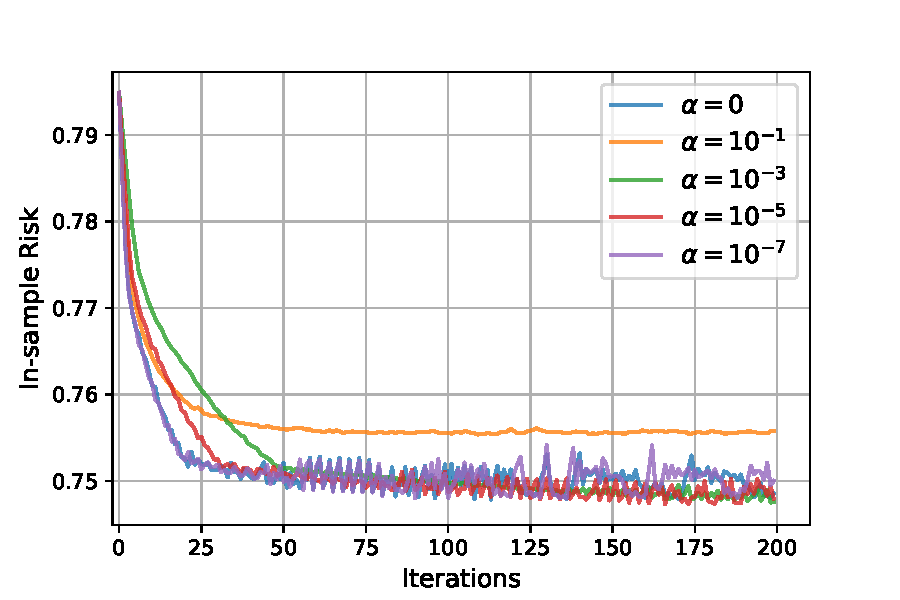
\includegraphics[width=0.46\textwidth]{Images/convergence_toy.pdf}
%     \caption{Caption}
%     \label{fig:toy_example_cvgence}
% \end{figure}
\begin{figure*}[!ht]
\begin{center}

\textbf{Adversarial Training, CIFAR-10 dataset results}
 \begin{small}
\begin{tabular}{c|c|ccc} 
\textbf{ Models} & \textbf{Acc. }&\textbf{$\textrm{APGD}_\textrm{CE}$}& \textbf{$\textrm{APGD}_\textrm{DLR}$} & \textbf{Rob. Acc.} \\ \hline
 1 & $81.9\%$ &	$47.6\%$ & $47.7\%$ & $45.6\%$ \\ 
 2 & $81.9\%$ & $49.0\%$ & ${49.6\%}$ & ${47.0\%}$\\ 
  3 & ${81.7\%}$& ${49.0\%}$ & $49.3\%$ & ${46.9\%}$\\
    4 & $\bm{82.6\%}$& $\bm{49.7\%}$ & $\bm{49.8}\%$ & $\bm{47.2\%}$\\

\end{tabular}
\end{small}\\
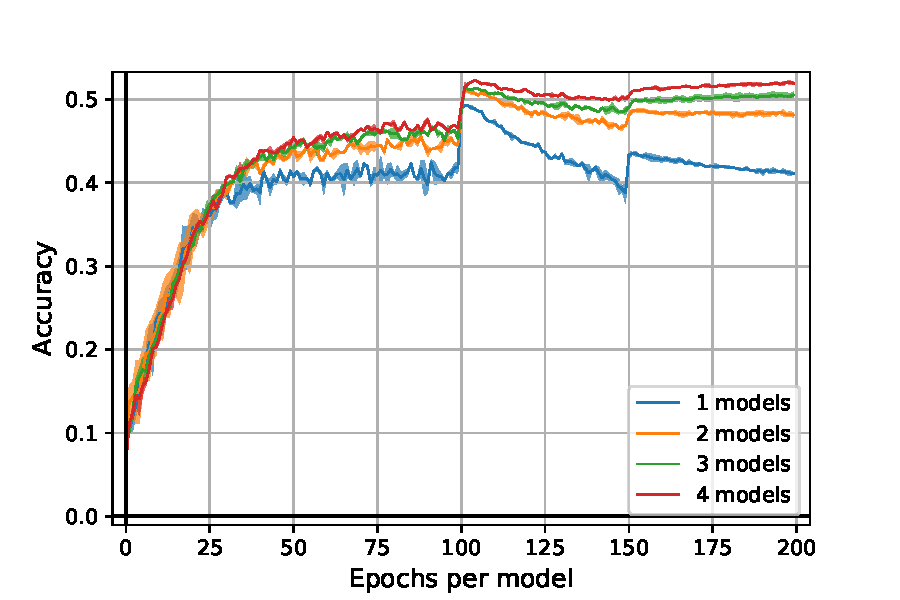
\includegraphics[width=0.35\textwidth]{Images/robust_acc_finalrun_ResNet18_1024_200_0.001.pdf}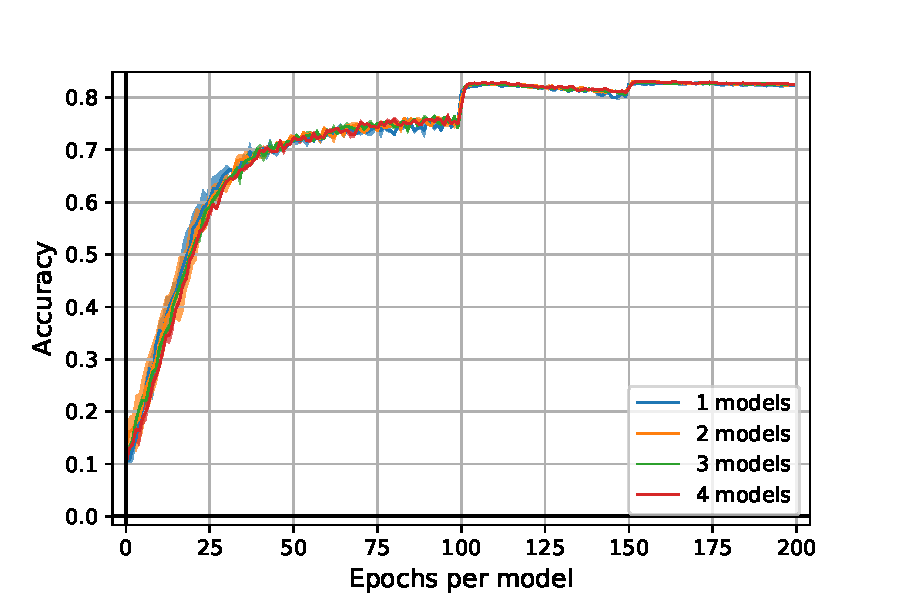
\includegraphics[width=0.35\textwidth]{Images/standard_acc_finalrun_ResNet18_1024_200_0.001.pdf} 
  

\textbf{TRADES, CIFAR-10 dataset results}

 \begin{small}
\begin{tabular}{c|c|ccc} 
\textbf{ Models} & \textbf{Acc. }&\textbf{$\textrm{APGD}_\textrm{CE}$}& \textbf{$\textrm{APGD}_\textrm{DLR}$} & \textbf{Rob. Acc.} \\ \hline
 1 &  $79.6\%$ &$50.9\%$& $48.9\%$ &$48.3\%$ \\ 
 2 & $80.3\%$& $52.3\%$ &$51.2\%$ &$50.2\%$\\ 
  3 & $80.7\%$& $52.8\%$ &$51.7\%$ &$50.7\%$\\
    4 & \bm{$80.9\%$} & \bm{$53.0\%$}& \bm{$51.8\%$}& \bm{$50.8\%$}\\

\end{tabular}
\end{small}

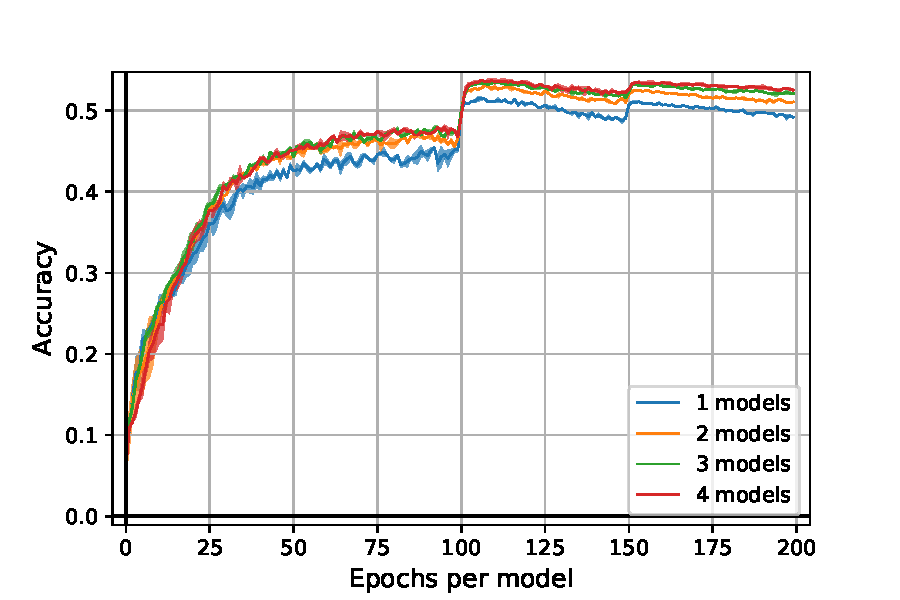
\includegraphics[width=0.35\textwidth]{Images/robust_acc_CIFAR10_final_cam_ready_bisss_ResNet18_1024_200_0.001.pdf}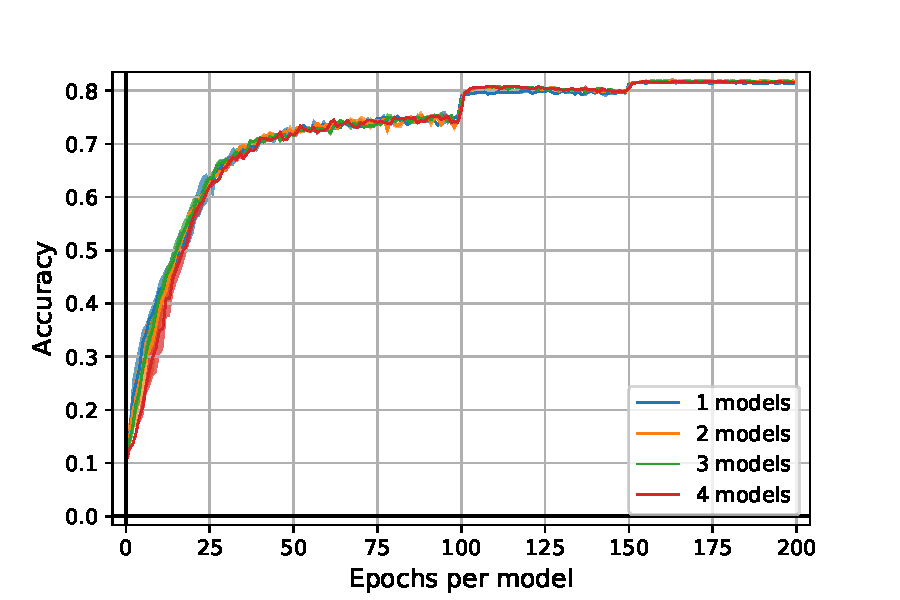
\includegraphics[width=0.35\textwidth]{Images/standard_acc_CIFAR10_final_cam_ready_bisss_ResNet18_1024_200_0.001.pdf} 
  

\textbf{Adversarial Training, CIFAR-100 dataset results}
 \begin{small}
\begin{tabular}{c|c|ccc} 
\textbf{ Models} & \textbf{Acc. }&\textbf{$\textrm{APGD}_\textrm{CE}$}& \textbf{$\textrm{APGD}_\textrm{DLR}$} & \textbf{Rob. Acc.} \\ \hline
 1 & $55.2\%$& $24.1\%$& $23.8\%$ & $22.5\%$\\ 
 2 & $55.2\%$ & $25.3\%$ &$26.1\%$ &$23.6\%$\\ 
  3 & \bm{$55.4\%$} & $25.7\%$ &$26.8\%$ &$24.2\%$\\
    4 & $55.3\%$ & \bm{$26.0\%$} & \bm{$27.5\%$}& \bm{$24.5\%$}\\

\end{tabular}
\end{small}
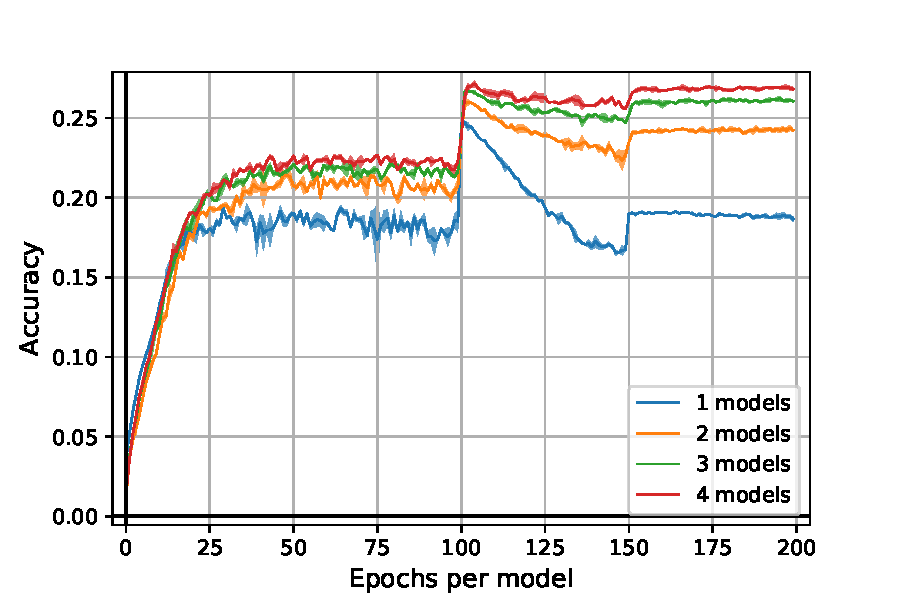
\includegraphics[width=0.35\textwidth]{Images/robust_acc_CIFAR100_finalrun_ResNet18_1024_200_0.001.pdf}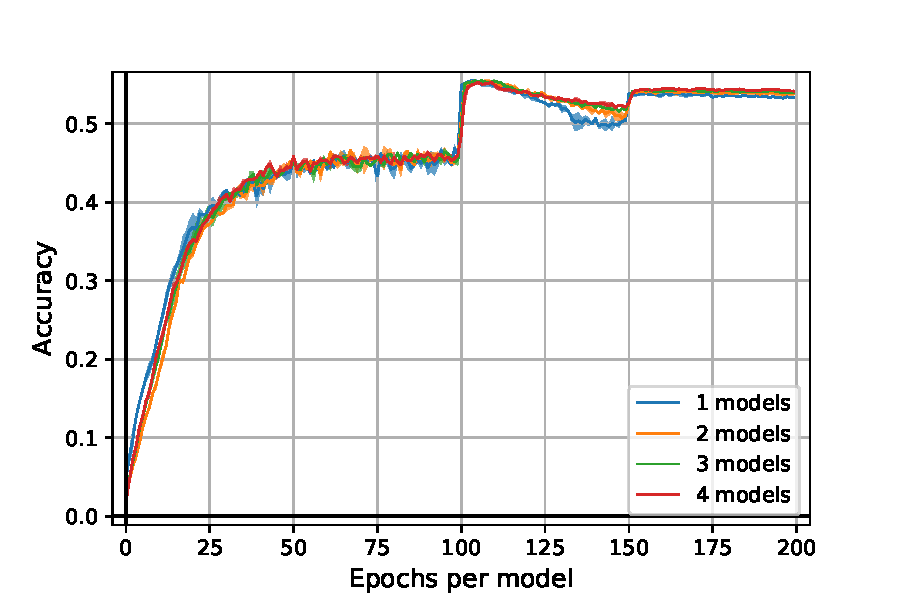
\includegraphics[width=0.35\textwidth]{Images/standard_acc_CIFAR100_finalrun_ResNet18_1024_200_0.001.pdf} 


 \caption{Upper plots: Adversarial Training, CIFAR-10 dataset results. Middle plots:  TRADES, CIFAR-10 dataset results. Bottom plots: CIFAR-100 dataset results. {On left}: Comparison of our algorithm with a standard adversarial training (one model). We reported the results for the model with the best robust accuracy obtained over two independent runs because adversarial training might be unstable. Standard and Robust accuracy (respectively in the middle and on right) on CIFAR-10 test images in function of the number of epochs per classifier with $1$ to $3$ ResNet18 models. The performed attack is PGD with $20$ iterations and $\varepsilon=8/255$.}
\label{fig:results_cifar}

\end{center}
\end{figure*}

To evaluate the convergence of our algorithms, we compute the adversarial risk of our mixture for each iteration of both the oracle and regularized algorithms. Figure~\ref{fig:toy_example} illustrates the convergence of the algorithms w.r.t the regularization parameter. We observe that the risk for both algorithms converge. Moreover, they converge towards the oracle minimizer when the regularization parameter $\alpha$ goes to $0$.

Finally, to demonstrate the improvement randomized techniques offer against deterministic defenses, we plot in Figure~\ref{fig:toy_example} (right) the minimum adversarial risk for both randomized and deterministic classifiers w.r.t. $\varepsilon$. The adversarial risk is strictly better for randomized classifier whenever the adversarial budget $\varepsilon$ is bigger than $2$. This illustration validates our analysis of Theorem~\ref{thm:duality-rand}, and motivates a in depth study of a more challenging framework, namely image classification with neural networks.

% \begin{figure}[ht]
%     \centering
%     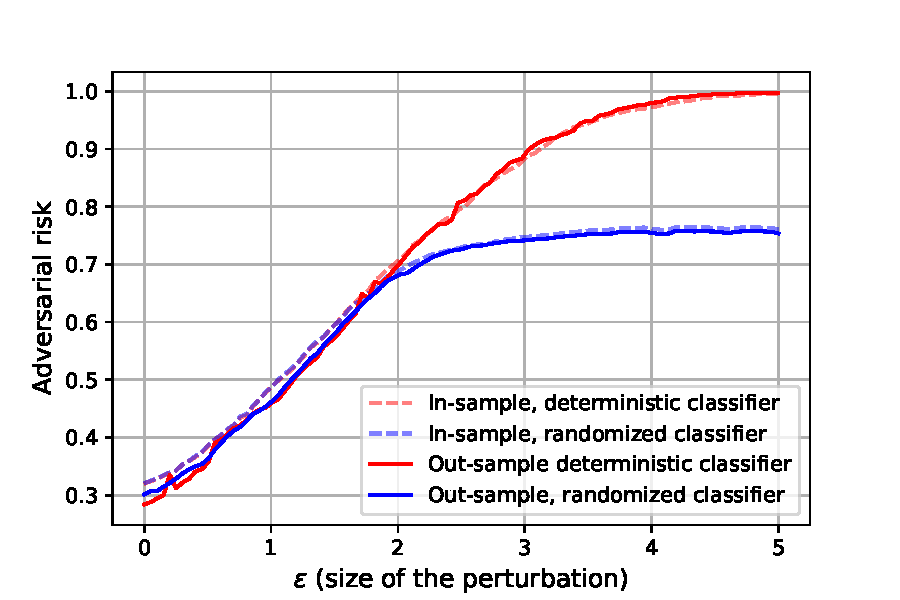
\includegraphics[width=0.46\textwidth]{Images/risk_toy.pdf}
%     \caption{Caption}
%     \label{fig:toy_example_risk}
% \end{figure}

\subsection{CIFAR Datasets}

% \begin{figure*}[!ht]
% \begin{center}

% \vskip 0.15in
%  \begin{minipage}[ht!]{0.39\textwidth}
%  \begin{scriptsize}
% \begin{tabular}{c|c|ccc} 
% \textbf{ Models} & \textbf{Acc. }&\textbf{$\textrm{APGD}_\textrm{CE}$}& \textbf{$\textrm{APGD}_\textrm{DLR}$} & \textbf{Rob. Acc.} \\ \hline
%  1 & $81.9\%$ &	$47.6\%$ & $47.7\%$ & $45.6\%$ \\ 
%  2 & $81.9\%$ & $49.0\%$ & ${49.6\%}$ & ${47.0\%}$\\ 
%   3 & ${81.7\%}$& ${49.0\%}$ & $49.3\%$ & ${46.9\%}$\\
%     4 & $\bm{82.6\%}$& $\bm{49.7\%}$ & $\bm{49.8}\%$ & $\bm{47.2\%}$\\

% \end{tabular}
% \end{scriptsize}
%   \end{minipage}\begin{minipage}[!ht]{0.61\textwidth}
% 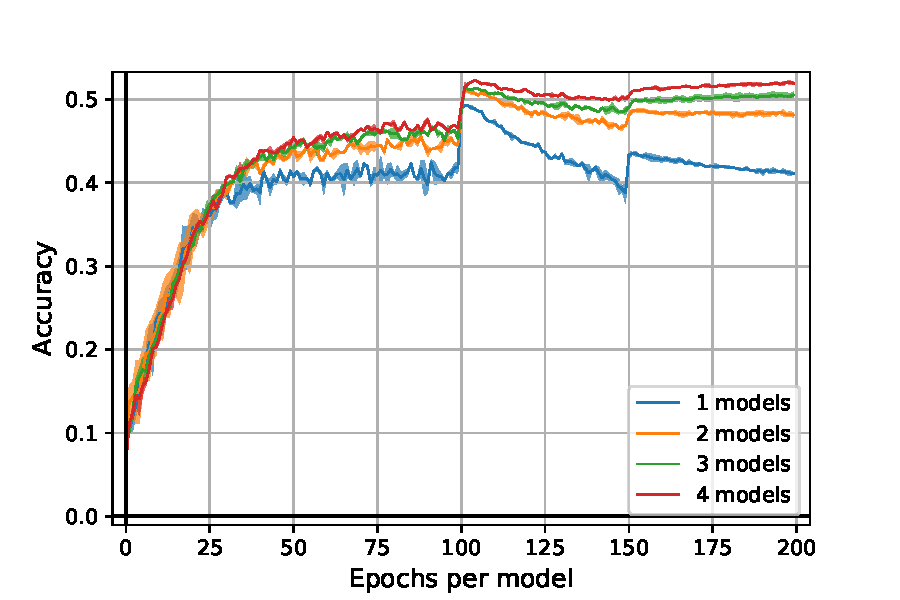
\includegraphics[width=0.49\textwidth]{Images/robust_acc_finalrun_ResNet18_1024_200_0.001.pdf}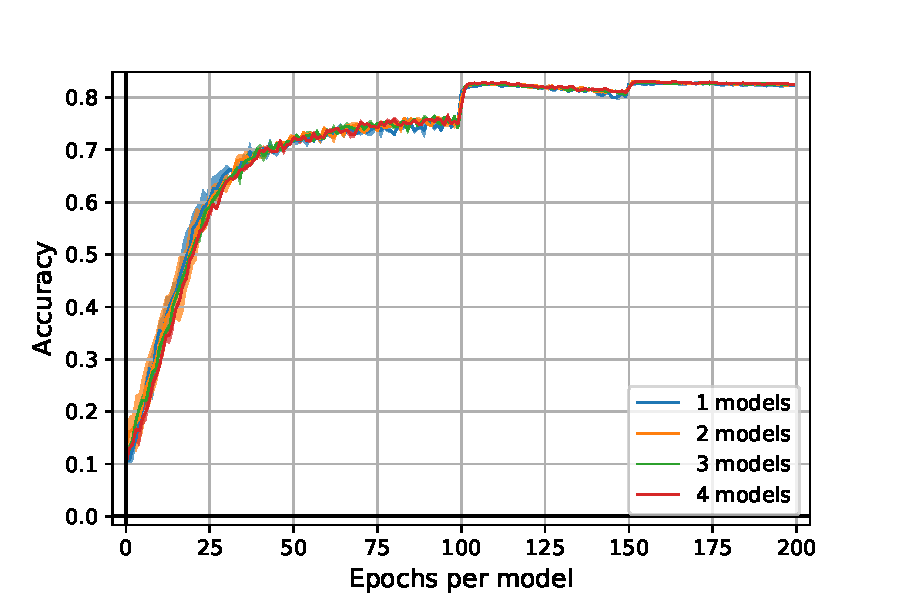
\includegraphics[width=0.49\textwidth]{Images/standard_acc_finalrun_ResNet18_1024_200_0.001.pdf} 
%   \end{minipage}
  
% Adversarial Training, CIFAR-10 dataset results

% \vskip 0.15in
%  \begin{minipage}[ht!]{0.39\textwidth}
%  \begin{scriptsize}
% \begin{tabular}{c|c|ccc} 
% \textbf{ Models} & \textbf{Acc. }&\textbf{$\textrm{APGD}_\textrm{CE}$}& \textbf{$\textrm{APGD}_\textrm{DLR}$} & \textbf{Rob. Acc.} \\ \hline
%  1 &  $79.6\%$ &$50.9\%$& $48.9\%$ &$48.3\%$ \\ 
%  2 & $80.3\%$& $52.3\%$ &$51.2\%$ &$50.2\%$\\ 
%   3 & $80.7\%$& $52.8\%$ &$51.7\%$ &$50.7\%$\\
%     4 & \bm{$80.9\%$} & \bm{$53.0\%$}& \bm{$51.8\%$}& \bm{$50.8\%$}\\

% \end{tabular}
% \end{scriptsize}
%   \end{minipage}\begin{minipage}[!ht]{0.61\textwidth}
% 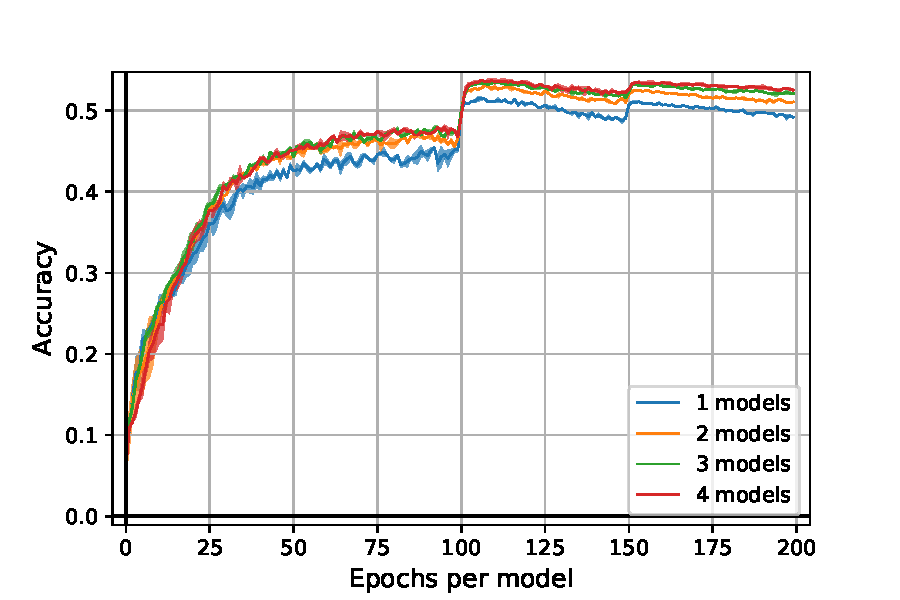
\includegraphics[width=0.49\textwidth]{Images/robust_acc_CIFAR10_final_cam_ready_bisss_ResNet18_1024_200_0.001.pdf}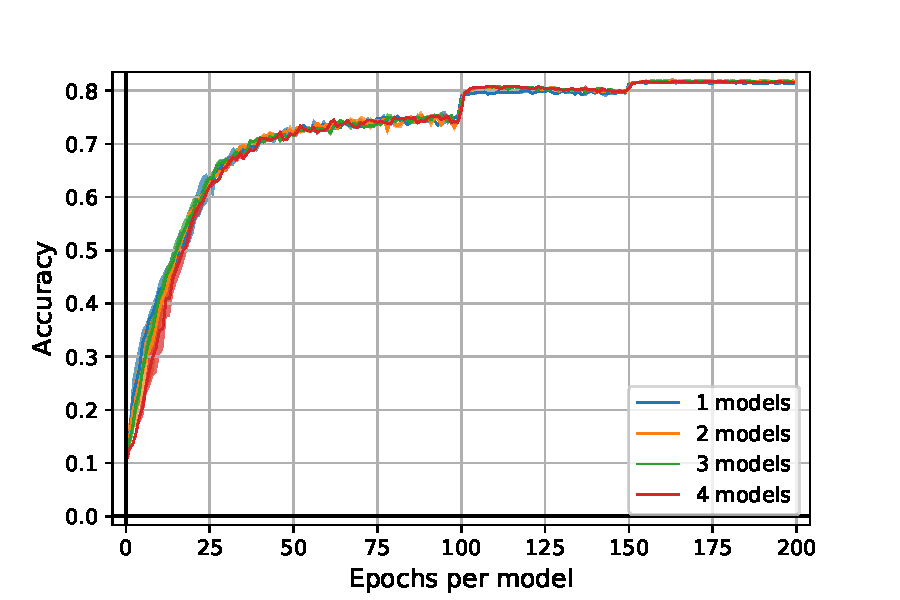
\includegraphics[width=0.49\textwidth]{Images/standard_acc_CIFAR10_final_cam_ready_bisss_ResNet18_1024_200_0.001.pdf} 
%   \end{minipage}
  
% TRADES, CIFAR-10 dataset results
% \vskip 0.15in
%  \begin{minipage}[ht!]{0.39\textwidth}
%  \begin{scriptsize}
% \begin{tabular}{c|c|ccc} 
% \textbf{ Models} & \textbf{Acc. }&\textbf{$\textrm{APGD}_\textrm{CE}$}& \textbf{$\textrm{APGD}_\textrm{DLR}$} & \textbf{Rob. Acc.} \\ \hline
%  1 & $55.2\%$& $24.1\%$& $23.8\%$ & $22.5\%$\\ 
%  2 & $55.2\%$ & $25.3\%$ &$26.1\%$ &$23.6\%$\\ 
%   3 & \bm{$55.4\%$} & $25.7\%$ &$26.8\%$ &$24.2\%$\\
%     4 & $55.3\%$ & \bm{$26.0\%$} & \bm{$27.5\%$}& \bm{$24.5\%$}\\

% \end{tabular}
% \end{scriptsize}
%   \end{minipage}\begin{minipage}[!ht]{0.61\textwidth}
% 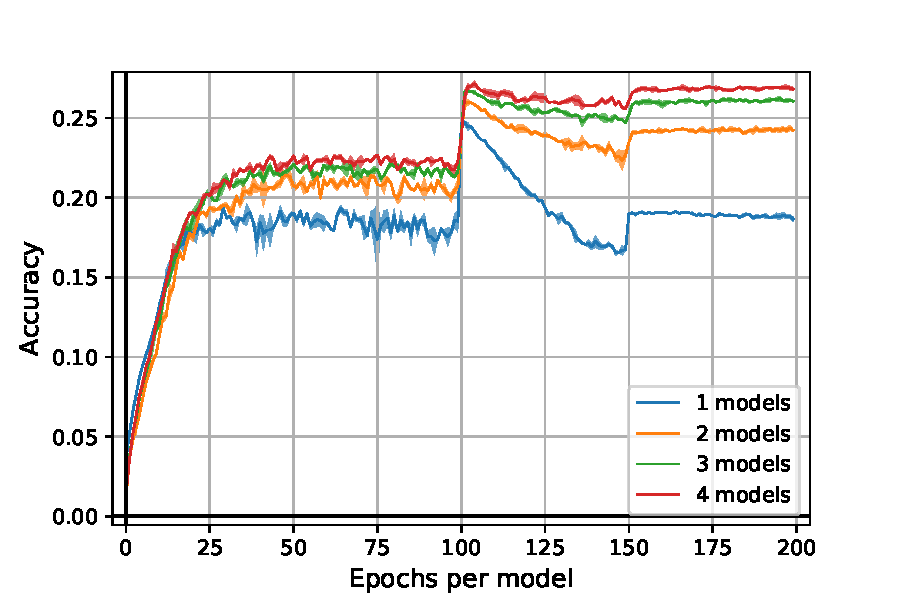
\includegraphics[width=0.49\textwidth]{Images/robust_acc_CIFAR100_finalrun_ResNet18_1024_200_0.001.pdf}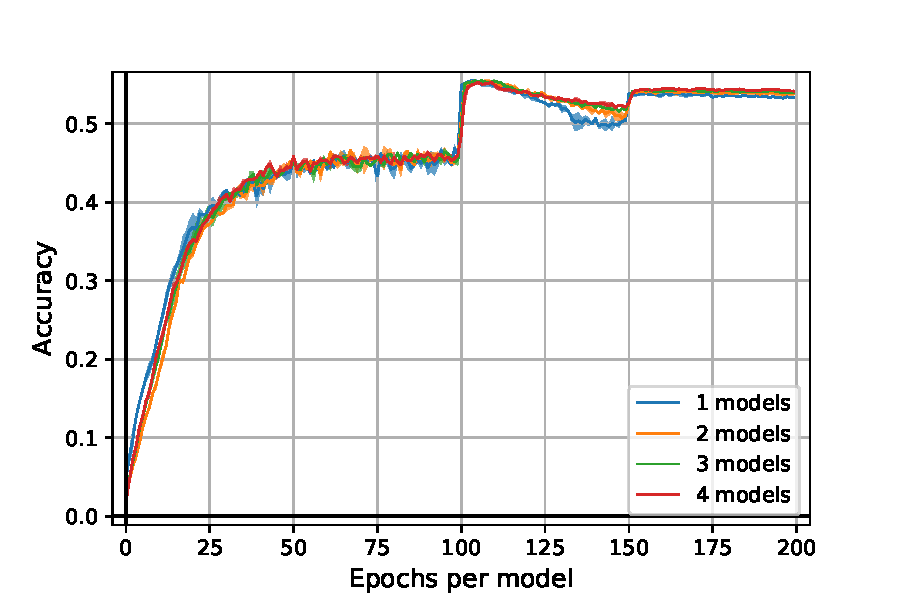
\includegraphics[width=0.49\textwidth]{Images/standard_acc_CIFAR100_finalrun_ResNet18_1024_200_0.001.pdf} 
%   \end{minipage}
%   Adversarial Training, CIFAR-100 dataset results

%  \caption{Upper plots: Adversarial Training, CIFAR-10 dataset results. Middle plots:  TRADES, CIFAR-10 dataset results. Bottom plots: CIFAR-100 dataset results. {On left}: Comparison of our algorithm with a standard adversarial training (one model). We reported the results for the model with the best robust accuracy obtained over two independent runs because adversarial training might be unstable. Standard and Robust accuracy (respectively in the middle and on right) on CIFAR-10 test images in function of the number of epochs per classifier with $1$ to $3$ ResNet18 models. The performed attack is PGD with $20$ iterations and $\varepsilon=8/255$.}
% \label{fig:results_cifar}

% \end{center}
% \end{figure*}

% Adversarial examples are known to be easily transferrable from one model to another~\cite{tramer2017space}. To counter this and support our theoretical claims, we propose an heuristic algorithm (see Algorithm~\ref{algo:heuristic}) to train a robust mixture of $L$ classifiers. We alternatively train these classifiers with adversarial examples against the current mixture and update the probabilities of the mixture according to the algorithms we proposed in Section~\ref{sec:proposed-algo}. More details on the heuristic algorithm are available in Appendix~\ref{sec:additional-xp}. 
% \begin{algorithm}[h!]
% \small
% \SetAlgoLined
% $L$: number of models, $T$: number of iterations,\\
% $T_\theta$: number of updates for the models $\bm{\theta}$,\\
% $T_\lambda$: number of updates for the mixture $\bm{\lambda}$,\\ $\bm{\lambda}_0=(\lambda_0^1,\dots\lambda_0^L),~\bm{\theta}_0=(\theta_0^1,\dots\theta_0^L)$\\
%  \For{$t=1,\dots,T$}{
%  Let $B_t$ be a batch of data.\\
% \eIf{$t \mod (T_\theta L+1)\neq 0$}{
% $k$ sampled uniformly in $\{1,\dots,L\}$\\
% $\Tilde{B}_t\leftarrow$ Attack of images in $B_t$ for the  model $(\bm{\lambda}_t,\bm{\theta}_t)$\\
% $\theta^t_k\leftarrow$ Update $\theta^{t-1}_k$ with $\Tilde{B}_t$ for fixed $\bm{\lambda}_t$ with a SGD step}{
% $\bm{\lambda}_t\leftarrow$Update $\bm{\lambda}_{t-1}$ on $B_t$ for fixed $\bm{\theta}_t$
% with oracle or regularized algorithm with $T_\lambda$ iterations.
% }
%   }
%  \caption{Adversarial Training for Mixtures}
 
%  \label{algo:heuristic}
% \end{algorithm}

\paragraph{Experimental Setup.} We now implement our heuristic algorithm (Alg.~\ref{algo:heuristic}) on CIFAR-10 and CIFAR-100 datasets for both Adversarial Traning~\citep{madry2017towards} and TRADES~\citep{zhang2019theoretically} loss. To evaluate the performance of Algorithm~\ref{algo:heuristic}, we trained from $1$ to $4$ ResNet18~\citep{He_2016_CVPR} models on $200$ epochs per model\footnote{$L\times200$ epochs in total, where $L$ is the number of models.}. We study the robustness with regards to $\ell_\infty$ norm and fixed adversarial budget $\varepsilon=8/255$. The attack we used in the inner maximization of the training is an adapted (adaptative) version of PGD for mixtures of classifiers with $10$ steps. Note that for one single model, Algorithm~\ref{algo:heuristic} exactly corresponds to adversarial training~\citep{madry2017towards} or TRADES. For each of our setups, we made two independent runs and select the  best one. The training time of our algorithm is around four times longer than a standard Adversarial Training (with PGD 10 iter.) with two models, eight times with three models and twelve times with four models. We trained our models with a batch of size  $1024$ on $8$ Nvidia V100 GPUs. 

\paragraph{Optimizer.} For each of our models, The optimizer we used in all our implementations is SGD with learning rate set to $0.4$ at epoch $0$ and is divided by $10$ at half training then by $10$ at the three quarters of training. The momentum is set to $0.9$ and the weight decay to $5\times10^{-4}$. The batch size is set to $1024$. 
\paragraph{Adaptation of Attacks.} Since our classifier is randomized, we need to adapt the attack accordingly. To do so we used the expected loss:
\begin{align*}
\Tilde{\loss}\left((\bm{\lambda},\bm{\theta}),(x,y)\right) = \sum_{k=1}^L \lambda_k \loss(\theta_k,(x,y))
\end{align*}
to compute the gradient in the attacks, regardless the loss (DLR or cross-entropy). For the inner maximization at training time, we used a PGD attack on the cross-entropy loss with $\varepsilon=0.03$. For the final evaluation, we used the untargeted $DLR$ attack with default parameters.
\paragraph{Regularization in Practice.} The entropic regularization in higher dimensional setting need to be adapted to be more likely to find adversaries. To do so, we computed PGD attacks with only $3$ iterations with $5$ different restarts instead of sampling uniformly $5$ points  in the $\ell_\infty$-ball. In our experiments in the main paper, we use a regularization parameter $\alpha=0.001$. The learning rate for the minimization on $\bm{\lambda}$ is always fixed to $0.001$. 
\paragraph{Alternate Minimization Parameters.} Algorithm~\ref{algo:heuristic} implies an alternate minimization algorithm. We set the number of updates of $\bm{\theta}$ to $T_\theta = 50$ and, the update of $\bm{\lambda}$ to $T_\lambda = 25$. 

\subsection{Effect of the Regularization}
In this subsection, we experimentally investigate the effect of the regularization. In Figure~\ref{fig:xp-regularization}, we notice, that the regularization has the effect of stabilizing, reducing the variance and improving the level of the robust accuracy for adversarial training for mixtures (Algorithm~\ref{algo:heuristic}). The standard accuracy curves are very similar in both cases.



\paragraph{Evaluation Protocol.} At each epoch, we evaluate the current mixture on test data against PGD attack  with $20$ iterations. To select our model and avoid overfitting~\citep{rice2020overfitting}, we kept the most robust against this PGD attack.
To make a final evaluation of our mixture of models, we used an adapted version of $\textrm{AutoPGD}$ untargeted attacks~\citep{croce2020reliable} for randomized classifiers with both Cross-Entropy (CE) and Difference of Logits Ratio (DLR) loss. For both attacks, we made $100$ iterations and $5$ restarts.

\paragraph{Results.} The results are presented in Figure~\ref{fig:results_cifar}. We remark our algorithm outperforms a standard adversarial training in all the cases by more $1\%$ on CIFAR-10 and CIFAR-100, without additional loss of standard accuracy as it is attested by the left figures. On TRADES, the gain is even more important by more than $2\%$ in robust accuracy. Moreover, it seems our algorithm, by adding more and more models, reduces the overfitting of adversarial training. It also appears that robustness increases as the number of models increases. So far, experiments are computationally very costful and it is difficult to raise precise conclusions. Further, hyperparameter tuning ~\citep{gowal2020uncovering} such as architecture, unlabeled data~\citep{carmon2019unlabeled} or activation function may still increase the results.





% \begin{figure*}[!ht]
% \begin{center}


% \label{table:results}
% \vskip 0.15in
%  \begin{minipage}[!ht]{0.39\textwidth}
%  \begin{scriptsize}
% \begin{tabular}{c|c|ccc} 
% \textbf{ Models} & \textbf{Acc. }&\textbf{$\textrm{APGD}_\textrm{CE}$}& \textbf{$\textrm{APGD}_\textrm{DLR}$} & \textbf{Rob. Acc.} \\ \hline
%  1 & $81.9\%$ &	$47.6\%$ & $47.7\%$ & $45.6\%$ \\ 
%  2 & $81.9\%$ & $49.0\%$ & ${49.6\%}$ & ${47.0\%}$\\ 
%   3 & ${81.7\%}$& ${49.0\%}$ & $49.3\%$ & ${46.9\%}$\\
%     4 & $\bm{82.6\%}$& $\bm{49.7\%}$ & $\bm{49.8}\%$ & $\bm{47.2\%}$\\

% \end{tabular}
% \end{scriptsize}
%   \end{minipage}\begin{minipage}[!ht]{0.61\textwidth}
% 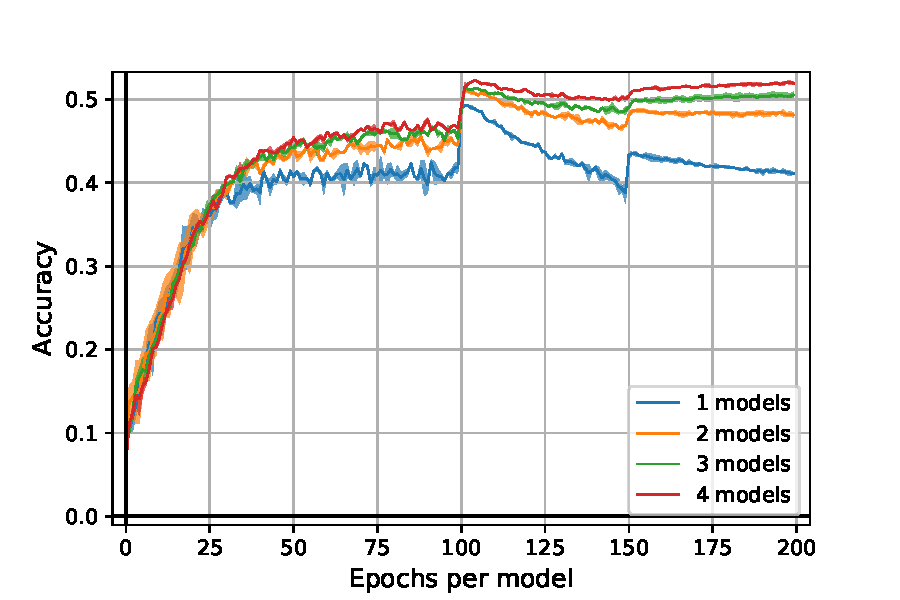
\includegraphics[width=0.49\textwidth]{Images/robust_acc_finalrun_ResNet18_1024_200_0.001.pdf}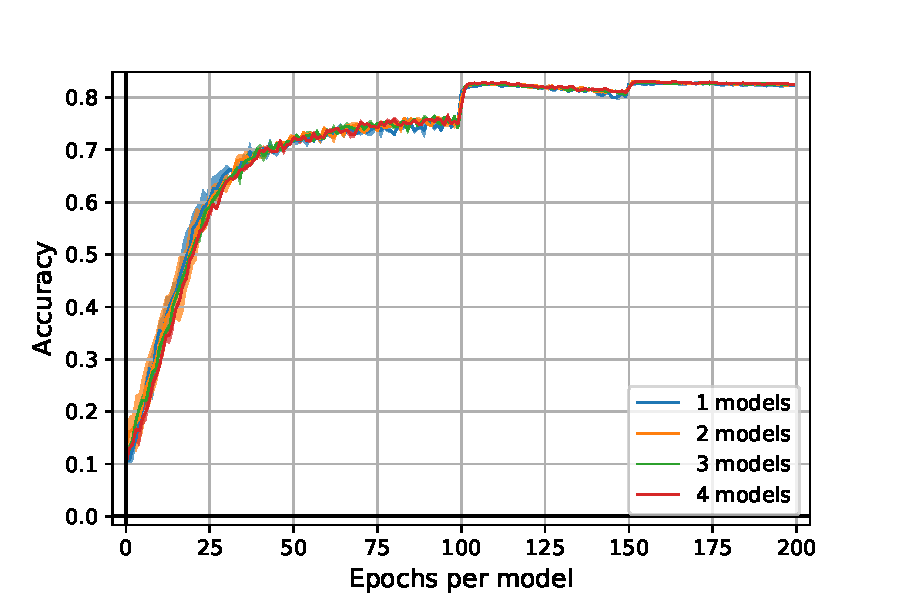
\includegraphics[width=0.49\textwidth]{Images/standard_acc_finalrun_ResNet18_1024_200_0.001.pdf} 
%   \end{minipage}
  
% \caption{On left: Comparison of our algorithm with a standard adversarial training (one model). We reported the results for the model with the best robust accuracy obtained over two independent runs because adversarial training might be unstable. Standard and Robust accuracy ( respectively in the center and on left) on CIFAR-10 test images in function of the number of epochs per classifier with $1$ to $3$ ResNet18 models. The performed attack is PGD with $20$ iterations and $\varepsilon=8/255$.}
% \label{fig:results_cifar}
% \end{center}
% \end{figure*}











% \begin{figure}[!ht]
% 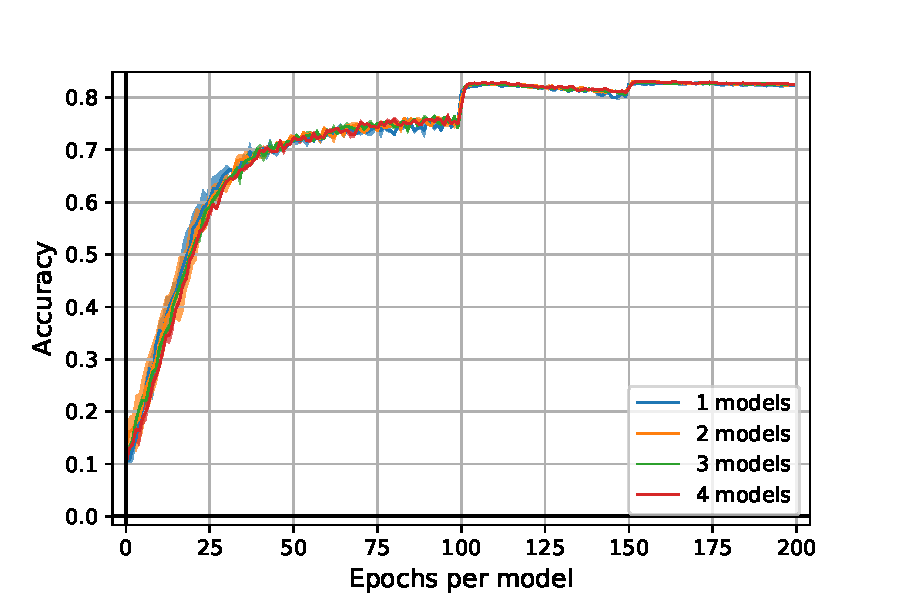
\includegraphics[width=0.46\textwidth]{Images/standard_acc_finalrun_ResNet18_1024_200_0.001.pdf}    \caption{Standard accuracy on CIFAR-10 test images in function of the number of epochs per classifier with $1$ to $3$ ResNet18 models.}
%     \label{fig:plot_standard_acc}
% \end{figure}

% \begin{figure}[!ht]
% 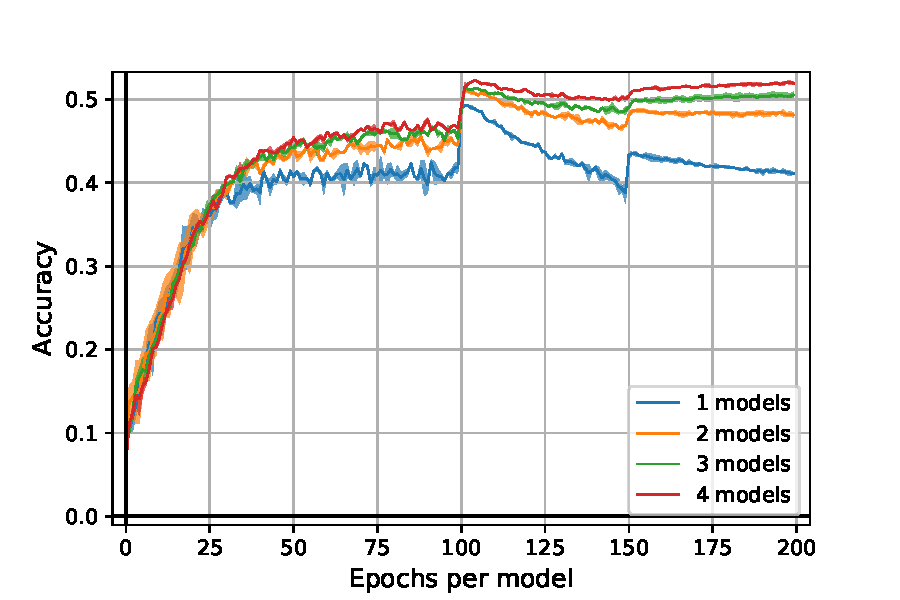
\includegraphics[width=0.46\textwidth]{Images/robust_acc_finalrun_ResNet18_1024_200_0.001.pdf}    \caption{Robust accuracy on CIFAR-10 test images in function of the number of epochs per classifier with $1$ to $3$ ResNet18 models. The attack performed is PGD with $20$ iterations and $\varepsilon=8/255$.}
%     \label{fig:plot_robust_acc}
% \end{figure}



% mettre ca au propre mais les resultats sont la!!

% setup: ResNet18 ou WRN28x10

% Details in supmat: loss +lr + format of training etc

% In supmat: 
% \begin{enumerate}
%     \item details HP (attack + training)
%     \item details runtime
%     \item additional results (with other attacks maybe + other archis...)
    
    
% \end{enumerate}
% Epochs 100

\section{Conclusion}
We presented several settings for online attacks on contextual bandits.
We showed that an attacker can force any contextual bandit algorithm to almost always pull an arbitrary target arm $a^{\dagger}$ with only sublinear modifications of the rewards. When the attacker can only modify the contexts, we prove that \linucb can still be attacked and made to almost always pull an arm in $A^{\dagger}$ by adding sublinear perturbations to the contexts. 
When the attacker can only attack a single context, we derive a feasibility condition for the attacks and we introduce a method to compute some attacks of small instantaneous cost for \linucb, \epsgreedy and \lints.
To the best of our knowledge, this paper is the first to describe effective attacks on the contexts of contextual bandit algorithms. Our numerical experiments, conducted on both synthetic and real-world data, validate our results and show that the attacks on all contexts are actually effective on several algorithms and with more permissible settings. 





\begin{subappendices}
% !TEX root = main.tex

\section{Appendix: Proofs}
In this appendix, we present the proofs of different theoretical results presented in the paper.
\subsection{Proof of Proposition \ref{prop:reward_attack}}\label{app:proof_prop_rewd_attack}

\begin{prop*}
	For any $\delta\in(0, 1/K]$, when using Contextual ACE algorithm (Alg. ~\ref{alg:attacker_rewards}) with perturbed rewards $\tilde{r}^{1}$, with probability at least $1-K\delta$, algorithm $\mathfrak{A}$ pulls \changelm{an arm in $A^{\dagger}$} for $T - o(T)$ time steps and the total cost of attacks is $o(T)$.
\end{prop*}

\begin{proof}
	Let us consider the contextual bandit problem $\mathcal{A}_{1}$, with $K$ arms with contexts $x\in \mathcal{D}$ such that every arm in \changelm{$a^\dagger\in A^\dagger$ has mean reward $\langle \theta_{a^{\dagger}}, x\rangle$} and all other arms has mean $0$. Then the regret of algorithm $\mathfrak{A}$ for this bandit problem is upper-bounded with probability at least $1 - \delta$ by a function $f_{\mathfrak{A}}(T)$ such that $f_{\mathfrak{A}}(T) = o(T)$. In addition, the reward process fed to Alg. $\mathfrak{A}$ by the attacker is a stationary reward process with $\sigma^{2}$-subgaussian noise. Therefore, the number of times algorithm $\mathfrak{A}$ pulls an arm \changelm{not in $A^{\dagger}$ is upper-bounded by \changee{$f_{\mathfrak{A}}(T)/\min_{x\in \mathcal{D}} \Delta(x)$ where for every context $x\in\mathcal{D}$, let $a
^{\dagger}_{\star}(x) := \arg\max_{a\in A^{\dagger}} \langle x, \theta_{a}\rangle$ and $\Delta(x) = \langle x, \theta_{a^{\dagger}_{\star}(x)}\rangle - \max_{a\in A^{\dagger}, a\neq a_{\star}^{\dagger}(x)} \langle x, \theta_{a}\rangle$}}. 

\changelm{In addition, the total cost of the attack is upper-bounded by $\max_{a\in \llbracket 1, K\rrbracket} \max_{x\in \mathcal{D}} |\langle x, \theta_{a}\rangle| (T - N_{A^{\dagger}}(T))$ where $N_{A^{\dagger}}(T)$ is the number of times an arm  in $A^{\dagger}$ has been pulled up to time $T$. Thanks to the previous argument, $T - N_{A^{\dagger}}(T) \leq  f_{\mathfrak{A}}(T)/\min_{x\in \mathcal{D}}\Delta(x)$.}
\end{proof}
% \subsection{Proof of Proposition \ref{prop:cost_attack_all_ctx}:}
% \begin{proof}
% The bound of the number of times the arm $a^*$ is the same as for proposition \ref{prop:reward_attack}.
% As the attacker only attacks when the arm $a^{\star}$ is not pulled and the contexts are bounded by 1, the total cost of each attack is upper bounded by $\delta$, hence the bound on the total cost of the attacks.

% \end{proof}

\subsection{Proof of Proposition \ref{prop:cost_attack_all_ctx}}\label{app:proof_attack_all_ctx}

\begin{prop*}
Using the attack described in Alg.~\ref{alg:context_attack_protocol}, for any $\delta\in (0, 1/K]$, with probability at least $1 - K\delta$, the number of times \linucb does not pull \changelm{an arm in $A^{\dagger}$} is at most:
\begin{align*}
    \sum_{j\changelm{\notin A^{\dagger}}} N_{j}(T) \leq 32K^{2}\left( \frac{\lambda}{\alpha^{2}} + \sigma^{2}d\log\left(\frac{\lambda d + TL^2\alpha^{2}}{d\lambda\delta}\right) \right)^{3}
\end{align*}
with $N_{j}(T)$ the number of times arm $j$ has been pulled after $T$ steps, $|| \theta_{a}|| \leq S$ for all arms $a$, $\lambda$ the regularization parameter of \linucb and for all $x\in \mathcal{D}$, $||x||_{2}\leq L$. The total cost for the attacker is bounded by:
\begin{align*}
    \sum_{t=1}^{T} c_{t} \leq \frac{64K^{2}}{\nu}\left( \frac{\lambda}{\alpha^{2}} + \sigma^{2}d\log\left(\frac{\lambda d + TL^2\alpha^{2}}{d\lambda\delta}\right) \right)^{3}
\end{align*}
\end{prop*}

\begin{proof}
Let $a_{t}$ be the arm pulled by \linucb at time $t$. For each arms $a$, let $\tilde{\theta}_a(t)$ be the result of the linear regression with the attacked context and $\hat{\theta}_{a}(t, \lambda/\alpha^{2})$ the one with the unattacked context and a regularization of $\frac{\lambda}{\alpha^{2}}$. At any time step $t$, we can write, for all $a\changebrtwo{\not\in A^\dagger}$:

\begin{align*}
\tilde{\theta}_a(t) &=  \left(\lambda I_d + \sum_{l=0, a_{l} = a}^{t} \alpha^{2} x_l x_l^{\intercal}\right)^{-1} \sum_{k=0, a_{k} = a}^{t} r_k \alpha x_{k} \\
&= \frac{1}{\alpha} \left(\frac{\lambda}{\alpha^2} I_d + \sum_{k=0, a_{k} = a}^t x_k x_k^{\intercal}\right)^{-1} \sum_{k=0, a_{k} = a}^t r_k x_k \\
&= \frac{\hat{\theta}_{a}(t,\lambda/\alpha^{2})}{\alpha}
\end{align*}
\changelm{We also note that, since the contexts are not modified for arms in  $a^\dagger\in A^\dagger$: $\tilde{\theta}_{a^\dagger}(t)=\hat{\theta}_{a^\dagger}(t,\lambda)$. In addition, for any context $x$ and arm $a\notin A^\dagger$, the exploration term used by \linucb becomes:}
\begin{align}
    ||x||_{\tilde{V}_{a,t}^{-1}}&= \frac{1}{\alpha} ||x||_{\hat{V}_{a,t}^{-1}}
\end{align}
where $\tilde{V}_{a,t} = \lambda I_d + \sum_{l=0, a_{l} = a}^{t} \alpha^{2} x_l x_l^{\intercal}$ and $\hat{V}_{a,t}^{-1} =\lambda/ \alpha^2 I_d + \sum_{k=0, a_{k} = a}^t x_k x_k^{\intercal}$. For a time $t$, if presented with context $x_{t}$ \linucb pulls arm \changelm{$a_{t} \notin A^{\dagger}$,} we have:
\begin{align*}
\alpha\left(\left\langle \hat{\theta}_{a^\dagger}(t), x_{t} \right\rangle +\beta_{a^\dagger}(t)||x_t||_{V_{a^\dagger,t}^{-1}}\right)\leq \left\langle \hat{\theta}_{a_{t}}(t, \lambda/\alpha^{2}), x_{t} \right\rangle +  \beta_{a_{t}}(t)||x_{t}||_{\hat{V}_{a_{t},t}^{-1}} 
\end{align*}

As \changelm{$\alpha = \frac2\nu\geq\min_{a^\dagger\in A^\dagger}\frac{2}{\left\langle \theta_{a^\dagger}, x_{t} \right\rangle}$}, we deduce that on the event that the confidence sets (Theorem $2$ in \cite{abbasi2011improved}) hold for arm $a^{\star}$: 
\begin{align*}
    2&\leq\left\langle \hat{\theta}_{a_{t}}(t, \lambda/\alpha^{2}), x_{t} \right\rangle +  \beta_{a_{t}}(t)||x_{t}||_{\hat{V}_{a_{t},t}^{-1}}\leq \langle\theta_{a_{t}}, x_{t}\rangle+2\beta_{a_{t}}(t)||x_{t}||_{\hat{V}_{a_{t},t}^{-1}}
\end{align*}
Thus, $1 \leq 2 - \langle\theta_{a_{t}}, x_{t}\rangle \leq 2\beta_{a_{t}}(t)||x_{t}||_{\hat{V}_{a_{t},t}^{-1}}$. Therefore,
\begin{align*}
    \sum_{t=1}^{T} \mathds{1}_{\{a_{t}\notin A^{\dagger}\}} &\leq \sum_{t=1}^{T} \min(2\beta_{a_{t}}(t)||x_{t}||_{\hat{V}_{a_{t},t}^{-1}},1)\mathds{1}_{\{a_{t} \notin A^{\dagger}\}}\\
    &\leq \sum_{j\notin A^{\dagger}} 2\beta_{j}(T)\sqrt{\sum_{t=1}^{T}\mathds{1}_{\{a_{t}=j\}}\sum_{t=1, a_{t}=j}^{T} \min(1, ||x_{t}||^{2}_{\hat{V}_{j,t}^{-1}})}&
  \end{align*}
  But using Lemma $11$ from \cite{abbasi2011improved} and the bound on the $\beta_{j}(T)$ for all arms $j$, we have with Jensen inequality:
  \begin{align*}
    \sum_{t=1}^{T} \mathds{1}_{\{a_{t}\notin A^{\dagger}\}} \leq &4\sqrt{K\sum_{t=1}^{T} \mathds{1}_{\{a_{t}\notin A^{\dagger}\}}d\log\left(1 + \frac{\alpha^2TL^2}{\lambda d}\right)}\\
    &\times\Big( \sqrt{\lambda/\alpha^{2}} S + \sigma\sqrt{2\log(1/\delta) + d\log(1 + \frac{\alpha^2TL^2}{\lambda d})}\Big)
\end{align*}
\end{proof}



\subsection{Proof of Theorem \ref{thm:feasibility_attack_one_user}}\label{app:feasibility_attack_one_user}

\begin{thm*}
For any $\xi>0$, Problem \eqref{eq:attack_one_user} is feasible if and only if:
\begin{align}\label{eq:feasibilty_condition_bis}
\exists \theta \in  \changelm{\bigcup_{a^\dagger\in A^{\dagger}}}\mathcal{C}_{t, a^{\dagger}}, \qquad \theta\not\in \text{Conv}\left( \bigcup_{a\notin A^{\dagger}} \mathcal{C}_{t,a}\right)
\end{align}
	where for every arm $a$,  $\mathcal{C}_{t,a} := \big\{\theta \mid ||\theta - \hat{\theta}_{a}(t)||_{\tilde{V}_{a,t}} \leq \beta_{a}(t) \big\}$ with $\hat{\theta}_{a}(t)$ the least squares estimate for arm $a$ built by \linucb and 
	$$\tilde{V}_{a,t} = \lambda I_{d} + \sum_{l=1, x_{l}\neq x^{\dagger}}^{t} \mathds{1}_{\{a_{l} = a\}}x_{l}x_{l}^{\intercal} + \sum_{l=1, x_{l}= x^{\dagger}}^{t} \mathds{1}_{\{a_{l} = a\}}\tilde{x}_{l}\tilde{x}_{l}^{\intercal} $$ 
	the design matrix of \linucb at time $t$ for all arms $a$ (where $\tilde{x}_{l}$ is the modified context)
\end{thm*}

\begin{proof}
The proof of Theorem \ref{thm:feasibility_attack_one_user} is decomposed in two parts. 

First, let us assume that Equation \eqref{eq:feasibilty_condition_bis} is satisfied. Then, \changebrtwo{let us define $a^\dagger \in A^\dagger$ such that} $\theta \in \mathcal{C}_{t,a^{\dagger}}\setminus \text{Conv}\left( \bigcup_{a\notin A^{\dagger}} \mathcal{C}_{t,a}\right) $, then by the theorem of separation of convex sets applied to $\mathcal{C}_{t,a^{\dagger}}$ and $\{ \theta \}$. There exists a vector $v$ and $c_{1}< c_{2}$ such that for all $y \in \text{Conv}\left( \bigcup_{a\neq a^{\dagger}} \mathcal{C}_{t,a}\right)$:
\begin{align*}
\left\langle y, v\right\rangle \leq c_{1} < c_{2} \leq \left\langle \theta,v\right\rangle.
\end{align*}
Hence, for $\xi>0$ we have that for $\tilde{v} = \frac{\xi}{c_{2}-c_{1}} v$ that:
\begin{align*}
    \left\langle y, \tilde{v}\right\rangle + \xi \leq \left\langle \theta, \tilde{v} \right\rangle
\end{align*}
So the problem is feasible.

Secondly, let us assume that an attack is feasible. Then there exists a vector $y$ such that:
\begin{align}
    \changebrtwo{\max_{a^\dagger \in A^\dagger}}\max_{\theta\in \mathcal{C}_{t,a^{\dagger}}} \left\langle y, \theta\right\rangle > c_{1} := \max_{a\notin A^{\dagger}} \max_{\theta\in \mathcal{C}_{t,a}} \left\langle y, \theta\right\rangle
    \label{eq:feasible_in_proof}
\end{align}
% \changebrtwo{We can define $a^\dagger = \argmax_{a\neq a^{\dagger}} \max_{\theta\in \mathcal{C}_{t,a}}$, which verifies:}
%     \begin{align*}
%     \max_{\theta\in \mathcal{C}_{t,a^{\dagger}}} \left\langle y, \theta\right\rangle > c_{1} := \max_{a\neq a^{\dagger}} \max_{\theta\in \mathcal{C}_{t,a}} \left\langle y, \theta\right\rangle
%     \end{align*}
\changelm{
	Let us reason by contradiction. We assume that $ \bigcup_{a\in A^{\dagger}}\mathcal{C}_{t,a^{\dagger}} \subset \text{Conv}\left( \bigcup_{a\notin A^{\dagger}} \mathcal{C}_{t,a}\right)$ and consider 
	\begin{align*}
	    \theta^*\in\bigcup_{a\in A^{\dagger}}\mathcal{C}_{t,a^{\dagger}}\text{ such that } \left\langle y, \theta^*\right\rangle=\max_{a^\dagger \in A^\dagger}\max_{\theta\in \mathcal{C}_{t,a^{\dagger}}} \left\langle y, \theta\right\rangle
	\end{align*}
	As we assumed $ \bigcup_{a\in A^{\dagger}}\mathcal{C}_{t,a^{\dagger}} \subset \text{Conv}\left( \bigcup_{a\notin A^{\dagger}} \mathcal{C}_{t,a}\right)$, there exists $n\in\mathbb{N}^{\star}$, $\lambda_{1},\cdots, \lambda_{n}\geq 0$ and $\theta_{1}, \cdots, \theta_{n}\in \bigcup_{a\notin A^{\dagger}} \mathcal{C}_{t,a}$ \text{such that}
	\begin{align*}
	    \theta^* = \sum_{i=1}^{n} \lambda_{i}\theta_{i}\text{ and } \sum_{i=1}^{n} \lambda_{i} = 1
	\end{align*}
	Thus
\begin{align}
    \left\langle y, \theta^*\right\rangle = \sum_{i} \lambda_{i} \left\langle y, \theta_{i} \right\rangle \leq c_{1}\sum_{i=1}^{n} \lambda_{i} = c_{1}\label{cdas}
\end{align}
\changebrtwo{We assumed that the problem is feasible, so $c_{1}<  
\left\langle y, \theta^*\right\rangle$ according to Eq.~\ref{eq:feasible_in_proof}. It} contradicts Eq. \ref{cdas}.
}
\end{proof}


\subsection{Condition of Sec.~\ref{sec:attack_one_context}}\label{app:condition_linear}
\begin{figure}[ht]
\centering
    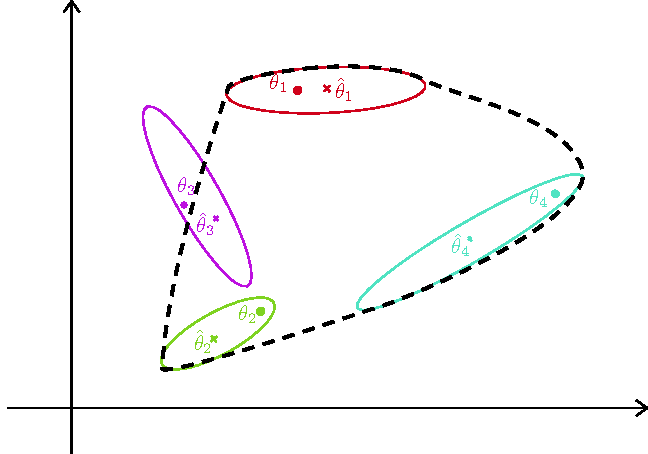
\includegraphics[width=0.5\linewidth]{sections/appendix/nips2020-bandits/images/condition_feasibility_acceptance.pdf}
	\caption{Illustrative example of condition \eqref{eq:feasibilty_condition}. The target arm is arm $3$ or $5$ and the dashed black line is the convex hull of the other confidence sets. The ellipsoids are the confidence sets $\mathcal{C}_{t,a}$ for each arm $a$. If we consider only arms $\{1,2,4,5\}$, and we use $5$ as the target arm, the condition \eqref{eq:feasibilty_condition} is satisfied as there is a $\theta$ outside the convex hull of the other confidence sets. On the other hand, if we consider arms $\{1,2,3,4\}$ and we use $3$ as the target arm, the condition is not satisfied anymore. \label{fig:feasibility_condition}}
\end{figure}

\changebr{Let us assume that \changebrtwo{there is an arm in $a^\dagger\in A^\dagger$ which is} optimal for some contexts. More formally, there exists a subspace $V\subset \mathcal{D}$ such that:} 
\begin{equation*}    
\forall x\in V, \exists a^{\dagger}_{\star}(x)\in A^\dagger, \forall a\in \llbracket 1, K\rrbracket\setminus\{a^{\dagger}_{\star}(x)\} \qquad \langle x, \theta_{a^{\dagger}_{\star}(x)}\rangle > \left\langle x, \theta_{a}\right\rangle.
\end{equation*}
\changebr{We also assume that} the distribution of the contexts is such that, for all $t$, $\mu := \mathbb{P}\left(x_{t}\in V\right) >0$.
Then\changebr{,} the regret is lower-bounded in expectation by:
\begin{align*}
    \mathbb{E}(R_{T}) &= \mathbb{E}\left(\sum_{t=1}^{T} \mathds{1}_{\{x_{t}\in V\}}\big( \left\langle x_{t}, \theta_{a^{\dagger}_{\star}(x_{t})} - \theta_{a_{t}}\right\rangle\big)\right) \geq \mu m(T) \min_{x\in V} \max_{a\neq a^{\dagger}_\star(x)} \langle \theta_{a^{\dagger}_{\star}(x)} - \theta_{a}, x\rangle
\end{align*}
where $m(T)$ is the expected number of times $t\leq T$ such that condition \eqref{eq:feasibilty_condition} is not met. \changebr{\linucb guarantees that}  $\mathbb{E}(R_{T}) \leq \mathcal{O}(\sqrt{T})$ for every $T$. Hence, 
\begin{align*}
    m(T) \leq \mathcal{O}\left(\frac{\sqrt{T}}{\mu\min_{x\in V}\max_{a\neq a^{\dagger}_\star(x)} \langle \theta_{a^{\dagger}_{\star}(x)} - \theta_{a}, x\rangle}\right)
\end{align*}
This means that, in an unattacked problem, condition \eqref{eq:feasibilty_condition} is met $T - \mathcal{O}(\sqrt{T})$ times. On the other hand, when the algorithm is attacked the regret of \linucb is not sub-linear as the confidence bound for the target arm is not valid anymore. Hence we cannot provide the same type of guarantees for the attacked problem.



% !TEX root = main.tex
\section{Experiments}

\subsection{Datasets and preprocessing}\label{app:experiments_setup}
% \todoe{This section also explain how we preprocessed the real-wolrd datasets too.}

We present here the datasets used in the article and how we preprocess them for numerical experiments conducted in Section \ref{sec:experiments}.

We consider two types of experiments, one on synthetic data with a contextual MAB problems with $K = 10$ arms such that for every arm $a$, $\theta_{a}$ is drawn from a folded normal distribution in dimension $d = 30$. We also use a finite number of contexts ($10$), each of them is drawn from a folded normal distribution projected on the unit circle multiplied by a uniform radius variable (i.i.d. across all contexts). Finally, we scale the expected rewards in $(0,1]$ and the noise is drawn from a centered Gaussian distribution $\mathcal{N}(0, 0.01)$. 
% The target arm is chosen at random among all arms. %I removed it because this is not always true 

The second type of experiments is conducted in the real-world datasets Jester \cite{goldberg2001eigentaste} and MovieLens25M \cite{harper2015movielens}. Jester consists of joke ratings on a continuous scale from $-10$ to $10$ for $100$ jokes from a total of $73421$ users. We use the features extracted via a low-rank matrix factorization ($d = 35$) to represent the actions (i.e., the jokes). We consider a complete subset of $40$ jokes and $19181$ users . Each user  rates all the $40$ jokes. At each time, a user is randomly selected from the $19181$ users and mean rewards are normalized in $[0, 1]$. The reward noise is $\mathcal{N} (0, 0.01)$. The second dataset we use is MovieLens25M. It contains $25000095$ ratings created by $162541$ users on $62423$ movies. We perform a low-rank matrix factorization to compute users features and movies features. We keep only movies with at least $1000$ ratings, which leave us with $162539$ users and $3794$ movies. At each time step, we present a random user, and the reward is the scalar product between the user feature and the recommend movie feature. All rewards are scaled to lie in $[0,1]$ and a Gaussian noise $\mathcal{N}(0, 0.01)$ is added to the rewards. 


\subsection{Attacks on Rewards}\label{app:additional_fig_rwds}
In this appendix, we present empirical evolution of the total cost and the number of draws for a unique target arm as a function of the attack parameter $\gamma$ for the Contextual ACE attack with perturbed rewards $\tilde{r}^{2}$ on generated data.

\begin{figure}[htbp]
    \centering
    \subfigure[Total cost]{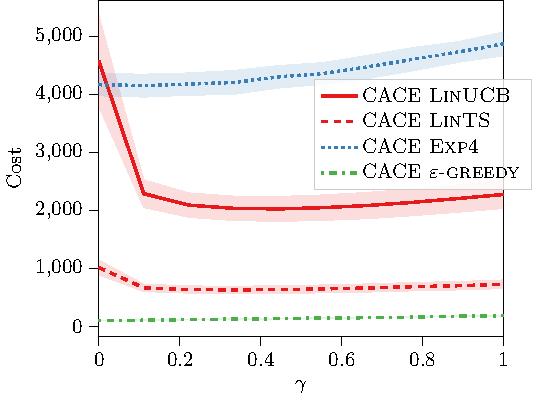
\includegraphics[width=0.35\textwidth]{images/attack_reward/simulations/cost_epsilon.pdf}}
    \subfigure[Number of draws]{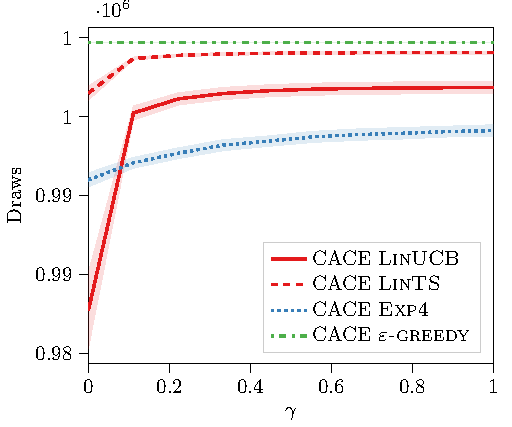
\includegraphics[width=0.3\textwidth]{images/attack_reward/simulations/draws_epsilon.pdf}}
    \caption{Total cost of attacks and number of draws of the target arm at $T = 10^{6}$ as a function of $\gamma$ on synthetic data}
    \label{fig:synth_cost_draws_gamma}
\end{figure}

Fig.~\ref{fig:synth_cost_draws_gamma} (left) shows that the total cost of attacks seems to be quite invariant w.r.t.  $\gamma$ except when $\gamma \rightarrow 0$ because the difference between the target arm and the other becomes negligible. This is also depicted by the total number of draws (Fig.~\ref{fig:synth_cost_draws_gamma}, Right) as the number of draws plummets when $\gamma \rightarrow 0$.

\begin{table}
\begin{center}
	\caption{\label{table:number_of_draws}Number of draws of the target arm $a^{\dagger}$ at $T=10^{6}$, for the synthetic data, $\gamma = 0.22$ for the Contextual ACE algorithm and for the Jester and MovieLens datasets $\gamma = 0.5$\otc{.}}
\begin{tabular}{lccc}
\toprule
{} & Synthetic &  Jester & Movilens \\
\midrule
\linucb          &      $86, 731.6$ &  $23, 548.16$ &    $25, 017.31$ \\
CACE \linucb     &     $996, 238.6$ &  $921, 083.69$ &   $944, 721.28$ \\
Stationary CACE \linucb &     $995, 578.88$ & $862, 095.67$ &   $931, 531.6$ \\
\epsgreedy       &     $111, 380.44$ & $21, 911.54$ &    $3, 165.81$    \\
CACE \epsgreedy  &    $999, 812.92$ &  $999, 755.72$ &   $999, 776.82$ \\
Stationary CACE \epsgreedy &     $999, 806.32$ &  $999, 615.98$ &   $999, 316.76$ \\
\lints           &      $91, 664.8$ &  $23, 398.3$ &    $30, 189.84$ \\
CACE \lints      &      $998, 997.04$ &   $976, 708.9$ &   $990, 250.67$ \\
Stationary CACE \lints &     $977, 850.96$ & $784, 715.62$ &   $845, 512.98$ \\
\expfour         &     $93, 860.4$ &  $29, 147.01$ &    $17, 985.78$ \\
CACE \expfour    &    $992, 793.36$ &   $989, 214.36$ &    $936, 230.4$ \\
Stationary CACE \expfour &     $993, 673.24$ &  $988, 463.56$ &   $934, 304.23$ \\
\bottomrule
\end{tabular}

\end{center}
\end{table}

\subsection{Attacks on all Contexts}\label{app:additional_fig_all_ctx}

% \begin{figure}[h]
%     \centering
%     \subfigure[Synthetic data]{\includegraphics[width=0.33\textwidth]{images/all_context_3_alg_sim/gen_cost_all.pdf}}\hfill
%     \subfigure[Jester Dataset]{\includegraphics[width=0.23\textwidth]{images/all_contexts_3_algs_jester/gen_jester_cost_all.pdf}}\hfill
%     \subfigure[MovieLens Dataset]{\includegraphics[width=0.23\textwidth]{images/all_contexts_3_alg_movielens/gen_movielens_cost_all.pdf}}
%     \caption{Total cost of the attacks for the attack of Sec.~\ref{sec:attack_all_context} on our synthetic dataset, Jester and MovieLens}
%     \label{fig:cost_all_algs_attack_all_ctx}
% \end{figure}

% Fig.~\ref{fig:cost_all_algs_attack_all_ctx} shows the total cost for all the attacks (that is to say including CC \lints and CC$20$ \lints compared to Fig~\ref{fig:costs_plot} (Right)). This figure shows that even though the total cost of attacks is linear for the synthetic and Jester dataset, it seems that for MovieLens the attacker achieves their goal with a logarithmic total. Therefore, despite the fact that the estimate of $\theta_{a^\dagger}$ can be polluted by attacked samples, it seems that \lints can still pick up $a^{\dagger}$ as being optimal for this particular instance.

\begin{figure}[h]
   \begin{minipage}{0.25\linewidth}
        \centering
        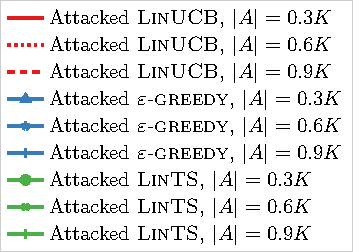
\includegraphics[width=0.85\linewidth]{images/regret_cost_attacks_context/simulations/legend.pdf}
        %\caption{Lorem ipsum}
    \end{minipage}\hfill
    \begin{minipage}{0.25\linewidth}
    \centering
    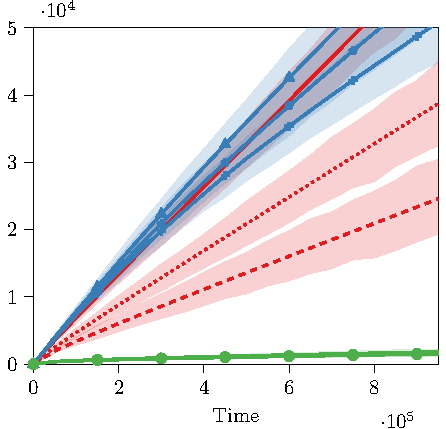
\includegraphics[width=0.95\linewidth]{images/regret_cost_attacks_context/simulations/standalone.pdf}
    % \caption{Synthetic}
    \end{minipage}\hfill
    \begin{minipage}{0.25\linewidth}
    \centering
    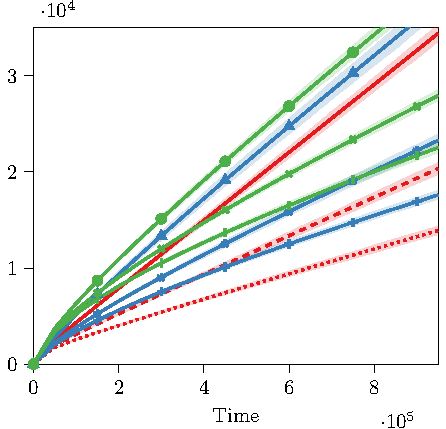
\includegraphics[width=0.85\linewidth]{images/regret_cost_attacks_context/jester/standalone.pdf}
    % \caption{Jester}
    \end{minipage}\hfill
    \begin{minipage}{0.25\linewidth}
    \centering
    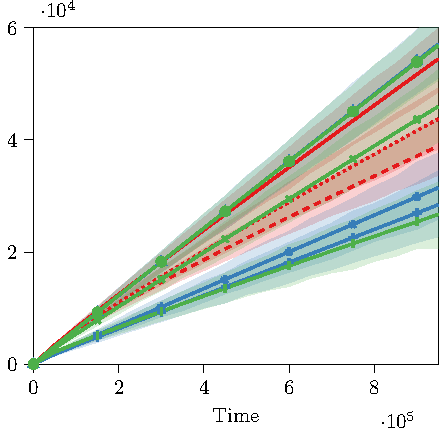
\includegraphics[width=0.85\linewidth]{images/regret_cost_attacks_context/movielens/standalone.pdf}
    % \caption{MovieLens}
    \end{minipage}
    \label{fig:regret_all_algs_attack_all_ctx}
\end{figure}

Fig.~\ref{fig:regret_all_algs_attack_all_ctx} shows the regret for all the attacks. This figure shows that even though the total cost of attacks is linear for algorithms like \lints in the synthetic dataset, the regret is linear. More generally, we observe that the regret is linear for all attacked algorithms on all datasets.

\subsection{Attack on a single context}\label{app:additional_fig_one_ctx}

The attacks are computed by solving the optimization problems \ref{eq:attack_one_user} and \ref{eq:relaxed_attack_one_user} (Sec.~\ref{sec:attack_one_context}). We choose the libraries according to their efficiency for each problem we need to solve. For Problem \eqref{eq:relaxed_attack_one_user} and Problem \eqref{eq:relaxed_TS_attack_one_user} we use \textsc{cvxpy}  \cite{cvxpy_rewriting} and the \textsc{ECOS} solver. %to solve the convex relaxations of the optimization problems for \linucb and \lints (equations \ref{eq:relaxed_attack_one_user}, \ref{eq:relaxed_TS_attack_one_user})
For Problem \eqref{eq:attack_one_user} we use the \textsc{SLSQP} method from the Scipy optimize library \cite{scipy} to solve the full \linucb problem (Equation \ref{eq:attack_one_user}) and \textsc{quadprog} to solve the quadratic problem to attack \epsgreedy.


\begin{figure}[htbp]
    \centering
    \subfigure[Synthetic data]{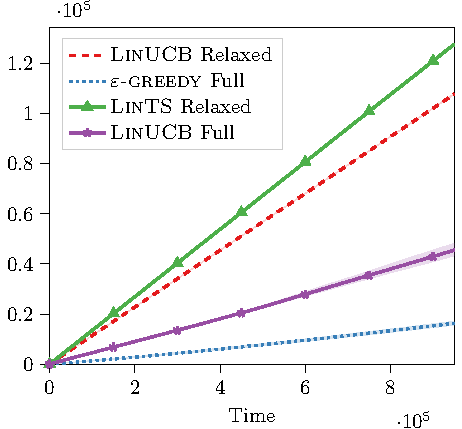
\includegraphics[width=0.33\textwidth]{images/one_context/simulations/standalone.pdf}}\hfill
    \subfigure[Jester Dataset]{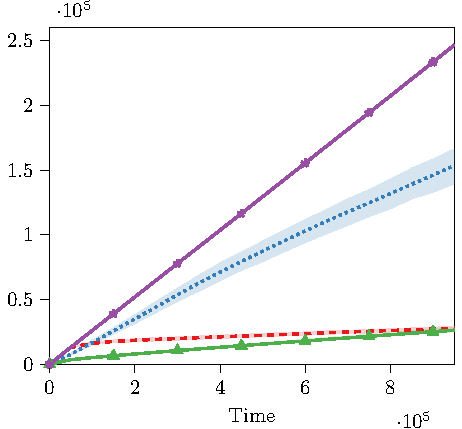
\includegraphics[width=0.33\textwidth]{images/one_context/jester/standalone.pdf}}\hfill
    \subfigure[MovieLens Dataset]{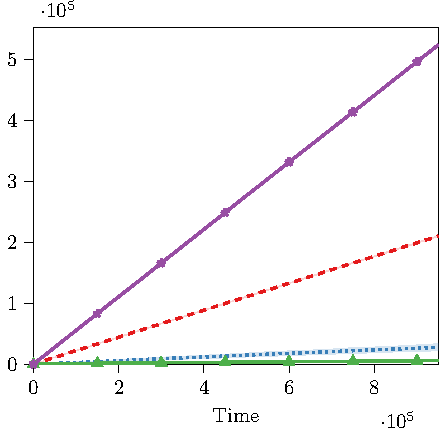
\includegraphics[width=0.33\textwidth]{images/one_context/movielens/standalone.pdf}}
    \caption{Total cost of the attacks for the attacks one one context on our synthetic dataset, Jester and MovieLens. As expected, the total cost is linear.}
    \label{fig:cost_attack_one_ctx}
\end{figure}
% !TEX root = main.tex
\section{Problem \eqref{eq:relaxed_TS_attack_one_user} as a Second Order Cone (SOC) Program}\label{app:one_context_ts_linucb}
Problem \eqref{eq:relaxed_attack_one_user} and Problem \eqref{eq:relaxed_TS_attack_one_user} are both SOC programs. We can see the similarities between both problems as follows. Let us define for every arm \changee{$a\not\in A^{\dagger}$}, the ellipsoid:

$$\mathcal{C}_{t,a}^{'} := \Big\{ y \in \mathbb{R}^{d} \mid || y - \hat{\theta}_{a}(t)||_{A_{a}^{-1}(t)} \leq \upsilon\Phi^{-1}\left( 1 - \frac{\delta}{K-|A^{\dagger}|}\right)\Big\}$$

with $A_{a}(t) = \tilde{V}_{a}^{-1}(t) + \tilde{V}_{a^{\dagger}}^{-1}(t)$ with $\tilde{V}_{a}(t)$ and $\tilde{V}_{a^{\dagger}}(t)$ the design matrix built by \lints and $\hat{\theta}_{a}(t)$ the least squares estimate of $\theta_a$ at time $t$. Therefore for an arm $a$, the constraint in Problem \eqref{eq:relaxed_TS_attack_one_user} can be written for any $y\in\mathbb{R}^{d}$ and some arm $a^{\dagger}\in A^{\dagger}$ as:
\begin{align*}
    \left\langle x^{\star}+y, \hat{\theta}_{a^{\dagger}}(t)\right\rangle - \xi \geq \max_{z\in \mathcal{C}_{t,a}^{'}} \left\langle z, x^{\star} + y\right\rangle
\end{align*}
Indeed for any $x\in \mathbb{R}^{d}$,
\begin{align*}
    \max_{y\in \mathcal{C}_{t,a}^{'}} \left\langle y,x\right\rangle &= \left\langle x, \hat{\theta}_{a}(t)\right\rangle + \upsilon\Phi^{-1}\left( 1 - \frac{\delta}{K-|A^{\dagger}|}\right)\times\max_{ ||A_{a}^{-1/2}(t)u||_{2}\leq 1} \left\langle u, x\right\rangle\\
    &= \left\langle x, \hat{\theta}_{a}(t)\right\rangle + \upsilon\Phi^{-1}\left( 1 - \frac{\delta}{K-|A^{\dagger}|}\right)\max_{ ||z||_{2}\leq 1} \left\langle z, A_{a}^{1/2}(t)x\right\rangle \\
    &= \left\langle x, \hat{\theta}_{a}(t)\right\rangle + \upsilon\Phi^{-1}\left( 1 - \frac{\delta}{K-|A^{\dagger}|}\right)\lVert A_{a}^{1/2}(t)x\rVert_{2}
\end{align*}
Thus, the constraint is feasible if and only if:
\begin{align*}
    \hat{\theta}_{a^{\dagger}}(t) \not\in \text{Conv}\left( \bigcup_{a\not\in A^{\dagger}}  \mathcal{C}_{t,a}^{'}\right)
\end{align*}

\section{Appendix: Attacks on Adversarial Bandits}\label{app:adversarial_rewards}
In the previous sections, we studied algorithms with sublinear regret $R_T$, \ie mainly bandit algorithms designed for stochastic stationary environments. Adversarial algorithms like \expfour do not provably \otc{enjoy} a \changee{sublinear \textbf{stochastic} regret $R_{T}$ (as defined in the introduction) \footnote{\expfour enjoys a sublinear hindsight regret though. Showing a sublinear upper-bound for the stochastic regret of \expfour is still an open problem (see Section $29.1$ in \cite{lattimore2018bandit})}}. In addition, because this type of algorithms are, by design, robust to non-stationary environments, one could expect them to induce a linear cost on the attacker. In this section, we show that this is not the case for most contextual adversarial algorithms. Contextual adversarial algorithms are studied through the reduction to the bandit with expert advice problem. This is a bandit problem with $K$ arms where at every step, $N$ experts suggest a probability distribution over the arms. The goal of the algorithm is to learn which expert gets the best expected reward in hindsight after $T$ steps. The regret in this type of problem is defined as $R_{T}^{\text{exp}} = \mathbb{E}\left( \max_{m\in \llbracket 1, N \rrbracket}\sum_{t=1}^{T} \sum_{j=1}^{K} E_{m,j}^{(t)}r_{t,j} - r_{t,a_{t}}\right)$
% \begin{equation*}
% R_{T}^{\text{exp}} = \mathbb{E}\left( \max_{m\in \llbracket 1, N \rrbracket}\sum_{t=1}^{T} \sum_{j=1}^{K} E_{m,j}^{(t)}r_{t,j} - r_{t,a_{t}}\right)
% \end{equation*} 
where $E_{m,j}^{(t)}$ is the probability of selecting arm $j$ for expert $m$. In the case of contextual adversarial bandit\changebr{s}, the experts first observe the context $x_{t}$ before recommending an expert $m$. 
% In the setting studied in \otc{the present paper, we assume that the rewards are linear. However, defining  a no-regret, similar to the stochastic regret, algorithm for adversarial bandit with this assumption is still an open problem\cite{lattimore2018bandit}.}
% \todobr{I'm not sure I understand this sentence. Does it mean that getting a sublinear regret for linear adversarial bandits is an open problem ? 
% Should we say: In our setting, we assume that the rewards are linear. Finding an sublinear-regret algorithm for adversarial bandits in this setting is still an open problem \cite{lattimore2018bandit}.}
Assuming the current setting with linear rewards, we can show that if an algorithm $\mathfrak{A}$, like \expfour, enjoys a sublinear regret $R_{T}^{\text{exp}}$, then, using the Contextual ACE attack with either $\tilde{r}^{1}$ or $\tilde{r}^{2}$, the attacker can fool the algorithm into pulling arm $a^{\dagger}$ a linear number of times under some \otc{mild} assumptions. However, attacking contexts for this type of algorithm is difficult because, even though the rewards are linear, the experts are not assumed to use a specific model for selecting an action.

% However, for contextual adversarial algorithms like \expfour the regret is not defined in the same way. But through the reduction to bandit with expert advice. Where 
% Proposition \ref{prop:reward_attack} assumes that the regret $R_{T}$ of algorithm $\mathfrak{A}$ is of order $o(T)$ which excludes adversarial algorithms in like \expfour. However, it does not mean that adversarial algorithms are robust to adversarial attacks similar to Contextual ACE. Indeed, for contextual adversarial algorithms the regret is defined through a reduction to bandit with expert advice where at each step a context is presented to a set of $N$ policies and the bandit algorithm has to find the best policy in hindsight after $T$ steps. In that case, the regret is defined as:

% By assuming that to be in the same setting as previously, that is to say for all arms $a$, the reward for arm $a$ is $\langle \theta_{a}, x_{t}\rangle + \eta_{t}$, we can show a similar result concerning the number of times arm $a^{\dagger}$ is pulled as in proposition \ref{prop:rewards_attack} using Contextual ACE with either $\tilde{r}^{1}$ or $\tilde{r}^{2}$ as adversarial algorithms can adapt to no-stationary reward processes.
%\todol{Explain the condition on the expert}
\begin{prop}\label{prop:rwd_attack_adv}
	Suppose an adversarial algorithm $\mathfrak{A}$ satisfies a regret $R_{T}^{\exp}$ of order $o(T)$ for any bandit problem and that there exists an expert $m^{\star}$ such that $ T - \sum_{t=1}^{T} \mathbb{E}\left(E^{(t)}_{m^{\star}, a_{t,\star}^{\dagger}}\right) = o(T)$ with $a_{t,\star}^{\dagger}$ the optimal arim in $A^{\dagger}$ at time $t$. Then attacking alg. $\mathfrak{A}$ with Contextual ACE leads to pulling arm $a^{\dagger}$, $T-o(T)$ of times in expectation with a total cost of $o(T)$ for the attacker.
\end{prop}

\begin{proof}
Similarly to the proof of Proposition \ref{prop:reward_attack}, let's define the bandit with expert advice problem, $\mathcal{A}_{i}$, such that at each time $t$ the reward vector is $(\tilde{r}^{i}_{t,a})_{a}$ (with $i\in\{1, 2\}$). The regret of this algorithm is: $\Tilde{R}_{T}^{i,\text{exp}} = \mathbb{E}\left( \max_{m\in \llbracket 1, N \rrbracket}\sum_{t=1}^{T} E_{m}^{(t)}\Tilde{r}^i_{t} - \Tilde{r}^i_{t,a_{t}}\right)\in o(T)$. The regret of the learner is: $\mathbb{E}\left( \max_{m\in \llbracket 1, N \rrbracket}\sum_{t=1}^{T} E_{m}^{(t)}r_{t} - r_{t,a_{t}}\right)$ where $a_t$ are the actions taken by algorithm $\mathcal{A}_i$ to minimize $\Tilde{R}_{T}^{i,\text{exp}}$. Then we have:
\begin{align*}
    \Tilde{R}_{T}^{i,\text{exp}} \geq \mathbb{E}\left(\sum_{t=1}^{T}\sum_{j=1}^{K} (E_{m^{\star}, j}^{(t)} - \mathds{1}_{\{\changee{j = a_{t,\star}^{\dagger}}\}})\tilde{r}_{t,j}^{i} + \sum_{t=1}^{T} \tilde{r}^{i}_{t, a^{\dagger}_{t,\star}} - \tilde{r}^{i}_{t,a_{t}} \right)
\end{align*}
Therefore, 
\begin{align*}
  \mathbb{E}\left(\sum_{t=1}^{T} \tilde{r}^{i}_{t, a^{\dagger}_{t, \star}} - \tilde{r}^{i}_{t,a_{t}} \right) &\leq \Tilde{R}_{T}^{i,\text{exp}} + \mathbb{E}\left(\sum_{t=1}^{T}\sum_{j=1}^{K} (\mathds{1}_{\{\changee{j = a_{t,\star}^{\dagger}}\}} - E_{m^{\star}, j}^{(t)})\tilde{r}_{t,j}^{i}\right) \\
  &\leq \Tilde{R}_{T}^{i,\text{exp}} + \mathbb{E}\left(\sum_{t=1}^{T}(1 - E_{m^{\star}, a^{\dagger}_{t,\star}}^{(t)})\tilde{r}_{t,j}^{i}\right) \\
  &\leq \Tilde{R}_{T}^{i,\text{exp}} + \mathbb{E}\left(\sum_{t=1}^{T}(1 - E_{m^{\star}, a^{\dagger}_{t,\star}}^{(t)})\right)
\end{align*}

For strategy $i=1$, we have:
\begin{align*}
    \mathbb{E}\left(\sum_{t=1}^{T} \tilde{r}^{1}_{t, a^{\dagger}_{t, \star}} - \tilde{r}^{1}_{t,a_{t}} \right) &=
    \changee{\sum_{t=1}^{T} \mathbb{E}\left(r_{t,a_{t,\star}^{\dagger}} - \mathds{1}_{\{ a_{t}\in A^{\dagger}\}}\right)\geq \left(T-\mathbb{E}\left(\sum_{t=1}^{T} \mathds{1}_{\{ a_{t} = a_{t,\star}^{\dagger}\}}\right)\right)\Delta}
\end{align*}
\changee{where $\Delta := \min_{x\in \mathcal{D}}\left\{ \langle \theta_{a^\dagger(x)}, x\rangle - \max_{a\in A^{\dagger},a\neq a^{\dagger}(x)} \langle \theta_{a'}, x\rangle\right\}$ with $a^{\dagger}(x) := \arg\max_{a\in A^{\dagger}} \langle \theta_{a}, x\rangle$}. Then, as $\Tilde{R}_{T}^{1,\text{exp}}\in o(T)$ and $\mathbb{E}\left(\sum_{t=1}^{T}(1 - E_{m^{\star}, a^{\dagger}_{t, \star}}^{(t)})\right)\in o(T)$, we deduce that
\begin{align*}
    \mathbb{E}(\sum_{t} \mathds{1}_{\{ a_{t} = a_{t,\star}
^{\dagger}\}}) = T-o(T)\quad.
\end{align*}

% For this strategy the cost is therefore bounded by: 
% \begin{align*}
% \mathbb{E}\left( \sum_{t=1}^{T} c_{t}\right) &\leq \mathbb{E}\left(\sum_{t=1}^{T} \mathds{1}_{\{a_{t}\neq a^{\dagger}\}} + |\eta_{a_{t}, t}|+ |\eta_{a_{t},t}'|\right) \leq (1 + 2\sigma) \mathbb{E}\left( N_{a^{\dagger}}(T)\right)
% \end{align*}

For strategy $i=2$, and $\delta>0$, let us denote by $E_{\delta}$ the event that all confidence intervals hold with probability $1 - \delta$. But on the event $E_{\delta}$, for a time $t$ where $a_{t}\neq a^{\dagger}_{t,\star}$ and such that $-1\leq C_{t,a_{t}} \leq 0$:
\begin{align*}
\tilde{r}^{2}_{t,a_{t}} = r_{t, a_{t}} + C_{t,a_{t}} &= (1 - \gamma)\min_{a^{\dagger}\in A^{\dagger}} \min_{\theta\in \mathcal{C}_{t,a^{\dagger}}} \langle \theta, x_{t}\rangle + \eta_{a_{t},t} + \langle\theta_{a}, x_{t}\rangle - \max_{\theta\in \mathcal{C}_{t,a_{t}}} \langle \theta, x_{t}\rangle \\
&\leq (1 - \gamma) \langle \theta_{a^{\dagger}_{t,\star}}, x_{t}\rangle + \eta_{a_{t},t}
\end{align*}
when $C_{t,a_{t}} >0$ (still on the event $E_{\delta}$):
\begin{align*}
\tilde{r}^{2}_{t,a_{t}} = r_{t,a_{t}} \leq (1 - \gamma) \langle \theta_{a^{\dagger}_{t,\star}}, x_{t}\rangle + \eta_{a_{t},t}
\end{align*}
because $C_{t,a_{t}}>0$ means that $(1 - \gamma) \langle \theta_{a^{\dagger}_{t,\star}}, x_{t}\rangle \geq (1 - \gamma)\min_{a^{\dagger}\in A^{\dagger}}\min_{\theta\in \mathcal{C}_{t,a^{\dagger}}} \langle \theta, x_{t}\rangle \geq \max_{\theta\in \mathcal{C}_{t,a_{t}}} \langle \theta, x_{t}\rangle \geq \langle \theta_{a}, x_{t}\rangle$. But finally, when $C_{t,a_{t}} \leq -1$, $\tilde{r}^{2}_{t,a_{t}} = r_{t,a_{t}} -1 \leq \eta_{a_{t},t} \leq (1- \gamma)\langle \theta_{a^{\dagger}_{t,\star}}, x_{t}\rangle + \eta_{a_{t},t}$.  But on the complementary event $E_{\delta}^{c}$,  $ \tilde{r}^{2}_{t,a_{t}} \leq r_{t,a_t}$. Thus, given that the expected reward is assumed to be bounded in $(0,1]$ (Assumption~\ref{assumption1}):
\begin{align*}
    \mathbb{E}\left(\sum_{t=1}^{T} \tilde{r}^{2}_{t, a^{\dagger}_{t,\star}} - \tilde{r}^{2}_{t,a_{t}} \right) & =  \mathbb{E}\left(\sum_{t=1}^{T} (r_{t, a^{\dagger}} - \tilde{r}^{2}_{t,a_{t}})\mathds{1}_{\{a_{t}\neq a^{\dagger}_{t,\star}\}} \right) \\
    &\geq \mathbb{E}\left(\sum_{t=1}^{T} \min\{\gamma\min_{x\in\mathcal{D}} \langle x, \theta_{a^{\dagger}_{t,\star}}\rangle, \Delta\} \mathds{1}_{\{a_{t}\neq a^{\dagger}_{t,\star}\}}\mathds{1}_{\{E_{\delta}\}}\right)-T\delta
\end{align*}
Finally, putting everything together we have:
\begin{align*}
    \mathbb{E}&\left(\sum_{t=1}^{T} \gamma\min_{x\in\mathcal{D}} \langle x, \theta_{a^{\dagger}_{t,\star}}\rangle \mathds{1}_{\{a_{t}\neq a^{\dagger}_{t,\star}\}}\right) \leq &\Tilde{R}_{T}^{2,\text{exp}} + \mathbb{E}\left(\sum_{t=1}^{T}(1 - E_{m^{\star}, a^{\dagger}_{t,\star}}^{(t)})\right)\\
     &+ \delta T \left(\min\{\gamma\min_{a^{\dagger}\in A^{\dagger}}\min_{x\in\mathcal{D}} \langle x, \theta_{a^{\dagger}}\rangle, \Delta\} +1\right)
\end{align*}
Hence, because $\Tilde{R}_{T}^{1,\text{exp}} = o(T)$ and $\mathbb{E}\left(\sum_{t=1}^{T}(1 - E_{m^{\star}, a^{\dagger}}^{(t)})\right) = o(T)$ we have that for $\delta \leq 1/T$, the expected number of pulls of the optimal arm in $A^{\dagger}$ is of order $o(T)$. In addition, the cost for the attacker is bounded by: 
\begin{align*}
\mathbb{E}\left(\sum_{t=1}^{T} c_{t}\right) &= \mathbb{E}\left(\sum_{t=1}^{T} \mathds{1}_{\{a_{t}\neq a^{\dagger}_{t,\star}\}} \big|\max(-1, \min(C_{t, a_{t}},0))\big| \right)\leq  \mathbb{E}\left( \sum_{t=1}^{T} \mathds{1}_{\{a_{t}\neq a^{\dagger}_{t,\star}\}}\right)
\end{align*}
\end{proof}

The proof is similar to the one of Prop.~\ref{prop:reward_attack}. The condition on the expert in Prop.~\ref{prop:rwd_attack_adv} means that there exists an expert which believes an arm $a^{\dagger}\in A^{\dagger}$ is optimal most of the time. The adversarial algorithm will then learn that this expert is optimal. %The rewards presented to the algorithm are build in such a way that the latter learns that the expert pulling arm $a^{\dagger}$ the majority of times being optimal.% \begin{proof}
% Similarly to the proof of Proposition \ref{prop:reward_attack}, let's define the bandit with expert advice problem, $\mathcal{A}_{i}$, such that at each time $t$ the reward vector is $(\tilde{r}^{i}_{t,a})_{a}$ (with $i\in\{1, 2\}$). The regret of this algorithm is: $\Tilde{R}_{T}^{i,\text{exp}} = \mathbb{E}\left( \max_{m\in \llbracket 1, N \rrbracket}\sum_{t=1}^{T} E_{m}^{(t)}\Tilde{r}^i_{t} - \Tilde{r}^i_{t,a_{t}}\right)\in o(T)$. The regret of the learner is: $\mathbb{E}\left( \max_{m\in \llbracket 1, N \rrbracket}\sum_{t=1}^{T} E_{m}^{(t)}r_{t} - r_{t,a_{t}}\right)$ where $a_t$ are the actions taken by algorithm $\mathcal{A}_i$ to minimize $\Tilde{R}_{T}^{i,\text{exp}}$. Then we have:
% \begin{align*}
%     \Tilde{R}_{T}^{i,\text{exp}} \geq \mathbb{E}\left(\sum_{t=1}^{T}\sum_{j=1}^{K} (E_{m^{\star}, j}^{(t)} - \mathds{1}_{\{j\neq a^{\dagger}\}})\tilde{r}_{t,j}^{i} + \sum_{t=1}^{T} \tilde{r}^{i}_{t, a^{\dagger}} - \tilde{r}^{i}_{t,a_{t}} \right)
% \end{align*}
% Therefore, 
% \begin{align*}
%   \mathbb{E}\left(\sum_{t=1}^{T} \tilde{r}^{i}_{t, a^{\dagger}} - \tilde{r}^{i}_{t,a_{t}} \right) &\leq \Tilde{R}_{T}^{i,\text{exp}} + \mathbb{E}\left(\sum_{t=1}^{T}\sum_{j=1}^{K} (\mathds{1}_{\{j\neq a^{\dagger}\}} - E_{m^{\star}, j}^{(t)})\tilde{r}_{t,j}^{i}\right) \\
%   &\leq \Tilde{R}_{T}^{i,\text{exp}} + \mathbb{E}\left(\sum_{t=1}^{T}(1 - E_{m^{\star}, a^{\dagger}}^{(t)})\tilde{r}_{t,j}^{i}\right) \\
%   &\leq \Tilde{R}_{T}^{i,\text{exp}} + \mathbb{E}\left(\sum_{t=1}^{T}(1 - E_{m^{\star}, a^{\dagger}}^{(t)})\right)
% \end{align*}
% For strategy $i=1$, and $\delta>0$, let denote $E_{\delta}$ the event that all confidence intervals holds with probability $1 - \delta$. But on the event $E_{\delta}$, for a time $t$ where $a_{t}\neq a^{\dagger}$ and such that $-1\leq C_{t,a_{t}} \leq 0$:
% \begin{align*}
% \tilde{r}^{1}_{t,a_{t}} = r_{t, a_{t}} + C_{t,a_{t}} &= (1 - \gamma) \min_{\theta\in \mathcal{C}_{t,,a^{\dagger}}} \langle \theta, x_{t}\rangle + \eta_{a_{t},t} + \langle\theta_{a}, x_{t}\rangle - \max_{\theta\in \mathcal{C}_{t,a_{t}}} \langle \theta, x_{t}\rangle \\
% &\leq (1 - \gamma) \langle \theta_{a^{\dagger}}, x_{t}\rangle + \eta_{a_{t},t}
% \end{align*}
% when $C_{t,a_{t}} >0$ (still on the event $E_{\delta}$):
% \begin{align*}
% \tilde{r}^{1}_{t,a_{t}} = r_{t,a_{t}} \leq (1 - \gamma) \langle \theta_{a^{\dagger}}, x_{t}\rangle + \eta_{a_{t},t}
% \end{align*}
% because $C_{t,a_{t}}>0$ means that $(1 - \gamma) \langle \theta_{a^{\dagger}}, x_{t}\rangle \geq (1 - \gamma)\min_{\theta\in \mathcal{C}_{t,,a^{\dagger}}} \langle \theta, x_{t}\rangle \geq \max_{\theta\in \mathcal{C}_{t,a_{t}}} \langle \theta, x_{t}\rangle \geq \langle \theta_{a}, x_{t}\rangle$. But finally, when $C_{t,a_{t}} \leq -1$, $\tilde{r}^{1}_{t,a_{t}} = r_{t,a_{t}} -1 \leq \eta_{a_{t},t} \leq (1- \gamma)\langle \theta_{a^{\dagger}}, x_{t}\rangle + \eta_{a_{t},t}  $.  But on the complementary event $E_{\delta}^{c}$,  $ \tilde{r}^{1}_{t,a_{t}} \leq r_{t,a_t}$. Thus we have because the expected reward are assumed to be bounded in $(0,1]$:
% \begin{align*}
%     \mathbb{E}\left(\sum_{t=1}^{T} \tilde{r}^{1}_{t, a^{\dagger}} - \tilde{r}^{1}_{t,a_{t}} \right)  =  \mathbb{E}\left(\sum_{t=1}^{T} (r_{t, a^{\dagger}} - \tilde{r}^{1}_{t,a_{t}})\mathds{1}_{\{a_{t}\neq a^{\dagger}\}} \right) &\\
%     \geq \mathbb{E}\left(\sum_{t=1}^{T} \gamma\min_{x\in\mathcal{D}} \langle x, \theta_{a^{\dagger}}\rangle \mathds{1}_{\{a_{t}\neq a^{\dagger}\}}\mathds{1}_{\{E_{\delta}\}}\right)-T\delta
% \end{align*}
% Finally, putting everything together we have:
% \begin{align*}
%     \mathbb{E}&\left(\sum_{t=1}^{T} \gamma\min_{x\in\mathcal{D}} \langle x, \theta_{a^{\dagger}}\rangle \mathds{1}_{\{a_{t}\neq a^{\dagger}\}}\right) \leq \Tilde{R}_{T}^{1,\text{exp}} \\
%     &+ \mathbb{E}\left(\sum_{t=1}^{T}(1 - E_{m^{\star}, a^{\dagger}}^{(t)})\right) + \delta T \left(\gamma\min_{x\in\mathcal{D}} \langle x, \theta_{a^{\dagger}}\rangle +1\right)\\
% \end{align*}
% Hence, because $\Tilde{R}_{T}^{1,\text{exp}} = o(T)$ and $\mathbb{E}\left(\sum_{t=1}^{T}(1 - E_{m^{\star}, a^{\dagger}}^{(t)})\right) = o(T)$ we have that for $\delta \leq 1/T$, the expected number of pulls of arm $a^{\dagger}$ is of order $o(T)$. In addition, the cost for the attacker is bounded by: 
% \begin{align*}
% \mathbb{E}\left(\sum_{t=1}^{T} c_{t}\right) &= \mathbb{E}\left(\sum_{t=1}^{T} \mathds{1}_{\{a_{t}\neq a^{\dagger}\}} \big|\max(-1, \min(C_{t, a_{t}},0))\big| \right)\\
% &\leq  \mathbb{E}\left( \sum_{t=1}^{T} \mathds{1}_{\{a_{t}\neq a^{\dagger}\}}\right)
% \end{align*}
% For strategy $i=2$, we have:
% \begin{align*}
%     \mathbb{E}\left(\sum_{t=1}^{T} \tilde{r}^{2}_{t, a^{\dagger}} - \tilde{r}^{2}_{t,a_{t}} \right) &=
%     \sum_{t=1}^{T} \mathbb{E}\left(r_{t, a^{\dagger}}\mathds{1}_{a_t\neq a^\star}\right)\\
%  &\geq (T-\mathbb{E}(N_{a^\star}(T)))\min_{x\in\mathcal{D}} \langle x, \theta_{a^{\dagger}}\rangle 
% \end{align*}
% Then, as $\Tilde{R}_{T}^{2,\text{exp}}\in o(T)$ and $\mathbb{E}\left(\sum_{t=1}^{T}(1 - E_{m^{\star}, a^{\dagger}}^{(t)})\right)\in o(T)$, we deduce that $\mathbb{E}(N_{a^\star}(T)) = T-o(T)$. For this strategy the cost is bounded by: 
% \begin{align*}
% \mathbb{E}\left( \sum_{t=1}^{T} c_{t}\right) &\leq \mathbb{E}\left(\sum_{t=1}^{T} \mathds{1}_{\{a_{t}\neq a^{\dagger}\}} + |\eta_{a_{t}, t}|+ |\eta_{a_{t},t}'|\right) \\
% &\leq (1 + 2\sigma) \mathbb{E}\left( N_{a^{\dagger}}(T)\right)
% \end{align*}
% \todol{add regret (I have it but need to write) + add details on line 480 col 2}
% \end{proof}
Algorithm \expfour has a regret $R_{T}^{\text{exp}}$ bounded by $\sqrt{2TK\log(N)}$, thus the total number of pulls of arms not in $A^{\dagger}$ %different from $a^{\dagger}$ 
is bounded by $\sqrt{2TK\log(M)}/\gamma$. This result also implies that for adversarial algorithms like \expthree \cite{auer2002finite}, the same type of attacks could be used to fool $\mathfrak{A}$ into pulling arms in $A^{\dagger}$ because the MAB problem can be seen as a reduction of the contextual bandit problem with a unique context and one expert for each arm.

%consisting of the mean of each arm as coordinate and each experts selects only one arm.

% !TEX root = main.tex
\section{Contextual Bandit Algorithms}\label{app:algorithms}

In this appendix, we present the different bandit algorithms studied in this paper. All algorithms we consider except \expfour uses disjoint models for building estimate of the arm feature vectors $(\theta_{a})_{a\in\llbracket 1, K\rrbracket}$. Each algorithm (except \expfour) builds least squares estimates of the arm features.

\begin{algorithm}[h]
  \caption{Contextual \linucb}
  \label{alg:linucb}
\begin{algorithmic}
  \STATE {\bfseries Input:} regularization  $\lambda$, number of arms $K$, number of rounds $T$, bound on context norms: $L$, bound on norms $\theta_{a}$: $D$
  \STATE Initialize for every arm $a$, $\bar{V}_{a}^{-1}(t) = \frac1\lambda I_{d}$, $\hat{\theta}_{a}(t) = 0$ and $b_{a}(t) = 0$
  \FOR{$t=1,..., T$}
  \STATE Observe context $x_{t}$
  \STATE Compute $\beta_{a}(t) = \sigma\sqrt{d\log\left(\frac{1 +  N_{a}(t)L^{2}/\lambda}{\delta}\right)}$ with $N_{a}(t)$ the number of pulls of arm $a$
  \STATE Pull arm  $a_{t} =\argmaxB_a \langle \hat{\theta}_{a}(t),x_t\rangle + \beta_{a}(t)||x_{t}||_{\bar{V}_{a}^{-1}(t)}$
  \STATE Observe reward $r_{t}$ and update parameters $\hat{\theta}_{a}(t)$ and $\bar{V}_{a}^{-1}(t)$ such that:
  \begin{align*}
      \bar{V}_{a_{t}}(t+1) = \bar{V}_{a_{t}}(t) + x_{t}x_{t}^{\intercal},\quad b_{a_{t}}(t+1) = b_{a_{t}}(t) + r_{t}x_{t},\quad\theta_{a_{t}}(t+1) = \bar{V}_{a_{t}}^{-1}(t+1)b_{a_{t}}(t+1)
  \end{align*}
  \ENDFOR
\end{algorithmic}
\end{algorithm}

\begin{algorithm}[h]
  \caption{Linear Thompson Sampling with Gaussian prior}
  \label{alg:linTS}
\begin{algorithmic}
  \STATE {\bfseries Input:} regularization  $\lambda$, number of arms $K$, number of rounds $T$, variance $\upsilon$
  \STATE Initialize for every arm $a$, $\bar{V}_{a}^{-1}(t) = \lambda I_{d}$ and $\hat{\theta}_{a}(t) = 0$, $b_{a}(t) = 0$
  \FOR{$t=1,..., T$}
  \STATE Observe context $x_{t}$
  \STATE Draw $\tilde{\theta}_{a}\sim\mathcal{N}(\hat{\theta}_{a}(t), \upsilon^{2}\bar{V}_{a}^{-1}(t))$
  \STATE Pull arm $a_{t} = \argmaxB_{a\in \llbracket 1, K\rrbracket} \left\langle \tilde{\theta}_{a}, x_{t}\right\rangle$
  \STATE Observe reward $r_{t}$ and update parameters $\hat{\theta}_{a}(t)$ and $\bar{V}_{a}^{-1}(t)$
    \begin{align*}
      \bar{V}_{a_{t}}(t+1) = \bar{V}_{a_{t}}(t) + x_{t}x_{t}^{\intercal},\quad b_{a_{t}}(t+1) = b_{a_{t}}(t) + r_{t}x_{t},\quad\theta_{a_{t}}(t+1) = \bar{V}_{a_{t}}^{-1}(t+1)b_{a_{t}}(t+1)
  \end{align*}
  \ENDFOR
\end{algorithmic}
\end{algorithm}

\begin{algorithm}[h]
  \caption{\epsgreedy}
  \label{alg:egreedy}
\begin{algorithmic}
  \STATE {\bfseries Input:} regularization  $\lambda$, number of arms $K$, number of rounds $T$, exploration parameter $(\varepsilon)_{t}$
	\STATE Initialize, for all arms $a$, $\bar{V}_{a}^{-1}(t) = \lambda I_{d}$ and $\hat{\theta}_{a}(t) = 0$, $\varepsilon_{t} = 1$, $b_{a}(t) = 0$
  \FOR{$t=1,..., T$}
  \STATE Observe context $x_{t}$
  \STATE With probability $\varepsilon_{t}$, pull $a_{t} \sim \mathcal{U}\left(\llbracket 1,K\rrbracket\right)$, or pull $a_{t} = \argmaxB \langle \theta_{a}, x_{t}\rangle$ 
  \STATE Observe reward $r_{t}$ and update parameters $\hat{\theta}_{a}(t)$ and $\bar{V}_{a}^{-1}(t)$
    \begin{align*}
      &\bar{V}_{a_{t}}(t+1) = \bar{V}_{a_{t}}(t) + x_{t}x_{t}^{\intercal},\quad b_{a_{t}}(t+1) = b_{a_{t}}(t) + r_{t}x_{t},\\
      &\theta_{a_{t}}(t+1) = \bar{V}_{a_{t}}^{-1}(t+1)b_{a_{t}}(t+1)
  \end{align*}
  \ENDFOR
\end{algorithmic}
\end{algorithm}

\begin{algorithm}[h]
  \caption{\expfour}
  \label{alg:exp4}
\begin{algorithmic}
	\STATE {\bfseries Input:} number of arms $K$, experts: $(E_{m})_{m\in\llbracket 1, N\rrbracket}$, parameter $\eta$
  \STATE Set $Q_{1} = (1/N)_{j\in\llbracket 1, N\rrbracket}$
  \FOR{$t=1,..., T$}
  \STATE Observe context $x_{t}$ and probability recommendation $(E_{m}^{(t)})_{m\in\llbracket 1, N\rrbracket}$
  \STATE Pull arm $a_{t}\sim P_{t}$ where $P_{t,j} = \sum_{k=1}^{N} Q_{t,k}E_{j,k}^{(t)}$ 
  \STATE Observe reward $r_{t}$ and define for all arms $i$ $\hat{r}_{t,i} = 1 - \mathds{1}_{\{ a_{t}=i\}}( 1 - r_{t})/P_{t,i}$
  \STATE Define $\tilde{X}_{t,k} = \sum_{a} E_{k, a}^{(t)}\hat{r}_{t,a}$
  \STATE Update $Q_{t+1, j} = \exp(\eta Q_{t,i})/\sum_{j=1}^{N} \exp(\eta Q_{t,j})$ for all experts $i$
  \ENDFOR
\end{algorithmic}
\end{algorithm}

% !TEX root = main.tex
\section{Semi-Online Attacks}

\cite{liu2019data} studies what they call the offline setting for adversarial attacks on stochastic bandits. They consider a setting where a bandit algorithm is successively updated with mini-batch\changebr{es} of fixed size $B$. \changebr{The attacker can tamper with some of the incoming mini-batches. % Each mini-batch that can be t\changebr{a}mpered with by the attacker. 
 More precisely, they can modify the context, the reward and even the arm that was pulled for any entry of the attacked mini-batches.}
% That is to say, that the attacker can change the context, arm chosen and the reward obtained for each entry in the mini-batch. 
\changebr{The main difference between this type of attacks and the online attacks we considered in the main paper is that we do not assume that we can attack from the start of the learning process: the bandit algorithm may have already converged by the time we attack}. 

We can still study the cumulative cost for the attacker to change the mini-batch in order to fool a bandit algorithm to pull a target arm $a^{\dagger}$ (\changee{here we take $A^{\dagger} = \{ a^{\dagger}\}$}). Contrarily to \cite{liu2019data}, we call this setting semi-online. We first study the impact of an attacker on \linucb where we show that, by modifying only $(K-1)d$ entries from the batch $\mathcal{B}$, the attacker can force \linucb to pull arm $a^{\dagger}$, $M'B - o(M'B)$ times with $M'$ the number of remaining batches updates. The cost of our attack is $\sqrt{MB}$ with $M$ the total number of batches.

\paragraph{Cost of an attack:} If presented with a mini-batch $\mathcal{B}$, with elements $(x_{t}, a_{t}, r_{t})$ composed of the context $x_{t}$ presented at time $t$, the action taken $a_{t}$ and the reward received $r_{t}$, the attacker modifies element $i$, namely  $(x^{i}_{t}, a^{i}_{t}, r^{i}_{t})$ into $(\tilde{x}^{i}_{t}, \tilde{a}^{i}_{t}, \tilde{r}^{i}_{t})$. The cost of doing so is $c^{i}_{t} = ||x^{i}_{t} - \tilde{x}^{i}_{t}||_{2} + \big|\tilde{r}^{i}_{t} - r^{i}_{t}\big| + \mathds{1}_{\{a^{i}_{t} \neq \tilde{a}^{i}_{t}\}}$ and the total cost for mini-batch $\mathcal{B}$ is defined as $c_{\mathcal{B}} = \sum_{i\in \mathcal{B}} c_{t}^{i}$. Finally, we consider the cumulative cost of the attack over $M$ different mini-batches $\mathcal{B}_{1}, \hdots, \mathcal{B}_{M}$, $\sum_{l=1}^{M} c_{\mathcal{B}_{l}}$. The interaction between the environment, the attacker and the learning algorithm is summarized in Alg.~\ref{alg:semi_online_setting}.  
\begin{algorithm}[h]
	\caption{Semi-Online Attack Setting.}
  \label{alg:semi_online_setting}
\begin{algorithmic}
  \STATE {\bfseries Input:} Bandit alg.~$\mathfrak{A}$, size of a mini-batch: $B$
  \STATE Set $t = 0$
  \WHILE{True}
  \STATE $\mathfrak{A}$ observe context $x_{t}$
  \STATE $\mathfrak{A}$ pulls arm $a_{t}$ and observes reward $r_{t}$
  \STATE Interaction $(x_{t}, a_{t}, r_{t})$ is saved in mini-batch $\mathcal{B}$
  \IF{$\big|\mathcal{B}\big| = B$}
  \STATE Attacker modifies mini-batch $\mathcal{B}$ into $\tilde{\mathcal{B}}$
  \STATE Update alg.~$\mathfrak{A}$ with poisoned mini-batch $\tilde{\mathcal{B}}$
  \ENDIF
  \ENDWHILE
\end{algorithmic}
\end{algorithm}


% If the attacker can also choose the arm that is pulled, it is possible to attack \linucb with attacks of cumulative norm $O(\sqrt T)$. In practice, it can happen if the attacker manages to infiltrate a server on which part of training data is stored. Modifying or injecting $(K-1) \times d$ lines in the training data with attacks of norm $O(\sqrt T)$ is enough to make the algorithm pull the arm $a^{\dagger}$ all the time. 

The attack presented here is based on the Ahlberg–Nilson–Varah bound \cite{varah1975lower}, which gives a control on the sup norm of a matrix with dominant diagonal elements. More precisely, when presented with a mini-batch $\mathcal{B}$, the attacker needs to modify the contexts and the rewards. We assume that the attacker knows the number of mini-batch updates $M$ and has access to a lower-bound on the reward of the target arm, $\nu$ as in Assumption~\ref{assumption2}. 

The attacker changes $(K-1)\times d$ rows of the first mini-batch to rewards of $0$ with a context $\delta_a e_i$ for each arm $a \neq a^{\dagger}$ with $(e_i)$ the canonical basis of $\mathbb{R}^{d}$. Moreover, $\delta_{a}$ is chosen such that: 
\begin{equation}
    \delta_{a}  > \max\left(\sqrt{\frac{2MBL^{2}d}{\nu} + dMB},  \sqrt{\frac{4\beta_{max}^2L^{2}d}{\nu^{2}} + dMB}\right)
    \label{eq:delta_botnets}
\end{equation}
with $\beta_{max} = \max_{t=0}^{MB} \beta_a(t)$ and $M$ the number of mini-batch updates.

\begin{prop}\label{prop:attacker_can_choose}
After the first attack, with probability $1-\delta$, \linucb always pulls arm $a^{\dagger}$, 
\end{prop}

\begin{proof}
After having poisoned the first mini-batch $\mathcal{B}$, the latter can be partitioned into two subsets, $\mathcal{B}_{c}$ (with non-perturbed rows) and $\mathcal{B}_{nc}$ (with the poisoned rows). The design matrix of arm $a\neq a^{\dagger}$ for every time $t$ after the poisoning is:
\begin{align}
    V_{t,a} = \lambda I_d +  \sum_{l=1, a_{l} = a}^{t} x_{l}x_{l}^{\intercal} + \delta_{a}^2 \sum_{i=1}^{d} e_i e_i^{\intercal}
\end{align}
For every time $t$, non diagonal elements of $V_{t,a} = (v_{i,j})_{i,j}$ are bounded by: 
\begin{align}\label{non_diagonal_element}
    \forall i, r_i &:= \sum_{j \neq i} v_{i,j}\leq \sum_{j \neq i} \sum_{l=1, a_{l} = a}^{t} \lVert x_l x_{l}^{\intercal}\rVert_\infty\leq dN_{a}(kB)
\end{align}
Whereas for all diagonal elements, $v_{i,i} \geq \delta_{a}^2 > r_i$. Thus $V_{t,a}$ is strictly diagonal dominant and by the Ahlberg–Nilson–Varah bound \cite{varah1975lower}:
\begin{align}\label{eq:bound_norm_design_matrix}
\lVert V_{t,a}^{-1} \rVert_\infty &\leq \frac{1}{\min_{i} \left(\lVert v_{i,i}\rVert - r_i\right)} \leq \frac{1}{\delta_{a}^{2} - dMB}
\end{align}
Then, for every arm $a \neq a^{\dagger}$ and any context $x\in \mathcal{D}$ and any time $t$ after the attack:
\begin{align*}
    \langle\hat{\theta}_{a,t}, x\rangle + \beta_{a}(t) ||x||_{V_{t,a}^{-1}} & \leq  \sum_{l=1, a_{l} = a}^{t} r_t (V_{t,a}^{-1} x_t)^{\intercal} x + \beta_{a}(t)||x||_{1}\sqrt{\lVert V_{t,a}^{-1} \rVert_\infty}\\
    & \leq  \lVert V_{t,a}^{-1} \rVert_\infty dN_{t}(a) \sup_{y\in\mathcal{D}} ||y||_{2}^{2} + \beta_{\text{max}}\sqrt{d}\sup_{y\in\mathcal{D}} ||y||_{2}\sqrt{\lVert V_{t,a}^{-1} \rVert_\infty} < \nu
\end{align*}

    % &= \left({A'}^{-1} \sum_{t=0}^{N(a)} r_t x_t\right)^{\intercal} x + \beta_{a}(t) \sqrt{x^{\intercal} A'^{-1} x}\\
    % & =  (\sum_{t=0}^{N(a)} r_t {A'}^{-1} x_t)^{\intercal} x + \beta_{a}(t) \sqrt{x^{\intercal} A'^{-1} x}\\
    
We have shown that for any arm $a \neq a^{\dagger}$ and any time step $t$ after the attack, the upper confidence bound computed by \linucb is upper-bounded bu $\nu$ the arm $a^{\dagger}$. Then, with probability $1-\delta$, the confidence set for arm $a^{\dagger}$ holds and, for all $x \in \mathcal{D}$, arm $a^{\dagger}$ is chosen by \linucb. The total cost of this attack is $d \sum_{a\neq a^{\dagger}} \delta_{a} L = O(\sqrt{MB})$
\end{proof}




\end{subappendices}
